\documentclass[aps,pre,twocolumn,superscriptaddress,nofootinbib]{revtex4-2}
% preamble.tex — paper I draft (revtex4-2, aps, pre, twocolumn); same macros as papers F and H
\usepackage{amsmath,amssymb,amsthm,bm}
\usepackage{graphicx}
\usepackage{xcolor}
\usepackage[colorlinks=true,linkcolor=black,citecolor=black,urlcolor=black]{hyperref}

% theorem environments (one counter)
\newtheorem{theorem}{Theorem}
\newtheorem{proposition}[theorem]{Proposition}
\newtheorem{lemma}[theorem]{Lemma}
\newtheorem{corollary}[theorem]{Corollary}
\newtheorem{conjecture}[theorem]{Conjecture}
\theoremstyle{definition}
\newtheorem{definition}[theorem]{Definition}
\theoremstyle{remark}
\newtheorem{remark}[theorem]{Remark}

% status labels (the spine of the paper)
\newcommand{\status}[1]{\textsf{[#1]}}
\newcommand{\proofst}{\status{proof}}
\newcommand{\caproofst}[1]{\status{proof, computer-assisted: #1}}
\newcommand{\derivst}{\status{derivation}}
\newcommand{\numst}{\status{numerical}}
\newcommand{\conjst}{\status{conjecture}}

% notation
\newcommand{\E}{\mathbb{E}}
\newcommand{\Jvv}{J_{vv}}
\newcommand{\Jww}{J_{ww}}
\newcommand{\keff}{k_{\mathrm{eff}}}
\newcommand{\Qb}{\bar Q}
\newcommand{\ls}{\ell_\sigma}
\newcommand{\code}[1]{\texttt{#1}}
% section numbers and DOI of paper H v1.3 (released together with this paper)
\newcommand{\Hsec}[1]{Sec.~#1}
\newcommand{\Hsecs}[1]{Secs.~#1}
\newcommand{\Hdoi}{10.5281/zenodo.24369012}


\begin{document}

% DRAFT (lab stage DT). Title: candidate 1, chosen in stage DT.
\title{\texorpdfstring{Wherever the observer focuses:\\ the lower side of the logarithmic law of the resolution gap at every focus and every resolution}{Wherever the observer focuses: the lower side of the logarithmic law of the resolution gap at every focus and every resolution}}

\author{Taishi Namba}
\email{neginyan@gmail.com}
\affiliation{Independent Researcher, Atsugi, Kanagawa, Japan}

\begin{abstract}
An observer looks at a periodic ripple through a lens of finite resolution $\sigma$ and is free to choose where and how sharply to focus.
We prove that, for every window whose ripple is weak in the sup norm ($\eta\le1/\ell$, $\ell=\ln(1/\sigma)$), no choice of focus beats the logarithmic law of the resolution gap:
wherever the observer focuses, and however fine the resolution, $g\sqrt{\ell}\ge1-\bar\varepsilon$ for every state, for all $\ell\ge55.26$ (that is, $\sigma\le e^{-55.26}\approx1.002\times10^{-24}$, with no lower limit on $\sigma$); for $\ell\ge960.8$ the bound is $(1-\bar\varepsilon)\sqrt{1+10/\ell}$.
Here $\bar\varepsilon$ bounds the remainder on the window class, as in Papers~F and~H~\cite{F,H}.
Paper~H proved this for the states whose focus spans at least about $0.7$ ripple periods and for $\ell\le960.8$.
The present paper closes the rest of the map with four theorems, one for each kind of focus.
For a focus at the resolution itself, positivity alone leaves the two background terms intact, and $g$ stays of order one \proofst.
For a narrow focus, and for a wide focus, a local expansion with explicit remainders and one brightness hypothesis give the bound; the constants are certified by interval arithmetic \status{proof, computer-assisted}.
For a very wide focus, which averages hundreds of ripple periods, two elementary facts suffice \proofst:
the cross term of the curvature step, measured in mean square over the ripple rather than at its worst point, costs eight percent of the ripple information whatever the width of the focus;
and a weight hidden at a zero of the phase mismatch reappears, by periodicity, one and two periods away, where the mismatch does not vanish.
This part uses no bound on $\eta$, so the very wide focus is settled for every window of the class.
We state exactly what is proved, what is computer-assisted, and what is only numerical, and we list what remains outside: windows with a stronger ripple, the class constant $\bar\varepsilon$, and the upper side.

\end{abstract}

\maketitle

\section{Introduction}
\label{sec:intro}

\emph{The claim.}
An observer looks at a periodic pattern through a lens of finite resolution $\sigma$.
She may put her focus anywhere, and make it as narrow as the resolution allows or as wide as she likes.
This paper proves that no choice of focus helps her beyond a fixed rate.
\begin{quote}
\emph{Wherever the observer focuses, and however fine the resolution, the information that reaches her obeys $g\sqrt{\ell}\ge1-\bar\varepsilon$, with $\ell=\ln(1/\sigma)$.}
\end{quote}
The statement holds for every window whose ripple is weak in the sup norm, $\eta\le1/\ell$, for every state of such a window, and for every $\ell\ge55.26$, that is, for $\sigma\le e^{-55.26}\approx1.002\times10^{-24}$ with no lower limit on $\sigma$ (Theorem~\ref{thm:main}).
The constant $\bar\varepsilon$ bounds a remainder on the window class; it is the same constant as in Papers~F and~H~\cite{F,H}, and we do not improve it here.

\emph{Where this stands.}
Paper~F~\cite{F} introduced the quantity $g$, which measures how much ``information about the direction of time'' a window keeps under a blur of width $\sigma$, and proved the logarithmic law $g_{\min}\sqrt\ell\to$ (a number between $1-\bar\varepsilon$ and $1$) for windows with at most twenty harmonics or with strong damping.
The coefficient one is the exchange rate between fineness and blur.
Paper~H~\cite{H} removed the restriction on the number of harmonics on the lower side, for windows with a weak ripple, but only on a part of the map of states:
the focus had to span at least about $0.7$ ripple periods ($\tau\ge20$), and the resolution had to stay above $\sigma\approx10^{-417}$ ($\ell\le960.8$).
Paper~H listed what was missing, from the nearest restriction to the farthest: the states with a narrow focus, and the resolutions beyond $\ell=960.8$.
Both are closed here.

\emph{The map.}
A state is a choice of focus.
Its main coordinate is $B=b/\sigma^2=1/V$, the inverse variance of the focus along the ripple; $B$ runs from $0$ (a focus that spans arbitrarily many periods) to $e^{2\ell}$ (a focus as narrow as the resolution).
Figure~\ref{fig:map} shows the plane of $\ell$ and $B$.
Five theorems share it, and no state is left over (Table~\ref{tab:map}).
\begin{itemize}
\item \emph{Focus at the resolution} ($b\in(1/2,1]$; Theorem~\ref{thm:res}).
  At this narrowness the ripple can only darken the picture, because the window is non-negative.
  The two background terms survive untouched and $g$ stays of order one.
  This is not where the law is tight.
\item \emph{Narrow focus} (Theorem~\ref{thm:narrow}).
  The focus sees a short piece of the ripple.
  A local expansion around the focus, with every remainder explicit, and one hypothesis on the local brightness, which is a consequence of positivity, give the law with the factor $\sqrt{1+10/\ell}$.
\item \emph{Wide focus} (Theorem~\ref{thm:wide}).
  The same proof, with other constants, reaches every focus down to $B=8\ell+100$.
  Here the phase turns appreciably between the centre and the edge of the focus (a chirp), and this helps: the hardest states are the narrowest ones.
\item \emph{Very wide focus} (Theorem~\ref{thm:verywide}).
  The focus averages hundreds of periods and the local expansion is useless.
  Two elementary facts replace it; we describe them below.
  They use no bound on $\eta$, so this part of the map is settled for every window of the class, whatever the strength of its ripple.
\item \emph{Moderate resolution, focus wider than about $0.7$ periods}: Theorem~H1 of Paper~H.
\end{itemize}

\begin{figure}
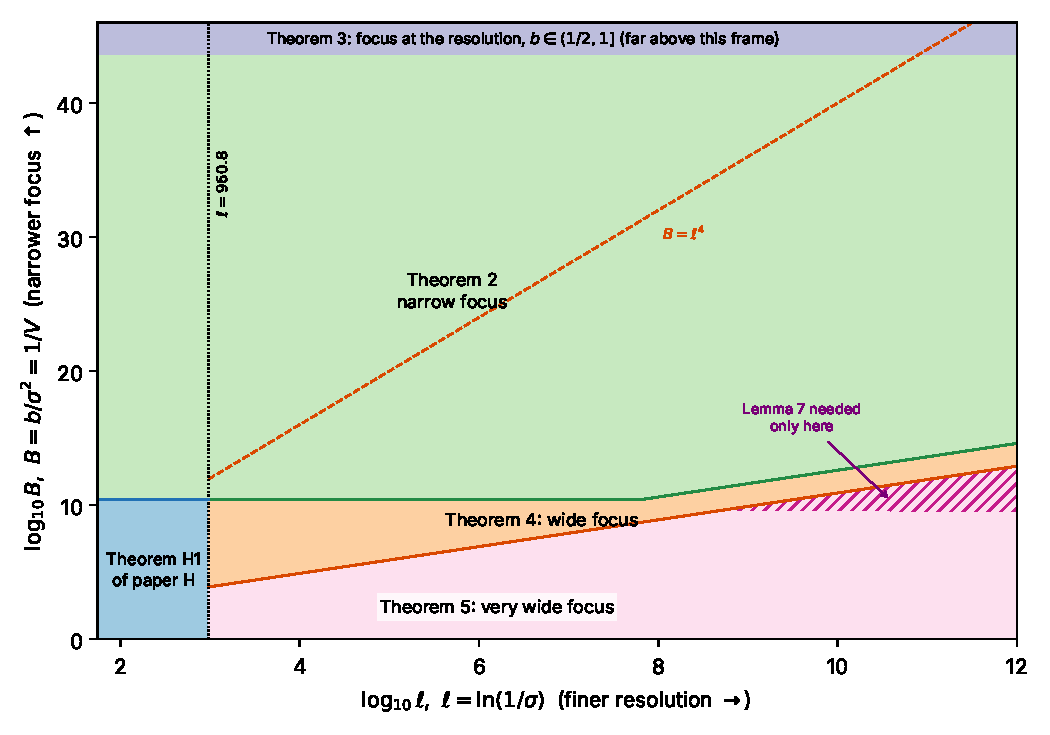
\includegraphics[width=\columnwidth]{figures/fig_map.pdf}
\caption{Which theorem covers which state. Horizontal axis: resolution, $\ell=\ln(1/\sigma)$. Vertical axis: narrowness of the focus, $B=b/\sigma^2$. The band at the top stands for $b\in(1/2,1]$, i.e.\ $B>e^{2\ell}/2$, which lies far above the frame. The region of Theorem~\ref{thm:verywide} continues below the frame down to $B\to0$. Hatched: the only states where Lemma~\ref{lem:P} is needed. The boundaries are the formulas of Table~\ref{tab:map}.}
\label{fig:map}
\end{figure}

\begin{table*}
\caption{The five theorems that cover the map, for windows with $\eta\le1/\ell$ in the regime $5\times10^{11}\sigma^2\le x\le0.003$. ``New'' means proved in this paper. The status labels are those of Papers~F and~H: \emph{proof} is closed by formulas alone; \emph{computer-assisted} uses finitely many interval-arithmetic computations as part of the proof.}
\label{tab:map}
\begin{ruledtabular}
\small
\begin{tabular}{p{0.12\textwidth}p{0.08\textwidth}p{0.26\textwidth}p{0.16\textwidth}p{0.15\textwidth}p{0.11\textwidth}}
focus & $\ell$ & $B=b/\sigma^2$ & theorem & bound on $g\sqrt\ell/(1-\bar\varepsilon)$ & status\\ \hline
at the resolution & $\ge55.26$ & $e^{2\ell}/2<B\le e^{2\ell}$ & Theorem~\ref{thm:res} (new) & $\ge0.19\sqrt\ell$ & proof\\
narrow & $\ge55.26$ & $\max(2.5\times10^{10},50(8\ell+100))\le B\le e^{2\ell}/2$ & Theorem~\ref{thm:narrow} (new) & $\ge\sqrt{1+10/\ell}$ & computer-assisted\\
wider than $0.7$ periods & $[55.26,960.8]$ & $B<2.5\times10^{10}$ & Theorem~H1 of~\cite{H} & $\ge1$ & computer-assisted\\
wide & $\ge960.8$ & $8\ell+100\le B<\ell^4$ & Theorem~\ref{thm:wide} (new) & $\ge\sqrt{1+10/\ell}$ & computer-assisted\\
very wide & $\ge960.8$ & $0<B\le8\ell+100$ & Theorem~\ref{thm:verywide} (new) & $\ge\sqrt{1+10/\ell}$ & proof\\
\end{tabular}
\end{ruledtabular}
\end{table*}

\emph{The two facts behind the very wide focus.}
When the focus spans many periods the observer no longer sees single ripples; what reaches her is the brightness averaged over a period.
The information she gets is the information in the slope of the ripple, multiplied by the phase mismatch between the centre and the edge of the focus, and the mismatch is as large as the focus is wide.
\begin{itemize}
\item \emph{Mean square instead of sup} (Proposition~\ref{prop:BE}).
  The enemy is a cross term between the curvature of the ripple and the phase mismatch.
  Paper~H measured it in mean square over the ripple rather than at its worst point, and used this only at the edge $B\le10^4$.
  We show that the heart of that argument depends neither on $B$ nor on $\ell$: the cross term costs at most $8\%$ of the slope information, whatever the width of the focus.
  Only the bookkeeping of the exponentially small remainders had to be redone.
\item \emph{Positivity and periodicity} (Lemma~\ref{lem:P}).
  If the focus spans only a few periods, averaging is not available.
  But the window is periodic along the ripple.
  Suppose a steep slope sits exactly where the phase mismatch vanishes, so that nothing can be read from it.
  The same slope is present one period away, and two periods away, and there the mismatch does not vanish.
  Those neighbours lie in the tail of the focus and are dim, but brightness is never negative, so they cannot cancel anything; they only count for less.
  The law asks for an amount of information of the order of the resolution itself, and the dim neighbours provide far more than that.
\end{itemize}
The second fact uses nothing but the shape of the window and the sign of the integrand; it may be of use elsewhere.

\emph{What is proved and what is not.}
We keep the distinction of Papers~F and~H between proof, computer-assisted proof, derivation, numerical evidence and conjecture, and mark every statement.
Table~\ref{tab:map} shows the status of the five theorems at a glance: two are proofs in the strict sense, three are computer-assisted.
The computer-assisted part consists of finitely many interval-arithmetic evaluations of explicit constants and conditions, with outward rounding, and of the certificates of Paper~H; it is listed in App.~\ref{app:C} and Table~\ref{tab:ca}.
We tried to break every claim before proving it.
For each one we report the families searched, the planted adversaries, and deliberately wrong versions that the same search does break (Sec.~\ref{sec:break}).
Direct two-dimensional quadrature reaches only $\ell\le10$, far from the range of the theorems; such comparisons are evidence about the formulas, not about the theorems, and are labelled \numst.

The limits of the result carry the same weight as the result.
\begin{itemize}
\item \emph{The window class.} The main theorem is for $\eta\le1/\ell$. Windows with a stronger ripple are outside it, except in two places: the very wide focus (Theorem~\ref{thm:verywide} needs no bound on $\eta$, so it holds for every window of the class), and the states of Paper~H's partial results. We make no claim beyond these.
\item \emph{The constant $\bar\varepsilon$.} Every bound carries the factor $1-\bar\varepsilon$ of condition (P6) of~\cite{F}. It is a hypothesis on the window class, not something we prove.
\item \emph{The regime.} We work in $5\times10^{11}\sigma^2\le x\le0.003$. The case $x\ge0.003$ is Theorem~48 of~\cite{F} (for $\sigma\le10^{-24}$); smaller $x$ is not treated.
\item \emph{The lower side only.} The upper side of the law is that of Paper~F and is not extended here.
\item \emph{Borrowed results.} Theorem~H1, the lower bound $g\ge(1-\bar\varepsilon)((a)+(a'))$, the brightness lemma CM-1, Lemma~R$_\theta$ and the mean-square step are taken from Papers~F and~H; the local lemmas behind the lines are new (App.~\ref{app:A}). Section~\ref{sec:main} says exactly which statement is borrowed and which is new.
\end{itemize}

\emph{Picture.}
A lens cannot be fooled by where it is pointed.
Narrow the focus to the resolution, and the background alone carries the information.
Widen it over hundreds of ripples, and the turning of the phase across the focus carries it.
In between, a short piece of ripple and the chirp share the load.
In every case what survives the blur is at least the fraction $1/\sqrt\ell$.

\section{Main theorem}
\label{sec:main}

\subsection{Setting}
We use the notation of Papers~F and~H and recall only what the statements need.
A periodic window is $p=\mathcal N_V\,\Gamma\,h/Z$, with $\mathcal N_V$ a Gaussian of variance $V=\sigma^2/b$ in $v$, $\Gamma=N(0,L^2)$ in $w$, and
\begin{gather}
h-1=e^{-w^2/2s^2}R(t),\quad t=k'v,\\ R(t)=\sum_{n\ge1}q0_n\cos(nt-\varphi_n).
\end{gather}
We write $x=(k'\sigma)^2$, $\tau=x/b$, $\eta=\sup|R|$ and $\ell=\ln(1/\sigma)$.
A \emph{state} is a choice of $(b,L^2,s^2)$ with $0<b\le1$, (P0) $L^2\le1/\sigma$ and (P4) $\sigma^2\le s^2\le L^2/4$.
The conditions (P0)--(P7) are those of Table~5 of~\cite{F}.
Throughout,
\begin{equation}
B=\frac{b}{\sigma^2}=\frac1V,\qquad \Gamma_\ell=\sqrt{\frac{1+10/\ell}{\ell}} .
\end{equation}
As in Eq.~(3) of~\cite{F},
\begin{equation}
g\ \ge\ (1-|\varepsilon|)\,\bigl((a)+(a')\bigr),\quad (a)=\frac{2A_w}{\sigma\,\mathrm{den}},\quad (a')=\frac{N_\phi}{\sigma\,\mathrm{den}},
\label{eq:ga}
\end{equation}
with $\mathrm{den}=\sigma^2(\Jvv+\Jww)$ and $|\varepsilon|\le\bar\varepsilon$ the window-class constant of (P6).
All theorems below bound $(a)+(a')$ from below; the factor $1-\bar\varepsilon$ enters only through Eq.~\eqref{eq:ga}.

\emph{The class.} A window is \emph{admissible} if it satisfies (P0), (P2)--(P4) and (P6), and $5\times10^{11}\sigma^2\le x\le0.003$.
This is the class of Theorem~H1 of~\cite{H}.

\subsection{Statement}

\begin{theorem}[every focus, every resolution] \status{proof, computer-assisted: Theorems~\ref{thm:narrow}, \ref{thm:wide} and Theorem~H1 of~\cite{H}}
\label{thm:main}
Let $\ell\ge55.26$ and let an admissible window satisfy $\eta\le1/\ell$.
Then every state satisfies
\begin{equation}
g\sqrt\ell\ \ge\ 1-\bar\varepsilon .
\end{equation}
If $\ell\ge960.8$, every state satisfies the stronger bound
\begin{equation}
g\sqrt\ell\ \ge\ (1-\bar\varepsilon)\sqrt{1+10/\ell}\,;
\end{equation}
for $55.26\le\ell<960.8$ the stronger bound holds for every state with $B\ge2.5\times10^{10}$.
\end{theorem}

In the observer's words: at every resolution finer than about $10^{-24}$, and for every position and width of the focus, the information that survives the blur is at least the fraction $(1-\bar\varepsilon)/\sqrt\ell$.
There is no state in which a clever focus does better than the exchange rate.

Theorem~\ref{thm:main} is assembled from five statements, each for one kind of focus.
Four are new; the fifth is Theorem~H1 of~\cite{H}.
We state them in the language of windows; the sections that prove them give the sharper technical forms.

\begin{theorem}[narrow focus] \status{proof, computer-assisted: Sec.~\ref{sec:narrow} and App.~\ref{app:C}}
\label{thm:narrow}
Let $\ell\ge55.26$ and let an admissible window satisfy $\eta\le1/\ell$.
Every state with
\begin{equation}
b\le\tfrac12,\qquad B\ge\max\bigl(2.5\times10^{10},\,50(8\ell+100)\bigr)
\end{equation}
satisfies $(a)+(a')\ge\Gamma_\ell$.
There is no upper limit on $\ell$.
\end{theorem}

\begin{theorem}[focus at the resolution] \proofst
\label{thm:res}
Let $\ell\ge55.26$ and let an admissible window satisfy $\eta\le1/\ell$.
Every state with $\tfrac12<b\le1$ satisfies $(a)+(a')\ge0.1995$; if the ripple has energy in the focus ($G>0$ in the notation of Sec.~\ref{sec:setting}) then $(a)+(a')\ge0.6$.
In particular $(a)+(a')\ge\Gamma_\ell$.
\end{theorem}

\begin{theorem}[wide focus] \status{proof, computer-assisted: Sec.~\ref{sec:wide} and App.~\ref{app:C}}
\label{thm:wide}
Let $\ell\ge960.8$ and let an admissible window satisfy $\eta\le1/\ell$.
Every state with $8\ell+100\le B<\ell^4$ satisfies $(a)+(a')\ge\Gamma_\ell$.
\end{theorem}

\begin{theorem}[very wide focus] \proofst
\label{thm:verywide}
Let $\ell\ge960.8$ and let a periodic window satisfy (P0), (P3), (P4) and $5\times10^{11}\sigma^2\le x\le0.003$.
Every state with $0<B\le8\ell+100$ satisfies $(a)+(a')\ge\Gamma_\ell$.
Neither $\eta\le1/\ell$ nor (P2) is used.
\end{theorem}

Theorem~\ref{thm:verywide} follows from the next two statements; the first holds where the focus spans many periods, the second everywhere.
Put $\tau_0(\ell)=4\ln\ell+40$.

\begin{proposition}[the mean-square bound without limits on $B$ and $\ell$] \proofst
\label{prop:BE}
Under the hypotheses of Theorem~\ref{thm:verywide}, every state with $0<B\le8\ell+100$ and $\tau\ge\tau_0(\ell)$ satisfies
\begin{equation}
(a)+(a')\ \ge\ \frac{\kappa(B)}{\sigma},\qquad \kappa(B)=\min\Bigl(0.055,\ \frac{0.459}{4B+1}\Bigr).
\end{equation}
\end{proposition}

\begin{lemma}[positivity and periodicity] \proofst
\label{lem:P}
Let $p=\mathcal N_V\,\Gamma\,h/Z$ with $h$ as above, $\sum_nq0_n\le\Qb=\tfrac14$, $s\ge\sigma$ and $2\pi\sigma/\sqrt x\le1$; the density $\Gamma$ of $w$ may be any positive differentiable density.
Let $N_1=\sum_nn\,q0_n$,
\begin{equation}
a=\frac{\sqrt x\,N_1}{1-\Qb}+\frac{\Qb e^{-1/2}}{1-\Qb},\qquad \theta=\tfrac15e^{-10\pi^2/\tau}.
\end{equation}
Then every state satisfies
\begin{equation}
N_\phi\ \ge\ c_P\,\sigma^2\Jvv,\qquad c_P=\frac{\sigma^2}{8x}\,\frac{\theta}{1+\theta}\Bigl((1-b)-\frac{2a\sqrt x}{\pi}\Bigr)_+^2 .
\end{equation}
\end{lemma}

Proposition~\ref{prop:BE} is Lemma~BE of~\cite{H} with its two restrictions ($B\le10^4$, $\ell\le6907.8$) removed; for $B\le10^4$ its constant $0.459/(4B+1)\ge1.147\times10^{-5}$ agrees with the constant $1.1\times10^{-5}$ of~\cite{H}.
Lemma~\ref{lem:P} is new.
It does not use (P0), the regime of $x$, or any bound on $\eta$.

\subsection{Proof of Theorem~\ref{thm:main} from the five statements}

\begin{proof}
By Eq.~\eqref{eq:ga} it suffices to bound $(a)+(a')$.
Fix a state and write $B=b/\sigma^2$.

\emph{Case $55.26\le\ell\le960.8$.}
If $b>\tfrac12$, Theorem~\ref{thm:res} applies.
Let $b\le\tfrac12$.
On this range of $\ell$, $50(8\ell+100)\le389\,320<2.5\times10^{10}$.
If $B\ge2.5\times10^{10}$, Theorem~\ref{thm:narrow} gives $(a)+(a')\ge\Gamma_\ell$.
If $B<2.5\times10^{10}$, then $\tau=x/b\ge5\times10^{11}/B>20$, and item~(i) of Theorem~H1 of~\cite{H} gives $g\sqrt\ell\ge1-\bar\varepsilon$.

\emph{Case $\ell\ge960.8$.}
If $b>\tfrac12$, Theorem~\ref{thm:res} applies.
If $B\le8\ell+100$, Theorem~\ref{thm:verywide} applies.
If $8\ell+100\le B<\ell^4$, Theorem~\ref{thm:wide} applies.
If $B\ge\ell^4$ and $b\le\tfrac12$, then $B\ge\max(2.5\times10^{10},50(8\ell+100))$, because $\ell^4\ge8.5\times10^{11}$ and $\ell^4\ge50(8\ell+100)$ for $\ell\ge960.8$, and Theorem~\ref{thm:narrow} applies.
These cases exhaust the states, and each gives $(a)+(a')\ge\Gamma_\ell$, i.e.\ $g\sqrt\ell\ge(1-\bar\varepsilon)\sqrt{1+10/\ell}$.
\end{proof}

\subsection{Proof of Theorem~\ref{thm:verywide} from Proposition~\ref{prop:BE} and Lemma~\ref{lem:P}}

\begin{proof}
Let $\tau\ge\tau_0(\ell)$.
Proposition~\ref{prop:BE} and $B\le8\ell+100$ give $(a)+(a')\ge0.459\,e^{\ell}/(32\ell+401)$, which exceeds $\Gamma_\ell$ by a factor larger than $e^{950}$ for $\ell\ge960.8$.

Let $\tau<\tau_0(\ell)$.
Since $2A_w\ge\sigma^2\Jww$ (because $0\le\phi\le2$) and $\mathrm{den}=\sigma^2\Jvv+\sigma^2\Jww$, Lemma~\ref{lem:P} gives
\begin{equation}
2A_w+N_\phi\ \ge\ \sigma^2\Jww+c_P\,\sigma^2\Jvv\ \ge\ \min(1,c_P)\,\mathrm{den},
\end{equation}
so it suffices to show $c_P\ge\sigma\Gamma_\ell$.
The regime gives $\tau B=x/\sigma^2\ge5\times10^{11}$, hence $\tau\ge5\times10^{11}/(8\ell+100)$ and $10\pi^2/\tau\le10\pi^2(8\ell+100)/(5\times10^{11})$; also $x=\tau B\sigma^2<\tau_0(\ell)(8\ell+100)\sigma^2$, and the condition $2\pi\sigma/\sqrt x\le1$ of the lemma holds.
With $\theta/(1+\theta)\ge\tfrac16e^{-10\pi^2/\tau}$ and the bracket of $c_P$ above $1-10^{-400}$,
\begin{equation}
\begin{split}
\ln\frac{c_P}{\sigma\Gamma_\ell}\ \ge\ &\ell-\frac{10\pi^2(8\ell+100)}{5\times10^{11}}\\&-\ln\bigl(48\,\tau_0(\ell)(8\ell+100)\bigr)-\ln\Gamma_\ell-10^{-399}.
\end{split}
\end{equation}
The right side is at least $947$ at $\ell=960.8$ and increases with $\ell$.
\end{proof}

States with $\tau<\tau_0(\ell)$ exist in the region of Theorem~\ref{thm:verywide} only for $\ell>5.19\times10^{8}$ and $B>5\times10^{11}/\tau_0(\ell)$ (the hatched strip of Fig.~\ref{fig:map}); below that resolution Proposition~\ref{prop:BE} alone proves the theorem.

\subsection{What is new and what is borrowed}

\begin{table}
\caption{Origin of the statements used in Theorem~\ref{thm:main}.}
\label{tab:origin}
\begin{ruledtabular}
\small
\begin{tabular}{p{0.56\columnwidth}p{0.36\columnwidth}}
statement & origin\\ \hline
$g\ge(1-\bar\varepsilon)((a)+(a'))$, the conditions (P0), (P2)--(P4), (P6) & Paper~F, Eq.~(3), Table~5\\
period-average lemmas (Lemmas~19, 21--23 of F) & Paper~F, App.~D\\
Theorem~H1 ($\tau\ge20$, $\ell\le960.8$) & Paper~H, \Hsec{VIII}\\
Lemma~R$_\theta$ (local route), Lemma~CM-1, second line of Lemma~CN-1 & Paper~H, \Hsec{IX~A}\\
Lemma~A4*, the steps of Lemma~BE, window constants $U_1,U_2,\gamma_P,c_\chi$ & Paper~H, \Hsecs{III, VI, VII and Apps.~D, E}\\
the local lemmas (direct form, main-term identity, ring, pair; Lemmas~\ref{lem:lines}--\ref{lem:G0} and App.~\ref{app:A}) & new\\
Theorems~\ref{thm:narrow}, \ref{thm:res}, \ref{thm:wide}, \ref{thm:verywide} & new\\
Proposition~\ref{prop:BE} (Lemma~BE for all $B\le8\ell+100$, all $\ell\ge960.8$) & new; same core as Lemma~BE\\
Lemma~\ref{lem:P} (positivity and periodicity) & new\\
the brightness hypothesis (H$'$) in closed form, the lines and their constants & new (Secs.~\ref{sec:setting}--\ref{sec:wide})\\
\end{tabular}
\end{ruledtabular}
\end{table}

Table~\ref{tab:origin} separates the two.
Three remarks on the hypotheses.
First, $\eta\le1/\ell$ enters Theorems~\ref{thm:narrow}, \ref{thm:res} and~\ref{thm:wide} through the sandwich factors $1/(1\pm\eta)$ written into the lines, and Theorem~H1 through its item~(i); Theorem~\ref{thm:verywide} does not need it.
Second, the bound $q0_n\le2e^{-n^2x/2}$ used in Proposition~\ref{prop:BE} holds for every window of~\cite{F}, as noted in~\cite{H}.
Third, the factor $1-\bar\varepsilon$ is the hypothesis (P6); every statement of this paper is a statement about $(a)+(a')$ and is independent of the value of $\bar\varepsilon$.


\section{Setting and the local route}
\label{sec:setting}

This section collects what Theorems~\ref{thm:narrow}--\ref{thm:wide} share: the quantities of the focus, the \emph{lines} (explicit lower bounds for the numerator of $(a)+(a')$), and the hypothesis on the brightness of the ripple inside the focus.
Theorem~\ref{thm:verywide} uses none of it; Section~\ref{sec:verywide} can be read on its own.

\subsection{The quantities of the focus}

Fix a state and a focus $t_0$ on the ripple.
Averages $\langle\cdot\rangle$ are taken with the Gaussian $\theta_\tau$ of variance $\tau=x/b$ centred at $t_0$, as in \Hsec{IX~A} of~\cite{H}.
With $u=t-t_0$ we write
\begin{gather}
E_0=\langle\theta_\tau R^2\rangle,\quad E_1=\langle\theta_\tau R'^2\rangle,\quad \mu=\frac{xE_1}{E_0},\nonumber\\ P=2xE_1,\qquad \kappa=\frac{\langle(u^2/\tau)\theta_\tau R'^2\rangle}{E_1}.
\label{eq:focusq}
\end{gather}
$\mu$ measures how fine the ripple is in the focus, $P$ how bright it is, and $\kappa$ how far from the centre of the focus its brightness sits ($\kappa=1$ when the brightness is spread evenly over a focus that spans many periods).
The envelope enters through
\begin{gather}
r=\frac{s^2}{L^2}\in[\sigma^3,\tfrac14],\qquad a=\frac{4\sigma}{L^2}\in\Bigl[4\sigma^2,\frac{4r}{\sigma}\Bigr],\nonumber\\ g_s=\sqrt{\frac{r}{2+r}},\qquad G=g_sP,\qquad k_E=\sqrt{\frac{r}{1+r}} .
\end{gather}
The two ends of $a$ are (P0) $L^2\le1/\sigma$ and (P4) $s\ge\sigma$; $G$ is the brightness of the ripple as the observer's lens sees it.
The target of Theorems~\ref{thm:narrow}--\ref{thm:wide} is
\begin{gather}
\mathrm{Num}-\gamma\,\sigma\,\mathrm{den}\ \ge\ 0,\nonumber\\ \mathrm{Num}=2A_w+N_\phi,\qquad \gamma=\Gamma_\ell=\sqrt{(1+10/\ell)/\ell},
\label{eq:target}
\end{gather}
which is $(a)+(a')\ge\Gamma_\ell$.
Throughout Secs.~\ref{sec:setting}--\ref{sec:wide}, $\eta=1/\ell$ is used in the coefficients (the window class has $\eta\le1/\ell$), $U_1=\tfrac14\sqrt{2\ell+3.1}+10^{-6}$ is the window constant of~\cite{H} (\Hsec{VI}; valid for $x\ge5\times10^{11}\sigma^2$, with no upper limit on $\ell$), and $X_1=\tfrac43U_1$.

\subsection{The lines}
\label{sec:lines}

\begin{lemma}[the lines are lower bounds] \status{proof for $y\le10^{-40}$ (used in Theorem~\ref{thm:res}); for $y\le10^{-4}$ three constants are computer-assisted (App.~\ref{app:A})}
\label{lem:lines}
Let $\ell\ge55.26$, $b\le\tfrac12$, $B\ge8\ell+100$ and $y=(1-b)^2/(2B)\le10^{-4}$, and let the window satisfy $\eta\le1/\ell$, (P3) and $\sqrt x\,\sup|R'|\le U_1$.
For each of the options $k\in\{\mathrm{Fz},\ \mathrm{Tz\text{-}B2},\ \mathrm{Tz\text{-}B1}\}$ and every $a$ in its range,
\begin{equation}
\frac{\mathrm{Num}-\gamma\sigma\,\mathrm{den}}{\sigma}\ \ge\ \Lambda_k(a):=\sum_{l\in k}s_l\,c_l\,\sigma^{p_l-1}f_{t_l}(a),
\label{eq:lines}
\end{equation}
where the sum runs over the lines of the option, $s_l=\pm1$, $c_l>0$ is a coefficient free of $\sigma$ (written with $B=b/\sigma^2$), $p_l$ is a power, and the type $t_l$ fixes the $a$-dependence: $f_L=a$, $f_S=\sqrt a$, $f_C=1$, $f_M=1/\sqrt a$, $f_H=1/(a+\sigma)$.
For $b\in(\tfrac12,1]$ the same holds for the option Fz.
\end{lemma}

The $37$ lines and their coefficients are listed in App.~\ref{app:B}.
Each line is a term of one of the local lemmas, written in the same form or in a worse one (a gain made smaller, a loss made larger).
The local lemmas are a direct form of the $v$-branch (an identity), an identity for its main term, a bound for a ring of the Gaussian tail, and a lemma for the pair (III)$+$B1v that carries the chirp; together with Lemma~R$_\theta$ of~\cite{H} (\Hsec{IX~A}) for the $w$-branch they give the lines.
They are new and are proved in App.~\ref{app:A}.
None of them has a restriction on $\ell$, $\mu$ or $\kappa$; $\ell$ enters only through $U_1$, $\eta=1/\ell$ and the ring radius $K^2=8\ell+100$.
The condition on $B$ is $z_0^2=K^2y\le1$ with $y=(1-b)^2/(2B)$ for the pair lemma, $1-q>0$ for the ring, and $y\le10^{-4}$ for three constants of the main-term identity (Lemmas~\ref{lem:M4} and~\ref{lem:M12}, computer-assisted); for $y\le10^{-40}$, which covers Theorem~\ref{thm:res}, these constants are bounded by hand (Lemma~\ref{lem:M0}).
For the option Fz with $b>\tfrac12$, the pair lemma is not used; Fz is a weaker lower bound from which a positive line is subtracted (App.~\ref{app:A}).

\begin{table}
\caption{The lines that carry the proofs. ``$\times\sigma$'' is the unit of Eq.~\eqref{eq:lines}. The other lines (remainders of size $\sigma^{1/2}$ or smaller relative to these, and the losses of the branches B1, B2) are listed in App.~\ref{app:B}.}
\label{tab:lines}
\begin{ruledtabular}
\small
\begin{tabular}{p{0.11\columnwidth}p{0.07\columnwidth}p{0.47\columnwidth}p{0.2\columnwidth}}
line & type & value & meaning\\ \hline
P1 & L & $+a/2$ & $w$-information\\
P4z & H & $+(b\omega/2)/(a+\sigma)$ & background in $v$\\
P2z & L & $+\alpha Ga$ & ripple, $w$-side\\
hFz & H & $+\beta G/(a+\sigma)$ & ripple, $v$-side\\
cKz & C & $+\chi G$, $\chi=\mathrm{fl}\,k_f\kappa\sigma/(16b)$ & chirp\\
d1, d2 & C & $-\gamma bk_1$, $-\gamma Gk_2$ & target (den)\\
N1, N2 & L & $-\varepsilon_1(r)\,a/2$, $-Q_2\,a/(16B)$ & $w$-branch\\
hneg1 & H & $-\varepsilon_h(r)\,(b\omega/2)/(a+\sigma)$ & main term\\
FzK & C & $-\sigma\kappa G/(4(1-\eta))$ & option Fz\\
\end{tabular}
\end{ruledtabular}
\end{table}

Table~\ref{tab:lines} shows the lines that carry the proofs.
Here $\omega=(1+3/(4B))^{-2}$, $\mathrm{fl}=1/(1+\eta)$, $k_f=(1-b)^2\,\mathrm{brk}$, $\mathrm{brk}=1-4b/(1-b)-z_2/12$, $z_2=(8\ell+100)/(2B)$, $q=(8\ell+100)(1+\eta)/(8B(1-\eta))$, $k_1=1+(\eta+0.184)k_E$, $k_2=1/(2(1-\eta))$, $\varepsilon_1(r)=\eta k_E(2+r)/(1+r)$, $\varepsilon_h(r)=2k_E(\eta+0.184)/\omega$, and $\alpha$, $\beta$, $Q_2$ are explicit (App.~\ref{app:B}).
Every coefficient is a product of positive factors in the class, so the sign of each line is that of the table for every $\ell$ \proofst.
The options differ in how they pay for the pair (III)$+$B1v: Fz drops the chirp and pays the line FzK; Tz uses the chirp cKz and pays the branch losses B2 (Tz-B2) or B1 (Tz-B1).
Since every option is a lower bound of the same quantity, the option may be chosen state by state and $a$ by $a$.

\subsection{The brightness hypothesis}

\begin{lemma}[the brightness hypothesis (H$'$)] \proofst
\label{lem:Hprime}
For every window of the class and every focus, $P$ satisfies
\begin{itemize}
\item[(A)] $P\le\mu/8$;
\item[(K)] $\kappa P\le2U_1^2$;
\item[(CM)] $P/2\le\mathcal U(P;\mu,b,1,1)$;
\item[(J)] for all $\lambda>0$ and $\kappa_b\ge\kappa$ with $b\le\lambda\kappa_b\le1$: $P/2\le\mathcal U(P;\mu,b,\sqrt{\lambda\kappa_b},e^{1/(2\lambda)})$,
\end{itemize}
where, with $b'=b/s^2$, $\hat E=\min(P/(2\mu s),1/16)$ and $B_0(E,b')=(1+\sqrt E+(E/2)^{1/(2+b')})^2$,
\begin{gather}
\mathcal U(P;\mu,b,s,c)=c\Bigl[(1+\tfrac{b'}2)\,s\,\hat E\ln\frac{2B_0(\hat E,b')}{\hat E}+c_{\rm CM}\,b'\,s\Bigr],\nonumber\\ c_{\rm CM}=\frac{\sqrt2}{16e}.
\end{gather}
\end{lemma}

\begin{proof}[Origin of the four parts]
(A) is $E_0\le\Qb^2=1/16$, from (P3).
(K) is $x E_1\kappa\le x\sup R'^2\le U_1^2$.
(CM) is Lemma~CM-1 of~\cite{H} (\Hsec{IX~A}) with $E_0'\le1/16$; the constant $c_{\rm CM}$ is the factor $(\sqrt2/e)E_0'$ of that lemma.
(J) uses Lemma~CM-1 at a second focus $\tau'=\lambda\kappa_b\tau$, the second line of Lemma~CN-1 of~\cite{H} (\Hsec{IX~A}), and the inequality
$E_1^{(\tau)}\le\sqrt{\tau'/\tau}\,\exp\bigl(\kappa(\tau/\tau'-1)/2\bigr)E_1^{(\tau')}$ for all $\tau'>0$, which is Jensen's inequality for the convex function $z\mapsto e^{-cz}$ of $z=u^2$ (App.~\ref{app:A}).
We use (J) only with $b'=b/(\lambda\kappa_b)\le\tfrac1{16}$.
\end{proof}

No condition on $\mu$ is needed; Lemma~CM-1 and the two-foci inequality hold for every $\mu>0$.
The four parts are consequences of positivity of the window and of the class bounds; they are not assumptions on the window, but we keep the name (H$'$) of the earlier work.
Two closed forms are used in the proofs.

\begin{lemma}[closed forms] \proofst
\label{lem:DI}
Let $A=1+b/2$, $\bar B=B_0(\tfrac1{16},b)$ and suppose $\mu>A\ln(32\bar B)+16c_{\rm CM}b$.
\begin{itemize}
\item[(v)] For every $t>0$: $P/(2\mu)\le\max\bigl(2\bar Be^{-\mu/A+t},\ c_{\rm CM}b/((1+b/2)t)\bigr)$.
\item[(iv)] $P\le4\mu B_1e^{-\mu/(1+b/2)}+2c_{\rm CM}\mu b/(1+b/2)$, with $B_1=B_0(y_1,b)$, $y_1=2\bar Be^{-\mu/A}+c_{\rm CM}b$.
\item[(K)] If $\mu\ge6$, $\kappa\le\kappa_b\le1/\mu$ and $\kappa_b\ge16be^{\mu}/\mu$, then
\begin{gather}
P\le4\mu e^{-\mu}\sqrt{e\mu\kappa_b}\,E_J(\mu),\quad\text{where}\nonumber\\ E_J(\mu)=(1+4.43e^{-\mu/2})^2e^{\mu e^{-\mu}/32}+6.2\times10^{-4}.
\end{gather}
\end{itemize}
\end{lemma}

The proofs are short consequences of (CM) and (J) (App.~\ref{app:A}).
The constant $E_J$ is proved by hand: every quantity in it is monotone in $\mu$, which reduces the claim to the single point $\mu=6$, where seven numbers are checked; the same numbers were also confirmed by interval arithmetic.

\subsection{States without a visible ripple}

\begin{lemma}[$G=0$] \proofst
\label{lem:G0}
If $P=0$, then for every $\sigma>0$, $b\in(0,1]$ and $L^2\ge4\sigma^2$, and for every $\tau$, $\mu$, $\kappa$, $x$,
\begin{gather}
(a)+(a')\ \ge\ \min\Bigl(\frac{0.316}{\sigma},\ \frac{C_0}{\sqrt b}\Bigr),\nonumber\\ C_0=\tfrac32\sqrt{k/128}=0.19950\ldots,\qquad k=3-2/e.
\end{gather}
\end{lemma}

The proof (App.~\ref{app:A}) computes $(a)+(a')$ in closed form: with no ripple the window is Gaussian, $m_z$ is linear in the two Gaussian coordinates, and $\E[X^2\cos(aX+cY)]=(1-a^2)e^{-(a^2+c^2)/2}$.
Since $C_0=0.1995>\Gamma_\ell$ for $\ell\ge55.26$ ($\Gamma_{55.26}=0.14619$), states with $G=0$ satisfy the law in every region.

\emph{Picture.}
The focus is a Gaussian spot on the ripple.
Three numbers describe what the observer sees inside it: how fine the ripple is ($\mu$), how bright it is ($P$), and whether the brightness sits at the centre of the spot or is spread over it ($\kappa$).
Positivity of the window forbids a ripple that is fine, bright and concentrated at once; this is Lemma~\ref{lem:Hprime}.
The lines are the bookkeeping: each says how much information one part of the picture carries, or how much one effect of the blur takes away.

\section{Narrow focus (Theorem~\ref{thm:narrow})}
\label{sec:narrow}

\subsection{Technical form and the rule}

\begin{proposition}[narrow focus, line form] \caproofst{Sec.~\ref{sec:ca} and App.~\ref{app:C}}
\label{prop:narrow}
Let $\ell\ge55.26$.
Let a state satisfy $\mu>0$, $\sigma^3\le r\le\tfrac14$, $B\ge\max(2.5\times10^{10},\,50(8\ell+100))$, $b\le\tfrac12$, $\kappa>0$, and let $P>0$ satisfy (H$'$) (Lemma~\ref{lem:Hprime}).
Then for every $a\in(0,4r/\sigma]$ the option $k$ chosen by the rule below satisfies $\Lambda_k(a)\ge0$ with $\gamma=\Gamma_\ell$.
There is no upper limit on $\ell$.
\end{proposition}

\emph{The rule.}
Put $c_1=0.78$, $c_T=3.5$, $c_{\rm ch}=2.9$, $\Gamma_2=\Gamma_\ell k_2$, $a_s=4c_m^2\ell^6\sigma^3/r$ with $c_m=2X_1\sqrt{2+r}/((1-\eta)\,\mathrm{fl}\,(1-z_2/2)\sqrt{2\pi})$.
\begin{itemize}
\item \emph{Case I} ($G\le c_1\sqrt b/\Gamma_2$): if $b<0.1$ and $\kappa\ge c_T\sqrt\ell\,b/\sigma$, use Tz-B2; otherwise Fz.
\item \emph{Case II} ($G>c_1\sqrt b/\Gamma_2$): if $r\le c_{\rm ch}\sqrt\ell\,\sigma$, use Tz-B2 for every $a$; otherwise Tz-B2 for $a<a_s$ and Tz-B1 for $a\ge a_s$.
\end{itemize}
In Case~I the ripple is dark against the background, and the two background lines P1 and P4z pay for the target.
In Case~II the ripple is brighter than the background; the ripple lines P2z, hFz and the chirp cKz are needed.

\begin{proof}[Proof of Theorem~\ref{thm:narrow} from Proposition~\ref{prop:narrow}]
If $G>0$, Lemma~\ref{lem:lines} and Proposition~\ref{prop:narrow} give $(\mathrm{Num}-\Gamma_\ell\sigma\,\mathrm{den})/\sigma\ge\Lambda_k(a)\ge0$ at the state's own $a=4\sigma/L^2$.
If $G=0$, Lemma~\ref{lem:G0} gives $(a)+(a')\ge0.1995>\Gamma_\ell$.
\end{proof}

All numbers below are values at $\ell=55.26$, which is the hardest point for almost all of them.
That every quoted number and every condition holds for \emph{all} $\ell\ge55.26$ is the computer-assisted part (Sec.~\ref{sec:ca}).
Quantities that contain $B$ are bounded uniformly with $B\ge2.5\times10^{10}$, $q\le(1+\eta)/(400(1-\eta))$ and $z_2\le0.01$.

\subsection{Ceilings from the brightness hypothesis}

\begin{itemize}
\item[(F1)] $P\le0.7008$. In (CM), $\hat E\le1/16$, $E\ln(2B_0/E)$ increases on $(0,1/16]$, $B_0$ increases in $b$, and $B_0(1/16,1/2)=2.25$; hence $P\le2[(1.25/16)\ln72+c_{\rm CM}/2]$.
\item[(F2)] If $\max(\kappa,16b)\le\kappa_b\le1$, then $P\le w_{16}\sqrt{\kappa_b}$ with $w_{16}=e^{1/2}[(1+1/32)(1/8)\ln(32B_0(1/16,1/16))+2c_{\rm CM}/16]\le0.8972$ ((J) with $\lambda=1$).
\item[(F3), (F4)] Lemma~\ref{lem:DI}, items (iv)--(v) and (K).
\end{itemize}

\subsection{Remainders}
\label{sec:R}

With $\mathrm{es}=10^{-11}$ and $\mathrm{es}_\sigma=\ell^2e^{-\ell}$:
\begin{itemize}
\item[(R1)] N1 $=\varepsilon_1(r)\,$P1 with $\varepsilon_1\le0.01457$; the other L-lines satisfy $\mathrm{N2}+\mathrm{d3}+\mathrm{N4}+\mathrm{ring2}+\mathrm{A2a}+\mathrm{A2b}+\mathrm{B2b}\le0.52\,\mathrm{es}\,$P1, the largest part being $\mathrm{N2}/\mathrm{P1}=Q_2/(8B)\le0.507284\,\mathrm{es}$; d4$+$N4G and B1l are at most $\mathrm{es}_\sigma\,$P2z.
\item[(R2)] hneg1 $=\varepsilon_h(r)\,$P4z with $\varepsilon_h\le0.1808$.
\item[(R3)] The S-lines are $c_Sb\sqrt{\sigma a}$ with $c_S\le0.155$, at most $0.48\,\mathrm{es}$ times P4z ($a\le1$) or P1 ($a\ge1$).
\item[(R4)] The constant lines satisfy $\mathrm{N3}+\mathrm{M0Xi}+\mathrm{A1v}+\mathrm{pair}\le1.77\sigma$. With $e_0=1.26\times10^{-5}$, $m_1=1-\varepsilon_1-e_0$, $m_4=1-\varepsilon_h-e_0$, for all $a\ge0$
\begin{equation}
\begin{split}
&(1-\varepsilon_1-\mathrm{es})\frac a2+(1-\varepsilon_h-\mathrm{es})\frac{b\omega/2}{a+\sigma}-1.77\sigma\\&\qquad\ge\ m_1\frac a2+m_4\frac{b\omega/2}{a+\sigma},
\end{split}
\end{equation}
because $\mathrm{P1}+\mathrm{P4z}\ge\sqrt{b\omega}-\sigma/2\ge1.58\times10^5\sigma$ when $B\ge2.5\times10^{10}$. This is where the lower end of $B$ is used.
Then $m_1a/2+m_4(b\omega/2)/(a+\sigma)\ge\sqrt{m_1m_4b\omega}-\sigma/2\ge\Gamma_\ell bk_1+c_{1F}\sqrt b$ with $c_{1F}\ge0.7857$.
\item[(R5)] In Case~I, if $b\ge0.1$ or $\kappa<c_T\sqrt\ell\,b/\sigma$, the loss of Fz is $K_F=\mathrm{FzK}+\mathrm{A2k}+\mathrm{B2a}\le1.01\times10^{-3}\sqrt b$ (from $G\le c_1\sqrt b/\Gamma_2$ for small $b$, and from (K) otherwise).
\item[(R6)] For $a\le4r/\sigma$ the branch B2 costs $\mathrm{B2c}+\mathrm{B2s}\le c_{B2}G$, $c_{B2}=X_1/(4\sqrt2(1-\eta))+c_s/(4(1-\eta))\le0.0896\sqrt\ell$. This is where the upper end of $a$ is used.
\item[(R7)] In Case~II with $r>c_{\rm ch}\sqrt\ell\sigma$ and $a\ge a_s$: $\mathrm{B1m}\le\ell^{-3}\,\mathrm{hFz}+\mathrm{es}_\sigma\mathrm{P2z}$, $\mathrm{B1c}\le\mathrm{es}_\sigma\Gamma_2G$, and $\mathrm{uB2c}+\mathrm{uB2s}+\mathrm{A2k}+\mathrm{B2a}\le(c_u\sqrt r+2.1b^2)\,\mathrm{cKz}$ with $c_u\le0.48$.
\end{itemize}
The es-budget is shared: P1 carries $0.52\,\mathrm{es}$ from (R1) and, for $a\ge1$, $0.48\,\mathrm{es}$ from (R3); P4z carries $0.48\,\mathrm{es}$ for $a\le1$.
The lower end $r\ge\sigma^3$ is used only in (R1), through the factors $1/\sqrt r$ of A2b, B2b and ring2.

\subsection{Case I}

\emph{Option Fz.} By (R1)--(R5),
\begin{equation}
\Lambda_{\rm Fz}\ \ge\ (c_{1F}-1.01\times10^{-3})\sqrt b-\Gamma_2G\ \ge\ 0,
\end{equation}
since $G\le c_1\sqrt b/\Gamma_2$ and $c_{1F}-1.01\times10^{-3}\ge c_1=0.78$.

\emph{Option Tz-B2} ($b<0.1$, $\kappa\ge c_T\sqrt\ell b/\sigma$). The background part is the same; it remains to show $\mathrm{cKz}-\mathrm{B2c}-\mathrm{B2s}-\mathrm{A2k}-\mathrm{B2a}\ge0$.
For $b<0.1$, $k_f\ge0.4493$ and $\mathrm{cKz}\ge c_K\kappa\sigma G/b$ with $c_K=\mathrm{fl}\,k_f/16\ge0.02758$; moreover $\mathrm{A2k}\le0.04616\,\mathrm{cKz}$ and $\mathrm{B2a}\le10^{-6}\,\mathrm{cKz}$.
What is needed is $(1-0.04616-10^{-6})c_Kc_T\sqrt\ell\ge c_{B2}$: at $\ell=55.26$ the two sides are $0.6845$ and $0.6656$.

\subsection{Case II forces a chirp}

In Case~II, $G^2>c_1^2b/\Gamma_2^2\ge1.9863\,\ell b$, while $G^2\le(r/2)P^2$.
\begin{itemize}
\item[(c1)] $G\le P/3$ gives $b<c_bP^2$ with $c_b=(\Gamma_2/(3c_1))^2\le0.05593/\ell$; with (F1), $b\le0.0275/\ell$, and (CM) used again gives $P\le P_{\rm II}=0.5223$. Then $\mathrm{brk}\ge0.998$, so the Tz options are available.
\item[(b.1)] For $\mu>5.61$, Lemma~\ref{lem:DI}(v) with $t=\mu/(2A)$ gives $P\le9\mu e^{-0.4\mu}$; two passes of Lemma~\ref{lem:DI}(iv) give, for $\mu\ge7.44$, $P\le4\mu e^{-\mu}E_{\rm CM}$, $E_{\rm CM}=(1+3.445e^{-\mu/2})^2(1+2\times10^{-3}/\ell)$.
\item[(b.2)] $\mu<\ell+\ln\ell$: otherwise $G\le1.5\sigma$, while Case~II has $G\ge2.2\times10^5\sqrt\ell\,\sigma$.
\item[(c2)] If $\kappa\le1$: $\kappa>c_\kappa\ell b/r$ with $c_\kappa=2c_1^2/(\Gamma_2^2\ell w_{16}^2)\ge4.935$ (from (F2) with $\kappa_b=\max(\kappa,16b)$, and $\kappa_b=16b$ is impossible). Hence $\chi>\mathrm{fl}\,k_fc_\kappa\ell\sigma/(16r)$.
\item[(c3)] If $\kappa>1$: $b<(\Gamma_2^2/c_1^2)(r/2)P_{\rm II}^2$, hence $\chi>\mathrm{fl}\,k_fc_1^2\sigma/(8\Gamma_2^2P_{\rm II}^2r)$.
\end{itemize}
In words: a ripple that is brighter than the background cannot keep its brightness at the centre of the focus, because a concentrated ripple is dark (F2).
So in Case~II, $\kappa$ is large compared with $b/r$, and the chirp gain $\chi G$ is always there.

\subsection{Case II, three regions}

\emph{(II-ch) $r\le c_{\rm ch}\sqrt\ell\sigma$, option Tz-B2.}
$\Lambda\ge(1-\mathrm{es}_\sigma)\mathrm{P2z}+\mathrm{hFz}+(1-10^{-3})\chi G-c_{B2}G-\Gamma_2G$, and (c2)--(c3) give $(1-10^{-3})\chi\ge0.1041\sqrt\ell$, while $c_{B2}+\Gamma_2\le0.0996\sqrt\ell$.

\emph{(II-s) $r>c_{\rm ch}\sqrt\ell\sigma$, $a<a_s$, option Tz-B2.}
Here $a_s\le\ell^7\sigma^2\le10^{-9}\sigma$, so $\mathrm{hFz}\ge0.1085(r/\sigma)G\ge0.3149\sqrt\ell\,G\ge(c_{B2}+\Gamma_2)G$.

\emph{(II-m) $r>c_{\rm ch}\sqrt\ell\sigma$, $a\ge a_s$, option Tz-B1.}
Collecting (R), for every $a\ge a_s$,
\begin{equation}
\Lambda_{\rm Tz\text{-}B1}(a)\ \ge\ Xa+\frac{Y}{a+\sigma}+m_5\chi G-\Gamma_2G\,(m_T+T),
\label{eq:IIm}
\end{equation}
with $X=m_1/2+m_2\alpha G$, $Y=m_4b\omega/2+m_3\beta G$, $m_2=1-3\mathrm{es}_\sigma$, $m_3=1-\ell^{-3}$, $m_5=1-c_u\sqrt r-2.1b^2$, $m_T=1+\mathrm{es}_\sigma$ and $T=bk_1/(Gk_2)<0.1877/\ell$.
Write $u=m_1/(2m_2\alpha G)$, $v=m_4b\omega/(2m_3\beta G)$, $\Theta^*=2\sqrt{m_2m_3\alpha\beta}/\Gamma_2$, $\mathrm{ch}=m_5\chi/\Gamma_2$, and $\xi=(r\sqrt\mu/\sigma)\,c_0$ with $c_0\ge0.9974$.
Then $\Theta^*\ge\vartheta_0\sqrt{\ell/(4\mu)}$, $\vartheta_0\ge0.7858$: the two ripple lines alone pay when $\mu$ is small.
The region splits by $\xi$:
\begin{itemize}
\item[(m1)] $\xi<8$: $Y/(2\sigma)\ge0.157\sqrt\ell\,G$ and $\sqrt{2XY}\ge5.5\,\Gamma_2G$, both above $\Gamma_2G(m_T+T)$.
\item[(m2)] $\xi\ge8$ and $\Theta'=\Theta^*(1-\bar\varrho/2)\ge m_T+T$: the arithmetic--geometric mean of the two ripple lines suffices.
\item[(m3)] $8\le\xi<\ell^2$ and $\Theta'<m_T+T$ (narrow states): then $\mu>0.1347\,\ell$, (b.1) applies, and (F4) gives $\chi\ge\mathrm{fl}\,k_fc_J\ell\sigma e^{2\mu}/(16\mu^3E_J^2r)$, $c_J\ge0.0913$. The chirp alone pays: $\mathrm{ch}\ge17$ at $\ell=55.26$, $\mu=7.44$, and $\mathrm{ch}$ increases from there.
\item[(m4)] $\xi\ge\ell^2$ and $\Theta'<m_T+T$ (wide states): then $\mu>0.1531\,\ell$ and $\mu<\ell+\ln\ell$. If $u$ or $v$ exceeds $U=((m_T+\bar T)/\Theta')^2-1\le5.96$ the bound follows. Otherwise $r<18.7E_{\rm CM}^2e^{-2\mu}$ and one of two closings applies.
For $B<\ell^4$ (which occurs only for $\ell>397.6$), (F4) forces $u>6\ge U$ in both sub-cases of $\kappa_b$ ($u\ge6.09\times10^{28}$ if $\kappa_b=\kappa$, $\ln u\ge220$ if $\kappa_b=16be^\mu/\mu$), a contradiction.
For $B\ge\ell^4$, put $\delta=\ell/4-\mu$; then $r$, $b$ and $\kappa$ drop out of the product $u^3v\,\mathrm{ch}\ge K$, with $K$ an explicit function of $\ell$ and $\mu$, and a weighted arithmetic--geometric mean reduces the claim to one inequality in $\delta$:
$5(a^4K/27)^{1/5}\ge D$, $D=m_T+\bar T-\Theta'$.
It holds on the near side $-m_F\le\delta<3.75$ by the tangent condition (N), on the far side $\delta<-m_F$ by condition (F), and $D\le0$ for $\delta\ge3.75$ by condition (N0); here $m_F=0.375\ln\ell+1$.
\end{itemize}
Every state of Case~II with $r>c_{\rm ch}\sqrt\ell\sigma$ falls in exactly one of (m1)--(m4).
The full chain of (m4), including the two sub-cases of $\kappa$ and the inequality $E_J\ge E_{\rm CM}$ proved by hand, is written out in App.~\ref{app:C} together with the conditions it uses.

\begin{figure}
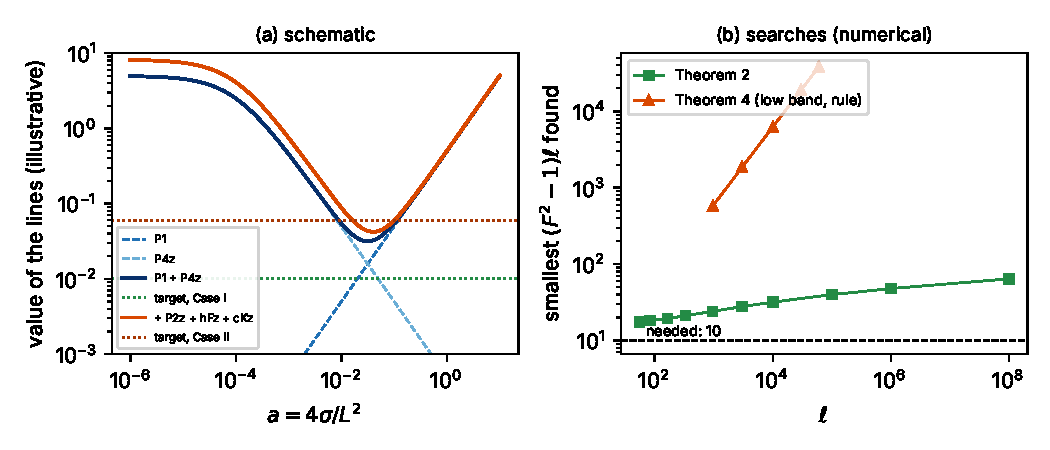
\includegraphics[width=\columnwidth]{figures/fig_cases.pdf}
\caption{(a) Schematic of the two cases of the rule, as functions of $a=4\sigma/L^2$ (log scale; illustrative values, not a state of the class). The background lines P1 and P4z have the sum $\ge\sqrt{b\omega}-\sigma/2$; in Case~I (dark ripple) it exceeds the target. In Case~II the ripple lines P2z, hFz and the chirp cKz are added. (b) The smallest $(F^2-1)\ell$ found by the searches of Sec.~\ref{sec:break}, where $F$ is the ratio of the best option to the target; the claim needs $10$. Squares: Theorem~\ref{thm:narrow}, all bands of $B$. Triangles: Theorem~\ref{thm:wide}, the band $8\ell+100\le B<5\times10^5$ (rule branch). \numst}
\label{fig:cases}
\end{figure}

\subsection{Where the hypotheses are used}

\begin{itemize}
\item No step uses a lower bound on $\mu$: small $\mu$ is handled by (m1)--(m2), where $\Theta^*$ grows like $1/\sqrt\mu$.
\item $B\ge2.5\times10^{10}$: in (R4), (b.2) and (b.5). $B\ge50(8\ell+100)$: to have $q\le0.0026$ and $z_2\le0.01$, i.e.\ coefficients of P2z and hFz close to one.
\item $a\le4r/\sigma$: in (R6)--(R7). $r\ge\sigma^3$: in (R1).
\item The boundary $\xi=\ell^2$ between (m3) and (m4) only splits the region; both are proofs of the same claim.
\end{itemize}

\subsection{The computer-assisted part}
\label{sec:ca}

The steps above are formulas.
That the $48$ quoted numbers and the $18$ conditions hold for \emph{every} $\ell\ge55.26$ is checked by interval arithmetic with outward rounding, on $[55.26,10^6]$ cut into $9{,}809$ geometric pieces of ratio $1.001$ and on the tail $[10^6,\infty)$ as one piece \caproofst{App.~\ref{app:C}}.
Functions that increase and decrease at once ($\ell^ke^{-\ell}$ and the like) are written through elementary functions whose monotonicity is proved by one derivative, so that the infinite tail gets a finite enclosure.
No piece fails.
The smallest margins are at $\ell=55.26$; for instance, Case~I with Fz has margin $0.004869$, Case~I with Tz-B2 $0.002545$, (II-ch) $0.004579$, and condition (N) $0.5845$; condition (N0) is tightest near $\ell=10^6$ with $4.93\times10^{-7}$.
The absorptions of (R1) and (R3) are a separate interval computation on $[55.26,\infty)$ as one piece: the sum of (R1) is at most $0.507288\,\mathrm{es}$ against $0.52\,\mathrm{es}$.
Table~\ref{tab:ca} lists every computer-assisted part of the paper.

The arithmetic uses Python's \code{decimal} with $40$ digits, widens every result outward by $10^{-38}$ relative, never uses the library power (which is not guaranteed to be correctly rounded in the C version), and refuses to invert an interval that contains $0$.
While the interval functions run, any rounding outside the interval context raises an exception (the \code{Inexact} flag of the default context is trapped); no exception occurs.
A test of $8{,}100$ random intervals and points against $90$-digit values finds no enclosure failure, and the same test catches each of four deliberately broken implementations.

\begin{table}
\caption{The computer-assisted parts of the paper. ``Pieces'' are intervals of $\ell$; the tail is $[10^6,\infty)$. All were run with the \code{Inexact} trap of the default context.}
\label{tab:ca}
\begin{ruledtabular}
\small
\begin{tabular}{p{0.34\columnwidth}p{0.27\columnwidth}p{0.24\columnwidth}}
what & how & code\\ \hline
48 numbers, 18 conditions of Proposition~\ref{prop:narrow} & 9,809 pieces $+$ tail & \code{dl\_consts.py}\\
absorptions (R1), (R3) & one piece $[55.26,\infty)$ & \code{dp\_r1.py}\\
constants and conditions of Proposition~\ref{prop:wide} & 6,952 pieces $+$ tail & \code{dp\_room1.py}, \code{dq\_room1\_low.py}\\
$M_4(10^{-4})\le2.0475$ (Lemma~\ref{lem:M4}) & pieces in $u$ & \code{dq\_m4.py}\\
$M_1(10^{-4})$, $M_2(10^{-4})$ (Lemma~\ref{lem:M12}) & pieces in $u$ & \code{du\_cl.py}\\
Theorem~H1 of~\cite{H} & certificates of~\cite{H} & repository of~\cite{H}\\
\end{tabular}
\end{ruledtabular}
\end{table}

\emph{Picture.}
With a narrow focus the observer sees a short piece of ripple.
If the ripple is dark, the background alone carries the information.
If it is bright, it cannot also hide at the centre of the focus; so it spreads, and its phase turns across the focus.
That turning, the chirp, is what pays.
The hardest states are where the ripple is just bright enough to need the chirp, and there the margin is $17.6/\ell$ at $\ell=55.26$, growing to $64/\ell$ at $\ell=10^8$ (Fig.~\ref{fig:cases}).

\section{Focus at the resolution (Theorem~\ref{thm:res})}
\label{sec:res}

\subsection{Statement}

\begin{proposition}[focus at the resolution, line form] \proofst
\label{prop:res}
Let $\ell\ge55.26$.
Let a state satisfy $\tfrac12<b\le1$, $\mu>0$, $\sigma^3\le r\le\tfrac14$, $\kappa>0$, and let $P>0$ satisfy (A), (K) and (CM) of Lemma~\ref{lem:Hprime}.
Then for every $a>0$ and every $\gamma\in[0,0.6]$ the lines of the option Fz satisfy $\Lambda_{\rm Fz}(a)\ge0$.
\end{proposition}

Neither (J) nor the range of $a$ is used.
The numbers below are values at $\ell=55.26$; every quantity that enters ($\varepsilon_1$, $\varepsilon_h$, $\Gamma_\ell$, $k_1$, $k_2$ and the terms with $\sigma$) decreases with $\ell$ and $\theta$ increases, so $\ell=55.26$ is the worst case.
The same numbers were also evaluated by interval arithmetic on $[55.26,\infty)$ as one piece.

\begin{proof}[Proof of Theorem~\ref{thm:res} from Proposition~\ref{prop:res}]
If $G>0$, Lemma~\ref{lem:lines} (option Fz, valid for $b\in(\tfrac12,1]$) and Proposition~\ref{prop:res} with $\gamma=0.6$ give $(a)+(a')\ge0.6$.
If $G=0$, Lemma~\ref{lem:G0} with $b\le1$ gives $(a)+(a')\ge C_0=0.1995$.
Both exceed $\Gamma_\ell\le0.1462$.
\end{proof}

\subsection{What changes when $b>\tfrac12$}

The pair lemma needs $\delta=2b/(1-b)\le2$, which fails as $b\to1$; with it go the chirp, the line hFz and the branches B1, B2, and $\mathrm{brk}=1-4b/(1-b)-z_2/12$ is negative for $b>0.2$.
The other local lemmas use only $1-b\ge0$ and $y\le10^{-4}$, and $y\le\sigma^2/4<10^{-48}$ here, where their three constants are bounded by hand (Lemma~\ref{lem:M0}); so no step of this section is computer-assisted.
So only the option Fz is available.
It is enough, because a focus this narrow sees a dark ripple: the rule would always be in Case~I ($G\le0.2943$ while $c_1\sqrt b/\Gamma_2\ge7.4$).
The option Fz does not use the pair lemma; its lower bound subtracts the positive tail line ``pair'' in addition, which only weakens it.

\subsection{Proof}

\begin{itemize}
\item[(F1$'$)] In (CM), $B_0(1/16,1)=(1+1/4+(1/32)^{1/3})^2\le2.4492$, so $P\le P_1=2[(1.5/16)\ln(32B_0(1/16,1))+c_{\rm CM}]\le0.8829$ and $G\le P_1/3\le0.2943$.
\item[(R1$'$)] N1 $=\varepsilon_1(r)$P1 with $\varepsilon_1\le0.01457$; the other L-lines are at most $e_L$P1 with $e_L\le7\times10^{-17}$; d4$+$N4G $\le\mathrm{es}_\sigma$P2z.
\item[(R2$'$)] hneg1 $=\varepsilon_h(r)$P4z, $\varepsilon_h\le0.1808$.
\item[(R3$'$)] The S-lines are at most $e_S$P4z ($a\le1$) or $e_S$P1 ($a\ge1$), $e_S\le3.1\times10^{-13}$. Put $e_2=10^{-12}\ge e_L+e_S$.
\item[(R4$'$)] $\mathrm{N3}+\mathrm{M0Xi}+\mathrm{A1v}+\mathrm{pair}\le1.86\sigma$.
\item[(R5$'$)] (K) gives $\kappa G\le\tfrac23U_1^2$ and $\sqrt\kappa\,G\le\sqrt{2P_1}U_1/3$, so $\mathrm{FzK}+\mathrm{A2k}+\mathrm{B2a}\le0.048\,\ell\sigma\le\ell\sigma$.
\end{itemize}
Hence, for every $a>0$,
\begin{equation}
\begin{split}
\Lambda_{\rm Fz}(a)\ \ge\ &(1-\varepsilon_1-e_2)\frac a2+(1-\varepsilon_h-e_2)\frac{b\omega/2}{a+\sigma}\\&+(1-\mathrm{es}_\sigma)\mathrm{P2z}+\mathrm{P3z}-\gamma bk_1-\gamma k_2G-(1.86+\ell)\sigma .
\end{split}
\end{equation}
Since $Xa+Y/(a+\sigma)\ge2\sqrt{XY}-\sigma/2$ for $X\le\tfrac12$, with $\theta=\sqrt{(1-\varepsilon_1-e_2)(1-\varepsilon_h-e_2)\omega}\ge0.8984$,
\begin{equation}
\Lambda_{\rm Fz}(a)\ \ge\ \theta\sqrt b-\gamma k_1b-\gamma k_2P_1/3-(2\ell+\tfrac12)\sigma,
\end{equation}
with $k_1\le1.0904$ and $k_2\le0.50922$.
The right side is concave in $b$, so its minimum over $[\tfrac12,1]$ is at an end.
With $\gamma=0.6$: at $b=1$ it is $0.8984-0.6542-0.0899-10^{-22}\ge0.154$, and at $b=\tfrac12$ it is $0.6353-0.3271-0.0899\ge0.218$.
$\Lambda_{\rm Fz}$ decreases in $\gamma$ (only the target lines d1--d4 contain $\gamma$), so the bound holds for all $\gamma\in[0,0.6]$.
\qed

\emph{Sharpness.}
The same proof works up to $\gamma=0.72$.
The searches of Sec.~\ref{sec:break} find the smallest $\gamma^*=0.7377$ at $\ell=55.26$, $b=1$, $r=\tfrac14$, brightness at its ceiling \numst; the proof is close to sharp.
The interval check gives $P_1\le0.882811$, $\theta\ge0.898501$ and the margins $0.15437$ ($b=1$) and $0.21831$ ($b=\tfrac12$); with $\gamma=0.75$, or without (CM), the bound at $b=1$ is negative.

\emph{Picture.}
Here the focus is only $1$ to $1.4$ times the resolution and sees less than $1/80$ of a period ($\tau\le0.006$).
At this narrowness positivity makes the ripple dark, and the two background lines, the information in $w$ and the background in $v$, carry $g\ge0.6(1-\bar\varepsilon)$, four times what the law asks.
The law is not tight here.

\section{Wide focus (Theorem~\ref{thm:wide})}
\label{sec:wide}

\subsection{Statement}

\begin{proposition}[wide focus, line form] \caproofst{App.~\ref{app:C}}
\label{prop:wide}
Let $\ell\ge960.8$.
Let a state satisfy $\mu>0$, $\sigma^3\le r\le\tfrac14$, $8\ell+100\le B<\ell^4$, $b\le\tfrac12$, $\kappa>0$, and let $P>0$ satisfy (H$'$).
Then for every $a\in(0,4r/\sigma]$ the option chosen by the rule of Sec.~\ref{sec:narrow} (same constants $c_1$, $c_T$, $c_{\rm ch}$, $a_s$) satisfies $\Lambda_k(a)\ge0$ with $\gamma=\Gamma_\ell$.
\end{proposition}

Theorem~\ref{thm:wide} follows exactly as Theorem~\ref{thm:narrow} does (Lemma~\ref{lem:lines} for $G>0$, Lemma~\ref{lem:G0} for $G=0$).
For $\ell\ge960.8$, $\ell^4\ge8.5\times10^{11}$, so the proposition overlaps Proposition~\ref{prop:narrow} and covers the band $2.5\times10^{10}\le B<50(8\ell+100)$ that Proposition~\ref{prop:narrow} leaves for $\ell>6.25\times10^7$.
The upper end $\ell^4$ is used in one step only, (b.5).

The focus is wide: $\tau=x/b\ge5\times10^{11}/B$, and the focus spans many periods.
What makes the proof of Sec.~\ref{sec:narrow} work here is that it never uses the smallness of $b$ directly.
The lower end $B\ge2.5\times10^{10}$ entered only through constants, and the lower end $B\ge50(8\ell+100)$ only through the uniform bounds $q\le0.0026$, $z_2\le0.01$.

\subsection{The lines down to $B=8\ell+100$}

For the lines to be lower bounds (Lemma~\ref{lem:lines}) we need $z_0^2\le1$, $1-q>0$ and one constant of the main-term identity, which was established for $y\le10^{-6}$ and is needed here for $y=(1-b)^2/(2B)\le1/(2(8\ell+100))<6.5\times10^{-5}$.

\begin{lemma}[the constant $M_4$] \status{(i)--(ii) proof; (iii) proof, computer-assisted}
\label{lem:M4}
Let $f(u,y)=e^{-u/2}\bigl[\tfrac{1+u}2(1+u\cosh\sqrt{yu})+\cosh\sqrt{yu}\bigr]$ and $M_4(y)=\sup_{u\ge0}f(u,y)$.
(i) The quantity $\Xi$ of the main-term identity satisfies $|\Xi|\le\Qb M_4(y)\,y$.
(ii) $M_4$ is non-decreasing in $y$.
(iii) $M_4(10^{-4})\le2.0475\le2.07$.
\end{lemma}

\begin{proof}
Put $c=\sqrt{yu}$.
(i) $1-e^{-y/2}\cosh c\le1-e^{-y/2}\le y/2$, and $e^{-y/2}\cosh c-1\le\cosh c-1\le(c^2/2)\cosh c$; so $|1-e^{-y/2}\cosh c|\le(y/2)(1+u\cosh c)$. With $ye^{-y/2}\cosh c\le y\cosh c$ the single term is at most $y f(u,y)$, and the sum over harmonics with $\sum q_n\le\Qb$ gives (i).
(ii) For fixed $u$, $\cosh\sqrt{yu}$ is non-decreasing in $y$ and enters with positive coefficients.
(iii) On $u\in[0,60]$, pieces of width $0.005$ ($[0,20]$) and $0.05$ ($[20,60]$) bound $f$ by its decreasing and increasing parts at the ends of each piece, in interval arithmetic; the largest bound is $2.04742$. For $u\ge60$, $f\le e^{-0.4987u}((1+u)^2/2+1)$, which decreases and is below $1.9\times10^{-10}$ at $u=60$.
\end{proof}

All other places where $y$ enters (the background lines, the pair lemma, the lines B1w) hold for every $y\le1$ \proofst.
So the lines are lower bounds for $B\ge8\ell+100$ with the constant $2.07$ unchanged.

\subsection{Proof: the same steps, other constants}

The steps (F), (R), Case~I, (c), (II-ch), (II-s), (m1)--(m4) of Sec.~\ref{sec:narrow} are used as they stand.
On a piece $[\ell_a,\ell_b]$ of $\ell$, with $B_m=8\ell_a+100$ the lower bound of $B$ on the piece, five constants are replaced:
\begin{itemize}
\item $q\le(1+\eta)/(8(1-\eta))$ and $z_2\le\tfrac12$ (instead of $0.0026$ and $0.01$);
\item $\mathrm{es}=0.25/B_m$ in (R1) and (R3); at $\ell=960.8$ the sum of (R1) is $0.50042\,\mathrm{es}$;
\item $e_0=2/\sqrt{B_m}+\mathrm{es}$ in (R4) ($e_0=0.022697$ at $\ell=960.8$, against $1.26\times10^{-5}$ in Sec.~\ref{sec:narrow});
\item $B_m$ inside $\omega$, $c_S$, $c_{1F}$ and $\bar\varrho$;
\item in (m4), $B<\ell^4$ closes the argument by (b.5) alone, so the conditions (N), (N0) and (F) are not used.
\end{itemize}
Some numbers of Sec.~\ref{sec:narrow} are written into the formulas and hold only for $z_2\le0.01$ or $q\le0.0026$.
They were found by reading the source line by line and replaced by arguments: $k_f\ge0.999$ in (b.5) becomes $k_f\ge(1-b)^2(1-4b/(1-b)-z_2/12)$ (with $\ell^4\sigma^2\le10^{-100}$ checked), $1/\sqrt{c_0}\ge0.999$ becomes $(m_2(1-q))^{1/4}$, the factor $2.1$ in $\mathrm{A2k}\le2.1b^2\mathrm{cKz}$ is checked as a condition (its value is $2.0915$), and three smallness claims of (II-ch), (II-s) and Case~I are checked as conditions.
Two independent counts of the written-in numbers find none missing.
At $z_2\le\tfrac12$ some constants move: in Case~I with Tz-B2, $k_f\ge0.4162$ and $\mathrm{A2k}\le0.0482\,\mathrm{cKz}$ at $\ell=960.8$.

\subsection{The computer-assisted part}

The constants and conditions are evaluated by the same interval arithmetic as in Sec.~\ref{sec:ca}, built from the source of the computation of Sec.~\ref{sec:narrow} with only the quantities above turned into arguments (with the old values it reproduces that computation to $2.2\times10^{-36}$), on $[960.8,10^6]$ cut into $6{,}952$ pieces and on the tail \caproofst{App.~\ref{app:C}}.
$35$ conditions are checked on each piece; none fails on any of the $6{,}953$ pieces.
The smallest margins are at $\ell=960.8$: Case~I with Tz-B2 $0.0023301$, Case~I with Fz $0.07874$, (II-ch) $0.038309$, and the absorption of the constant lines uses $0.96287$ of $e_0$.
Each of four deliberately wrong versions ($e_0:=\mathrm{es}$; $z_2>1$; the rule constant $c_1=0.95$; $B_m=100$) fails on all four test pieces.

\emph{Where the end $8\ell+100$ comes from.}
The constants alone go much lower: all conditions hold with $B_m=10^3$, and Case~I with Fz fails first at $B_m=300$.
The end $8\ell+100$ is the end of the lines: below $B=(8\ell+100)/2$ the ring radius $K^2=8\ell+100$ violates $z_0^2=K^2y\le1$.
The searches of Sec.~\ref{sec:break} see this: below that end the sum of the lines becomes negative for every $\gamma$, which is not a counterexample, because there the lines are not lower bounds.
This is where Theorem~\ref{thm:verywide} takes over.

\emph{Picture.}
A wide focus spans many periods, so the brightness of the ripple is spread over it ($\kappa\approx1$), and the phase turns appreciably between the centre and the edge of the focus.
The chirp gain $\chi G$ grows like $\kappa\sigma/b$, that is, like the width of the focus, and exceeds the apparent darkening of the ripple by orders of magnitude.
So the hardest states of this region are its narrowest ones, at the border with Theorem~\ref{thm:narrow}; widening the focus only helps (Sec.~\ref{sec:break}).

\section{Very wide focus (Theorem~\ref{thm:verywide})}
\label{sec:verywide}

Theorem~\ref{thm:verywide} was reduced in Sec.~\ref{sec:main} to Proposition~\ref{prop:BE} (where $\tau\ge\tau_0(\ell)=4\ln\ell+40$) and Lemma~\ref{lem:P} (everywhere).
This section proves both.
It uses neither the lines nor the brightness hypothesis.

\subsection{Proposition~\ref{prop:BE}: what changes in Lemma~BE}

Lemma~BE of~\cite{H} (\Hsec{VII}) proves $(a)+(a')\ge1.1\times10^{-5}/\sigma$ for $B\le10^4$ and $\sigma\ge10^{-3000}$ ($\ell\le6907.8$).
Its proof uses these two limits in four places only:
the numerical lower bound of $1-e$;
the comparison $\sigma^2\Jww>0.6\sigma^2\ge6\times10^{-5}b$ in the case $L^2<1$;
the value $U_1\le29.4$ of the window constant;
and the comparison of every remainder with $\sigma^2\Jww\ge0.6\sigma^3$, which needs $\tau\ge5\times10^7$.
The core of the proof, the mean-square bound of the cross term (steps BE-a to BE-3 of~\cite{H}), depends neither on $B$ nor on $\ell$.
We keep that core and change three things:
$1-e\ge y/(2+y)$ is used for general $B$;
the remainders are written as $\sigma^2$ times a ratio free of $\sigma$ and compared with the main term of each case;
and the remainder $a_4^*$ of Lemma~A4* of~\cite{H} is written as a multiple of $(1-e)W$.
Lemma~20 of~\cite{F} (narrow envelopes have $\tau>80$) is not used: $\tau\ge\tau_0(\ell)$ is a hypothesis, and Lemmas~19, 21--23 of~\cite{F} are used at that $\tau$ directly; their statements do not assume a size of $\tau$, and their remainders are written through $\nu_k(\tau,\beta)$.
Paper~H uses Lemma~R and Lemma~A4* in the same way at $\tau\ge20$.

\subsection{Proof of Proposition~\ref{prop:BE}}

Notation of~\cite{F,H}: $y=(1-b)^2/(2B)$, $e=e^{-y/2}$, $\beta=(1-b)\sqrt{\tau/(2B)}$, $\nu_k=2\sum_{n\ge1}n^ke^{-n^2\tau/2}e^{n\beta}$, $z=\Qb\nu_0/2$, $J=\sigma^2\Jww$, $\mathrm{den}=b+W+J$; $x=\tau B\sigma^2$ and $b=B\sigma^2$.

\emph{(0)} $\tau B=x/\sigma^2\ge5\times10^{11}$, hence $1/B\le\tau/(5\times10^{11})$ and $\beta\le10^{-6}\tau$.

\begin{lemma}[$\nu_k$ at moderate $\tau$] \proofst
\label{lem:nu}
If $\tau\ge60$, $\beta\le10^{-6}\tau$ and $k\le4$, then $\nu_k\le\bar\nu(\tau)=2.0000001\,e^{-0.499999\tau}$.
\end{lemma}
\begin{proof}
The ratio of the $n$-th to the first term is at most $n^4e^{-0.499999(n^2-1)\tau}$, and $\sum_{n\ge2}n^4e^{-0.499999(n^2-1)\tau}\le1.32\times10^{-38}$ for $\tau\ge60$. The first term is at most $2e^{-0.499999\tau}$.
\end{proof}

\emph{(2) The cross term (as in~\cite{H}).}
Replacing the term $-\sigma^2\gamma_P\Phi/(1-z)$ of Lemma~23 of~\cite{F} by the mean-square step with $c=(b+J)/(16\sigma^2)$ and $\Lambda=10^{-3}/\sigma^2$, the $\Phi$-part is at most $b\Psi/2+J/4$, and the curvature part is at most $\rho_W(1-e)W_{\rm per}$ plus a tail, with
\begin{gather}
\rho_W=\frac{48(1+\Qb)K_1\sigma^2}{(1-b)^2},\nonumber\\ K_1\sigma^2=\frac{10^{-3}}{1-\Qb}+\frac{\sigma^2(U_1^2+\frac12)}{(1-\Qb)^3},
\end{gather}
and $\rho_W\le0.0801$ for $\ell\ge960.8$ and $b\le(8\ell+100)\sigma^2$.
No size of $B$ is used here: the cross term costs $8\%$ of the ripple information whatever the width of the focus.

\emph{(3) $a_4^*$ as a multiple of $(1-e)W$.}
With $e\beta^2/(1-e)\le2\tau$, $e\beta/(1-e)\le2\sqrt{2\tau B}/(1-b)$ and the window constant $U_1$,
\begin{gather}
a_4^*\le\delta_4(1-e)W_{\rm per},\nonumber\\ \delta_4=\tfrac53\bigl[\tau\bar\nu+2\sqrt{2\tau B}\,\bar\nu\,\sigma\Xi/(1-b)\bigr],\nonumber\\ \Xi=\frac{U_1+\Qb e^{-1/2}}{\sqrt2(1-\Qb)}+\frac1{2\sqrt\pi}.
\end{gather}

\emph{(4) The collected inequality.}
With the sandwich $W_{\rm per}\le((1+z)W+\tfrac12b\tau\Qb\nu_2)/(1-\nu_0)$ of Lemma~22 of~\cite{F},
\begin{equation}
\begin{aligned}
2N_\phi\ \ge\ &(1-e)W\,c_1+b\Psi\,c_2-\frac J{4(1-z)}-\mathrm{rem}-(\text{tail}),\\
c_1=&\,1-\frac{\sigma^2}{(1-e)(1-\bar\nu)}-\frac{(\rho_W+\delta_4)(1+z)}{(1-z)(1-\bar\nu)},\\ c_2=&\,\frac1{1+z}-\frac1{2(1-z)},
\end{aligned}
\end{equation}
where rem is the sum of eleven remainders: $a_1,a_2,a_3,a_5,\ldots,a_{10}$ from the proof of Lemma~23 of~\cite{F}, the term proportional to $\Phi$ in its statement (with $\Phi\le2$), and the part proportional to $b$ that the sandwich brings into $\rho_W$ and $\delta_4$.
The only difference from the collected inequality of~\cite{H} is that $\delta_4$ sits in $c_1$.

\emph{(5) The remainders free of $\sigma$.}
With $x=\tau B\sigma^2$, $\sqrt x=\sigma\sqrt{\tau B}$, $b=B\sigma^2$ and $\sqrt xN_1\le U_1$, each remainder is $\sigma^2$ times a term $T_i=K_iB^{a_i}$, $a_i\in\{0,\tfrac12,1\}$, with $K_i$ a function of $\tau$ and $\ell$ (App.~\ref{app:D} lists all eleven, separated by origin).
The largest is $a_6=\nu_1(xN_1\sigma c_\chi+\sigma\sqrt x(1+\Qb)\gamma_P/\sqrt2)$, which becomes $\sqrt{\tau B}(U_1c_\chi+(1+\Qb)\gamma_P/\sqrt2)\bar\nu$; at $\ell=960.8$, $\tau=\tau_0$, $B=8\ell+100$ it is $4.12\times10^{-9}$.

\begin{lemma}[remainders] \status{proof; values checked in interval arithmetic}
\label{lem:R}
Let $\ell\ge960.8$ and $\tau\ge\tau_0(\ell)$, and let $S_R=\sum_iT_i$.
(R-2) For $0<B\le8\ell+100$: $S_R/(1-z)\le\rho_2=4.76\times10^{-9}$.
(R-1) $\mathrm{rem}/b=S_R/(B(1-z))\le\rho_1=5.49\times10^{-11}$.
\end{lemma}
\begin{proof}
Put $\bar B=8\ell+100$.
\emph{In $B$.} $B$ enters $K_i$ only through $\rho_W$ and $\delta_4$, which increase with $B$. So every $T_i$ is non-decreasing in $B$, and (R-2) is largest at $B=\bar B$. For (R-1), first bound $\rho_W$ and $\delta_4$ by their values at $\bar B$; call the result $\bar K_i$. The remaining powers of $B$ are $B^{-1}$, $B^{-1/2}$ and $1$, and $1/B\le M(\tau)=1+\tau/(5\times10^{11})$ (by (0) if $B<1$). Hence $S_R/B\le M\sum_{a_i=0}\bar K_i+\sqrt M\sum_{a_i=1/2}\bar K_i+\sum_{a_i=1}\bar K_i$.
\emph{In $\tau$.} Each term is a constant times $\tau^j\bar\nu(\tau)$ with $j\le\tfrac72$ (counting $M$ as one power of $\tau$), which decreases for $\tau\ge60$; the worst case is $\tau=\tau_0(\ell)$.
\emph{In $\ell$.} At $\tau=\tau_0(\ell)$, $\bar\nu=2.0000001\,e^{-19.99996}\ell^{-1.999996}$. The coefficients are products of $U_1c_\chi$, $\gamma_P$, $8\ell+100$, $\sqrt{8\ell+100}$ and constants, and $C(\ell)/\ell^{3/2}$ does not increase. The logarithmic derivative of each bound is at most $(-0.499996+14/67.47)/\ell<0$; the worst case is $\ell=960.8$.
\emph{Values.} At $(\ell,\tau,B)=(960.8,\,67.4711,\,7786.4)$, outward-rounded interval arithmetic gives $\rho_2\le4.76\times10^{-9}$ and $\rho_1\le5.49\times10^{-11}$.
\end{proof}

\emph{(6) The tail} of the mean-square step is below $10^{-100}J$: its ratio to $J$ is at most $89{,}300\,\Lambda^3e^{-\Lambda}$ with $\Lambda=10^{-3}e^{2\ell}$.

\emph{(7) Coefficients.} Since $2A_w\ge J$,
\begin{gather}
\mathrm{Num}\ \ge\ c_JJ+\tfrac12c_1(1-e)W+\tfrac12c_2\,b\Psi-\tfrac12\mathrm{rem},\nonumber\\ c_J=1-\frac1{8(1-z)}-10^{-100}\ge0.874999 .
\end{gather}
With $1-e\ge y/(2+y)\ge(1-b)^2/(4B+1)$ and $c_1\ge0.919999$, the coefficient of $W$ is at least $0.459/(4B+1)$.

\emph{(8) The two cases of~\cite{H}.}
If $L^2\ge1$: $\Psi\ge\min(\Phi,\tfrac12)\ge0.2211$ and (R-1) give the coefficient $\tfrac12c_2\Psi-\tfrac12\rho_1\ge0.055$ for $b$, so $\mathrm{Num}\ge\min(0.055,0.459/(4B+1))\,\mathrm{den}$.
If $L^2<1$: Lemma~21 of~\cite{F} gives $J\ge(1-\varepsilon_1)\sigma^2$ with $\varepsilon_1\le6.70\times10^{-15}$, so $b<BJ/(1-\varepsilon_1)$ and (R-2) bounds $\tfrac12\mathrm{rem}$ by $\tfrac12\rho_2J/(1-\varepsilon_1)$. Dropping $b\Psi\ge0$, the coefficient of $J$ stays above $0.874999$, and $\kappa(B)(J+b)\le0.459J/(1-\varepsilon_1)$ is paid.
In both cases $(a)+(a')\ge\kappa(B)/\sigma$.
\qed

The numbers are values of elementary functions at one point and were evaluated in interval arithmetic; what the proof needs is $\rho_1,\rho_2\le10^{-4}$ or so, and the values are below $10^{-8}$.
For $B\le10^4$ the constant $0.459/(4B+1)\ge1.147\times10^{-5}$ matches $1.1\times10^{-5}$ of Lemma~BE.

\subsection{Lemma~\ref{lem:P}: positivity and periodicity}

\begin{figure}
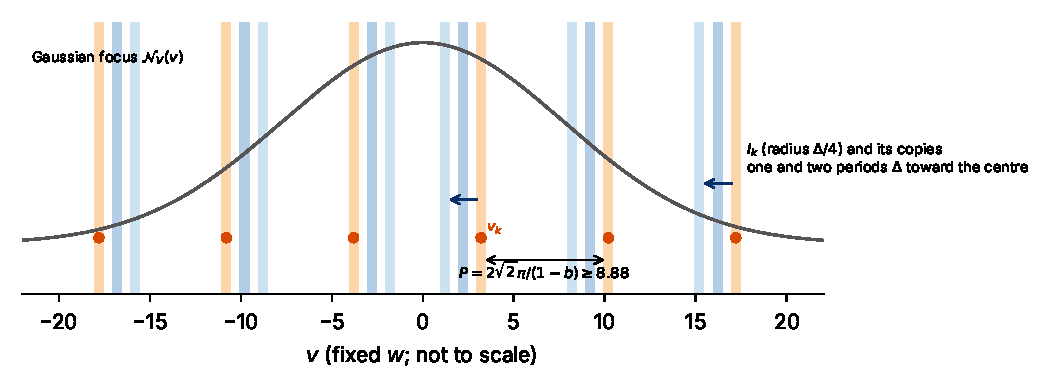
\includegraphics[width=\columnwidth]{figures/fig_lemma7.pdf}
\caption{Schematic of the proof of Lemma~\ref{lem:P} (not to scale). For fixed $w$ the phase mismatch $\phi$ vanishes only near the points $v_k$ (dots), which are $P\ge8.88$ apart. Outside the intervals $I_k$ of radius $\Delta/4$ (shaded), $\phi$ is bounded below. The weight $q=\mathcal N_V h s_v^2$ inside $I_k$ reappears one and two periods $\Delta$ closer to the centre of the focus (arrows), where $\phi$ is not small; the Gaussian focus (curve) costs at most the factor $e^{-10\pi^2/\tau}$.}
\label{fig:lemma7}
\end{figure}

\begin{proof}[Proof of Lemma~\ref{lem:P}]
If $b\ge1$ the bracket vanishes, $c_P=0$, and the claim $N_\phi\ge0$ is clear because the integrand is non-negative. Let $0<b<1$.

We have $N_\phi=(\sigma^2/2)\iint p\,s_v^2\phi$, $\phi=1-\cos m_z\ge0$, $\sqrt2m_z=v+\sigma^2s_v+w+\sigma^2s_w$, with $s_v=-v/V+k'h_t/h$ and $s_w=(\ln\Gamma)'(w)+h_w/h$ ($=-w/L^2+h_w/h$ for $\Gamma=N(0,L^2)$).
The integrand is non-negative.

\emph{The phase.}
Since $\sigma^2s_v=-bv+\sigma\sqrt x\,h_t/h$,
\begin{gather}
\sqrt2m_z=(1-b)v+c(w)+\varepsilon(v,w),\nonumber\\ c(w)=w+\sigma^2(\ln\Gamma)'(w),\qquad \varepsilon=\sigma\sqrt x\frac{h_t}h+\sigma^2\frac{h_w}h .
\end{gather}
The proof uses about $\Gamma$ only that, for fixed $w$, $c(w)$ is a number independent of $v$.
Since $|\sigma\sqrt xh_t/h|\le\sigma\sqrt xN_1/(1-\Qb)$ and $|\sigma^2h_w/h|\le\sigma^2(|w|/s^2)e^{-w^2/2s^2}\Qb/(1-\Qb)\le\sigma\Qb e^{-1/2}/(1-\Qb)$ (using $s\ge\sigma$), we have $|\varepsilon|\le\sigma a$.

\emph{Fix $w$.}
Let $v_k=(2\sqrt2\pi k-c(w))/(1-b)$, $k\in\mathbb Z$, $r=\Delta/4$, $I_k=(v_k-r,v_k+r)$ and $I=\bigcup_kI_k$.
The spacing is $P=2\sqrt2\pi/(1-b)\ge2\sqrt2\pi>8.88$ because $0<1-b<1$.

\emph{(i) Outside $I$, $\phi$ is bounded below.}
For $v\notin I$ the distance of $(1-b)v+c(w)$ to $2\sqrt2\pi\mathbb Z$ is at least $(1-b)r$, so the distance of $m_z$ to $2\pi\mathbb Z$ is at least $((1-b)r-\sigma a)_+/\sqrt2$.
With $1-\cos u\ge2u^2/\pi^2$ on $|u|\le\pi$,
\begin{equation}
\phi\ \ge\ \phi_r=\frac{((1-b)r-\sigma a)_+^2}{\pi^2}=\frac{\sigma^2}{4x}\Bigl((1-b)-\frac{2a\sqrt x}\pi\Bigr)_+^2 .
\end{equation}

\emph{(ii) The weight inside $I$ is also outside.}
Let $q(v)=\mathcal N_V(v)h(k'v,w)s_v(v,w)^2\ge0$.
Fix $k$, let $\epsilon_k=\mathrm{sgn}(v_k)$ ($+1$ if $v_k=0$), $v\in I_k$, and $u_j=v-j\epsilon_k\Delta$, $j=1,2$: one and two periods towards the centre of the focus.
Because $h$ and $h_t$ have period $2\pi$ in $t=k'v$ and $k'\Delta=2\pi$, they take the same values at $u_j$ and at $v$, while $s_v(u_j)=s_v(v)+jd$, $d=\epsilon_k\Delta/V$.
The Gaussian ratio is $\mathcal N_V(u_j)/\mathcal N_V(v)=\exp(j\Delta(2\epsilon_kv-j\Delta)/(2V))$; since $\epsilon_kv\ge|v_k|-r\ge-\Delta/4$, the exponent is at least $-j(j+\tfrac12)\Delta^2/(2V)\ge-\tfrac52\Delta^2/V=-10\pi^2/\tau$ for $j\le2$ (because $\Delta^2/V=4\pi^2/\tau$).
Moreover $(s+d)^2+(s+2d)^2\ge s^2/5$ for all $d$ (the minimum is at $d=-3s/5$).
Hence $q(u_1)+q(u_2)\ge e^{-10\pi^2/\tau}q(v)/5=\theta q(v)$, and integrating over $v\in I_k$,
\begin{equation}
\int_{I_k-\epsilon_k\Delta}q+\int_{I_k-2\epsilon_k\Delta}q\ \ge\ \theta\int_{I_k}q .
\end{equation}
The shifted intervals have centres at distance $\Delta$ and $2\Delta$ from $v_k$ and radius $\Delta/4$; they are disjoint from each other and from $I_k$.
All lie within $2\Delta+\Delta/4$ of $v_k$, and $2(2\Delta+\Delta/4)=4.5\Delta<8.88\le P$ for $\Delta\le1$, so they meet no other $I_{k'}$ and no shifted interval of another $k$ (whatever its direction).
All lie outside $I$.
Summing over $k$: $\int_{I^c}q\ge\theta\int_Iq$, that is $\int_{I^c}q\ge\frac\theta{1+\theta}\int q$.

\emph{Conclusion.}
$\int q\phi\,dv\ge\phi_r\int_{I^c}q\ge\phi_r\frac\theta{1+\theta}\int q\,dv$.
Multiplying by $\Gamma(w)/Z$ and integrating over $w$ gives $\E[s_v^2\phi]\ge\phi_r\frac\theta{1+\theta}\Jvv$, so
$N_\phi\ge\frac{\sigma^2}{8x}\frac\theta{1+\theta}((1-b)-2a\sqrt x/\pi)_+^2\,\sigma^2\Jvv$, and $\sigma^2\Jvv=b+W$ by Lemma~22 of~\cite{F}.
\end{proof}

The constant is loose on purpose.
The true $N_\phi/(b+W)$ is of size $1/(8B)$ \numst, and $c_P$ is smaller than that by about $\tau$; the law needs only the size $\sigma$.
In the class, $\Delta\le2\pi/\sqrt{5\times10^{11}}<10^{-5}$, far inside the condition $\Delta\le1$.
Moving the weight three or more periods may improve $\theta$, at the price of a stronger disjointness condition and a faster Gaussian decay; the theorem does not need it, and we have not tried.

\emph{Picture.}
Over hundreds of periods the observer no longer sees single ripples but their average brightness.
The information that reaches her is the slope information of the ripple times the phase mismatch between the centre and the edge of the focus, and the mismatch is as large as the focus is wide: the information is of size $1/(B\sigma)$, which exceeds what the law asks by a factor of order $e^\ell$.
The cross term between curvature and mismatch, measured over the whole ripple rather than at its worst point, takes $8\%$ of it.
When the focus spans only a few periods the average is not available, but the ripple repeats.
A steep slope hidden where the mismatch happens to vanish is present again one period and two periods away, where it does not vanish; it is dimmer there, in the tail of the focus, but brightness is never negative, so it is only discounted, never cancelled.

\section{Attempts to break the claims}
\label{sec:break}

Every claim of this paper was attacked numerically before its proof was written, following a search plan fixed in advance.
For each claim we report the families searched, planted adversaries (``dips'' of known depth placed in the space of states, which the search must find), and deliberately wrong versions of the claim, which the same search must break.
A search that finds the planted dips and breaks the wrong versions has shown that it can see a failure; a search that finds nothing without this check shows little.
All statements of this section are \numst; none of them is used in a proof.
Table~\ref{tab:break} summarizes them.

\begin{table*}
\caption{Attempts to break the claims. ``Margin'' is the smallest value found of the quantity in the second column (the claim needs the value in brackets). ``Power'' lists deliberately wrong versions and how many of them the same search broke. All entries are \numst.}
\label{tab:break}
\begin{ruledtabular}
\small
\begin{tabular}{p{0.14\textwidth}p{0.18\textwidth}p{0.16\textwidth}p{0.19\textwidth}p{0.19\textwidth}}
claim & quantity [needed] & margin & families & power\\ \hline
Theorem~\ref{thm:narrow} (lines) & $(F^2-1)\ell$ of the best option [$10$] & $17.5547$ ($\ell=55.26$) to $64.0750$ ($\ell=10^8$) & 13 families, 10 values of $\ell$, $4.8\times10^4$--$1.3\times10^5$ states each & 12 planted dips found; 8 wrong versions broken (a line dropped, (J) dropped, one option only)\\
the rule of Sec.~\ref{sec:narrow} & $(F^2-1)\ell$ of the rule [$10$] & $17.5565$ ($\ell=55.26$), no state below & 4 values of $\ell$, 7{,}200--7{,}503 states each & ---\\
Theorem~\ref{thm:res} (lines) & $\gamma^*$ [$0.6$] & $0.7377$ ($\ell=55.26$, $b=1$) & 6 values of $\ell$, about 23{,}500 points each & planted dip found; P1, P4z or (CM) dropped: broken; claim $\gamma^*\ge0.8$: broken\\
Theorem~\ref{thm:wide} (lines) & $(F^2-1)\ell$ of the rule [$10$] & $576.3$ ($\ell=960.8$, $B=8\ell+100$) & 13 families $+$ wide-focus families, $\ell$ up to $10^9$ & 7 planted dips found; cKz, P1 or (J) dropped, one option only: broken\\
Proposition~\ref{prop:BE} & $((a)+(a'))\sigma/\kappa(B)$ [$1$] & $3.56$ (197 states); $1.21$ (24 planted tight states) & true quantity, $\ell=6,8,10$ & $0.459\to0.6,0.75,1.0$: broken in 6, 14, 20 states; $(1-e)\to1$: 42; $\Psi\to1$: 27\\
Lemma~\ref{lem:R} & remainders [$\le2\times10^{-4}$] & $4.76\times10^{-9}$ & 10{,}245 points of $(\ell,\tau,B)$ & $\tau_0=2\ln\ell+10$: $\ge8.40$; $\nu\sim e^{-\tau/4}$: $\ge0.100$\\
Lemma~\ref{lem:P} & $N_\phi/(c_P(b+W))$ [$1$] & $1{,}482$ (117 states); $1{,}683$ (20 states, non-Gaussian $\Gamma$) & true quantity, $\ell=6,8$, $\tau$ from $0.06$ to $1800$ & $\theta\to\frac15$: broken in 2 states (8 with non-Gaussian $\Gamma$)\\
steps of Lemma~\ref{lem:P} & $\phi/\phi_r$; $\int_{I^c}q/(\theta\int_Iq)$ [$1$] & $2.46$; $39.6$ & 45 states $\times$ 11 values of $w$ & $\phi_r\times4$: broken in all 45; $\theta\to\frac15$: 3\\
\end{tabular}
\end{ruledtabular}
\end{table*}

\subsection{The lines (Theorems~\ref{thm:narrow}--\ref{thm:wide})}

\emph{What is searched.}
The claims of Propositions~\ref{prop:narrow}, \ref{prop:res} and~\ref{prop:wide} are statements about the sums of lines over the whole state space allowed by (H$'$): $\mu\in[e^{-3\ell},8\ell+80]$, $r\in[\sigma^3,\tfrac14]$, $\kappa\in[e^{-2.2\ell-50},e^{3\ell}]$, $B$ in its band, and $P$ up to the ceiling of (H$'$).
$F$ denotes the ratio of the lines' value to the target, and the claim $\Lambda\ge0$ with $\gamma=\Gamma_\ell$ is $(F^2-1)\ell\ge10$.

\emph{Results.}
For Theorem~\ref{thm:narrow} the smallest value is $17.5547$ at $\ell=55.26$ and grows slowly with $\ell$ (Fig.~\ref{fig:cases}b).
It sits in every case at the same corner: $\mu\approx\ell/4-\delta$, $r\approx\sigma^{1/2}$, $b\approx\sigma$, the brightness at its ceiling, and the option Tz-B1.
For Theorem~\ref{thm:res} the smallest $\gamma^*$ is $0.7377$, at $b=1$, $r=\tfrac14$ and the brightness at its ceiling, and no state of Case~II exists there.
For Theorem~\ref{thm:wide} the smallest value of the rule's branch is $576.3$ at $\ell=960.8$ and $B=8\ell+100$, far above $10$; the best option gives at least $2.16\times10^5$ in this band.
The rule's branch is smallest where the rule switches from Case~I to Case~II; this is set by the rule constant $c_1$, not by a hard state.

\emph{Power.}
Dropping any of the lines P1, P2z, hFz, P4z or cKz, dropping (J) from (H$'$), or keeping only Fz or only Tz-B2, breaks Theorem~\ref{thm:narrow} at $\ell=55.26$ and $955.8$.
Some versions are not broken: the option Tz-B1 alone suffices numerically, and removing the lower end of $b$ or either end of $a$ does not break the claim.
The proof uses those ends, but they are not numerically necessary.
At $\ell=955.8$ (not at $55.26$), the pairs $\lambda\approx1$ of (J) are needed.
The planted dips of depth $5$ at the corner, at narrow states and at low $\mu$, each with two widths and at $\ell=165.78$ and $10^5$, are all found.
The first version of the search missed four of them, because only the 40 globally lowest points were refined; the search was changed to refine the best point of every family.

\emph{The lines against the lemmas.}
That each line is a lower bound for the term of the lemma it comes from was audited in $64$ to $84$ decimal digits at $12$ values of $\ell$ from $55.26$ to $10^{12}$ ($1{,}500$ states each), with no violation; deliberately altered lines are caught.
The $30$ groups of formulas behind the lines were checked step by step at $37{,}886$ points, with no failure.

\subsection{The very wide focus (Theorem~\ref{thm:verywide})}

\emph{The true quantities.}
For Proposition~\ref{prop:BE} and Lemma~\ref{lem:P} we compare with the true $(a)+(a')$ and $N_\phi$ computed by direct two-dimensional quadrature, with the $v$-grid following the highest harmonic up to $200{,}001$ points.
Double precision reaches only $\sigma=e^{-\ell}$ with $\ell\le10$, where the regime $x\ge5\times10^{11}\sigma^2$ cannot hold.
These comparisons test the formulas at small $\ell$; they are evidence about the formulas, not about the theorems.
For Proposition~\ref{prop:BE} we impose $B\ge200/\tau$, i.e.\ $\beta\le0.05\tau$, as the small-$\ell$ analogue of $\beta\le10^{-6}\tau$.

\emph{Results.}
On $197$ states ($B\in[0.16,300]$, $\tau\in[40,1500]$, one to five harmonics, envelopes at the ends and in the middle of the class) the ratio $((a)+(a'))\sigma/\kappa(B)$ is at least $3.56$, and the collected inequality of the proof holds in all of them (Fig.~\ref{fig:true}).
\emph{A wrong expectation.}
We expected the version with $0.459$ replaced by $0.6$ to break where the ripple dominates.
It did not, because a wide envelope makes the term $eW\Phi$ that the proof drops large.
We then planted $24$ states where the bound should be tight (narrow envelope $L^2=c/B$, one strong high harmonic, $W/b$ of $3{,}000$ to $6{,}000$, $\ell=10$): the ratio is at least $1.21$, and the versions with $0.6$, $0.75$ and $1.0$ break in $6$, $14$ and $20$ of them.
The constant $0.459$ has about $20\%$ room where we can measure it.
For Lemma~\ref{lem:P} the bound has a large margin ($1{,}482$ and more); its steps (i) and (ii) were checked separately at fixed $w$.
The steps hold with margins $2.46$ and $39.6$; the minimum of $\phi/\phi_r$ is close to $\pi^2/4$, which is the gap between $1-\cos u\ge2u^2/\pi^2$ and $u^2/2$.
Measured directly, $N_\phi\cdot8B/(b+W)\ge1.000$ for $B\ge3$, so the true $N_\phi$ is close to $(b+W)/(8B)$ \numst.

\begin{figure}
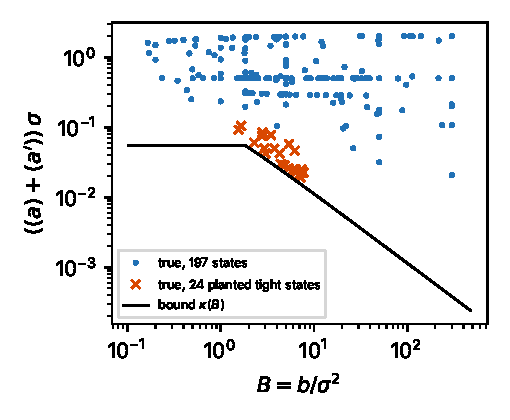
\includegraphics[width=\columnwidth]{figures/fig_true.pdf}
\caption{Proposition~\ref{prop:BE} against the true quantity, by direct quadrature at $\ell=6,8,10$ (material, outside the regime of the theorem). Dots: $((a)+(a'))\sigma$ for the 197 states with $\tau\ge40$ and $B\ge200/\tau$. Crosses: the 24 planted tight states. Line: the bound $\kappa(B)=\min(0.055,0.459/(4B+1))$. \numst}
\label{fig:true}
\end{figure}

\emph{Picture.}
The searches look in every corner of the space of states and find the hardest point of each claim, and in every case it lies above what the law asks.
The hardest states are always of the same kind: the ripple is as bright as positivity allows, and it sits where the focus is about to stop helping.

\section{Limits and outlook}
\label{sec:limits}

\subsection{The status of every statement}

Table~\ref{tab:status} lists every statement used for Theorem~\ref{thm:main} with its status and origin.
Two of the five theorems are proofs in the strict sense; Theorems~\ref{thm:narrow}, \ref{thm:wide} and Theorem~H1 of~\cite{H} are computer-assisted, so Theorem~\ref{thm:main} is computer-assisted.
It assumes condition (P6) through the factor $1-\bar\varepsilon$.

\begin{table*}
\caption{Every statement of the chain, with its status and origin. ``Borrowed'' statements are proved in the cited paper and used as stated there.}
\label{tab:status}
\begin{ruledtabular}
\small
\begin{tabular}{p{0.42\textwidth}p{0.2\textwidth}p{0.26\textwidth}}
statement & status & origin\\ \hline
$g\ge(1-|\varepsilon|)((a)+(a'))$, $|\varepsilon|\le\bar\varepsilon$ & proof, assuming (P6) & borrowed: \cite{F}, Eq.~(3)\\
Lemmas 19, 21--23 of~\cite{F} (period averages) & proof & borrowed: \cite{F}, App.~D\\
Lemmas CM-1, CN-1 (second line), R$_\theta$, A4*, the steps of BE; window constants & proof & borrowed: \cite{H}, \Hsecs{III, VI, VII, IX~A}\\
Theorem~H1 & proof, computer-assisted & borrowed: \cite{H}, \Hsec{VIII}\\
Lemma~\ref{lem:lines} (the lines; local lemmas of App.~\ref{app:A}) & proof for $y\le10^{-40}$; for $y\le10^{-4}$ the constants $M_1$, $M_2$, $M_4$ computer-assisted & new\\
Lemma~\ref{lem:M12} & (i) proof; (ii) computer-assisted & new\\
Lemma~\ref{lem:M0} & proof & new\\
Lemma~\ref{lem:Hprime} (brightness hypothesis) & proof & new (uses CM-1, CN-1)\\
Lemma~\ref{lem:DI} (closed forms, $E_J$) & proof & new\\
Lemma~\ref{lem:G0} ($G=0$) & proof & new\\
Proposition~\ref{prop:narrow}, Theorem~\ref{thm:narrow} & proof, computer-assisted & new\\
Proposition~\ref{prop:res}, Theorem~\ref{thm:res} & proof & new\\
Lemma~\ref{lem:M4} & proof; (iii) computer-assisted & new\\
Proposition~\ref{prop:wide}, Theorem~\ref{thm:wide} & proof, computer-assisted & new\\
Lemmas~\ref{lem:nu}, \ref{lem:R}, Proposition~\ref{prop:BE} & proof (values checked in interval arithmetic) & new (core from Lemma~BE)\\
Lemma~\ref{lem:P} & proof & new\\
Theorem~\ref{thm:verywide} & proof & new\\
Theorem~\ref{thm:main} & proof, computer-assisted, assuming (P6) & new\\
everything in Sec.~\ref{sec:break} & numerical & new\\
\end{tabular}
\end{ruledtabular}
\end{table*}

\subsection{What is not covered}

\begin{itemize}
\item \emph{Windows with a stronger ripple.} Theorem~\ref{thm:main} assumes $\eta\le1/\ell$, which enters Theorems~\ref{thm:narrow}--\ref{thm:wide} through the sandwich factors $1/(1\pm\eta)$ written into the lines and Theorem~H1 through its item~(i). Theorem~\ref{thm:verywide} does not need it, so the very wide focus is settled for every window of the class. In the other regions, windows with $\eta>1/\ell$ are outside this paper, except for those covered by items (ii)--(iii) of Theorem~H1 of~\cite{H} at $\tau\ge20$ and $\ell\le960.8$.
\item \emph{The class constant.} Every bound on $g$ carries $1-\bar\varepsilon$ from (P6). Its value for band windows is open (the third-order terms~\cite{H}). Our statements on $(a)+(a')$ do not depend on it.
\item \emph{The regime.} We work in $5\times10^{11}\sigma^2\le x\le0.003$. Larger $x$ is covered by Theorem~48 of~\cite{F} (for $\sigma\le10^{-24}$); smaller $x$ is not treated here. The lower end is used through the window constant $U_1$ and, in Theorem~\ref{thm:verywide}, through $\tau B\ge5\times10^{11}$.
\item \emph{Moderate resolution.} For $55.26\le\ell<960.8$ and $B<2.5\times10^{10}$ the bound is that of Theorem~H1, $g\sqrt\ell\ge1-\bar\varepsilon$, without the factor $\sqrt{1+10/\ell}$.
\item \emph{The upper side.} The law has two sides; this paper extends only the lower one. The upper side is that of~\cite{F}.
\item \emph{Computer assistance.} Theorems~\ref{thm:narrow} and~\ref{thm:wide} rely on finitely many interval-arithmetic evaluations (Table~\ref{tab:ca}). They can be rerun with the code that accompanies the paper, and they rest on the correctness of the arithmetic described in Sec.~\ref{sec:ca} and App.~\ref{app:C}. The certificates of Theorem~H1 rely on the assumption that the floating-point elementary functions (log, exp, log1p, expm1 and the square root) are accurate to within 2 ulp; the assumption and the measured errors (at most 0.71 ulp) are stated in App.~E of~\cite{H}. The computer-assisted parts of this paper do not use this assumption: they are decimal interval arithmetic with outward rounding, and the double-precision evaluations in the accompanying code are numerical checks only.
\item \emph{Numerical evidence at small $\ell$.} The comparisons with the true quantities (Sec.~\ref{sec:break}) are at $\ell\le10$; in the range of the theorems only the proofs speak.
\end{itemize}

\subsection{Outlook}

\begin{itemize}
\item \emph{Sharper constants.} The proof of Theorem~\ref{thm:res} reaches $\gamma=0.72$ against the numerical $0.7377$; a joint treatment of $P_1$, $k_1$ and $k_2$ might close the gap. The constant $0.459$ of Proposition~\ref{prop:BE} is within about $20\%$ of the states we can measure.
\item \emph{Lemma~\ref{lem:P} with more periods.} Moving the hidden weight three or more periods may improve $\theta=e^{-10\pi^2/\tau}/5$, at the cost of a stronger disjointness condition and a faster Gaussian decay. The theorem does not need it.
\item \emph{The true size of $N_\phi$.} The measurements suggest $N_\phi\ge(b+W)/(8B)$ up to a factor close to one \conjst; a proof would make Lemma~\ref{lem:P} sharp.
\item \emph{Windows with a stronger ripple} \status{outlook, not a claim}. Every window of the class has $\eta\le\Qb=\frac14$, so its sandwich factors satisfy $\lambda/\Upsilon=(1-\eta)/(1+\eta)\ge\frac35$. Theorem~\ref{thm:verywide} does not use $\eta\le1/\ell$, and items~(ii) and~(iii) of Theorem~H1 of~\cite{H} already hold with the factor $\lambda/\Upsilon$ in place of $\eta\le1/\ell$. For Theorem~\ref{thm:res}, an estimate in floating point with $\eta=\frac14$ in every line leaves a margin of about $0.50$ with the target coefficient one (at $b=1$, $\ell=55.26$) \numst. For Theorems~\ref{thm:narrow} and~\ref{thm:wide}, the sandwich factors of the gains and of the denominator cancel against the target $\lambda/\Upsilon$, but five places do not: the background remainders $\varepsilon_1$ and $\varepsilon_h$, the factor $k_1$ of the denominator, the factors $1/(1-\eta)$ on the side of the losses, and one step of the group FrB1, which fails at $\eta=\frac14$ unless the coefficient $X_1$ is enlarged. The rule constants $c_1$, $c_T$ and $c_{\rm ch}$ then have to be chosen again; in the same estimate the main conditions keep positive margins with $c_1\approx0.62$, $c_T\approx6.5$ and $c_{\rm ch}\approx1.7$ \numst. If the lines are rewritten with the remainders bounded uniformly at $\eta=\frac14$ and the sandwich factor $\lambda$ only on the main gains, each line is affine in $\lambda$, and the scaling step of~\cite{H} would give every $\lambda\in[\frac35,1]$ from the two ends $\lambda=1$ and $\lambda=\frac35$. This would give the law with coefficient $\lambda/\Upsilon\ge\frac35$ for every window of the class. It is work for a later paper; nothing in this item is claimed.
\item \emph{Towards general states} \status{outlook, not a claim}. Paper~F splits Conjecture~1 of Paper~E into three cases (Theorem~16 of~\cite{F}, the case split). Cases~1 and~2 are proved there; Case~3 is reduced to Conjecture~18 of~\cite{F}, the visibility inequality $\keff^2\le\frac12\ln(1/Q)+C$, which with a floor $Q\ge\sigma^2/C$ would give Conjecture~1 with constant $\frac12$. In Case~3, by the localisation Lemma~17 of~\cite{F}, $\E_{\pi_v}[d(m_z)^2]\le(\pi^2/2)\theta=(\pi^2/8)QW_2$: the slope information hides near the points where the phase mismatch vanishes, within a root-mean-square distance $\ll\sqrt{W_2/\ls}$. Lemma~\ref{lem:P} handles exactly this hidden weight for periodic windows, and carries it outward by positivity and periodicity; both arguments rest on the same inequality $1-\cos t\ge(2/\pi^2)d(t)^2$, with $d(t)$ the distance to $2\pi\mathbb Z$. In states whose ripple does not repeat, a replacement for the shift by one period would bring Conjecture~18 closer. Lemma~CM-1 of~\cite{H} (\Hsec{IX~A}), $xE_1\le(1+b/2)E_0\ln(2B_0/E_0)+(\sqrt2/e)bE_0'$, bounds the square of the local wavenumber, $\mu=xE_1/E_0$, by the logarithm of the inverse brightness, the same shape as Conjecture~18; its proof uses only $f\ge0$, the analytic continuation of the Gaussian-blurred profile and Paley--Wiener. Extending that method to two-dimensional general states, and the outward shift of Lemma~\ref{lem:P}, are two candidate tools for Conjecture~18. Nothing in this item is claimed.
\end{itemize}

\emph{Picture.}
The map of states is closed for windows with a weak ripple: wherever the observer focuses and however fine her lens, the information that survives the blur is at least the fraction $(1-\bar\varepsilon)/\sqrt\ell$.
What remains open is not a region of the map but the shape of the windows: how strong a ripple the law tolerates, and how small $\bar\varepsilon$ is.


\begin{acknowledgments}
The author used AI assistants in this work. Anthropic Claude was used in two separate sessions. The first session (claude-opus-5-5) wrote the instructions for each stage, re-ran every verification suite in a fresh folder, recomputed the key constants by hand, and reviewed the manuscript. The second session derived the lemmas and the proofs of Theorems 2 to 5, wrote the interval arithmetic and the verification code, and drafted the text, using Anthropic Claude Fable (claude-fable-5-2) for the new proof ideas, among them the narrow-focus lemmas and the positivity-and-periodicity lemma (Lemma 7), and claude-opus-5-5 otherwise; it also found constants that had been left as numerical maxima and closed them by proofs. Google Gemini (Gemini 4 Argon) and OpenAI ChatGPT (GPT-6 Sol) independently reviewed the manuscript; their comments led to the lower end of the borrowed Lemma BE and several corrections of notation.
The author directed the research, made all decisions on its content, and takes full responsibility for this article.
\end{acknowledgments}

\emph{Data and code availability.}
All code, stored results, the interval-arithmetic computations and the verification suite are available at \url{https://github.com/neginyan/resolution-gap-every-focus} and archived at Zenodo (DOI added on publication).
A single entry point, \code{verification/run\_all.py}, recomputes every computer-assisted part of this paper and re-derives its numbers from the stored results; \code{verification/quick.py} is a short check that runs in a few minutes.
The certificates of Theorem~H1 are those of~\cite{H} and are re-run with the repository of~\cite{H}.
Paper~F and its repository~\cite{F} are not changed; this paper uses version~1.3 of paper~H~\cite{H}, prepared together with it.


\appendix
\section{The local lemmas and the brightness lemmas}
\label{app:A}

This appendix proves the lemmas behind Lemmas~\ref{lem:lines}--\ref{lem:G0} and states the lemmas borrowed from~\cite{F,H} in the form in which they are used.
Sections~\ref{app:A:not}--\ref{app:A:sum} are the local lemmas (new); Sec.~\ref{app:A:w} is the $w$-branch of Lemma~R$_\theta$ of~\cite{H} as it enters the lines; Secs.~\ref{app:A:J}--\ref{app:A:G0} are the brightness lemmas and the states with $G=0$ (new); Sec.~\ref{app:A:borrowed} lists the borrowed statements and compares them with the published text and code.

\subsection{Notation}
\label{app:A:not}

A state is $p=\mathcal N_V(v)\,\Gamma(w)\,h(t,w)/Z$ with $t=k'v$, $h=1+E\,R$, $E=e^{-w^2/(2s^2)}$, $R(t)=\sum_nq_n\cos(nt-\phi_n)$, $V=\sigma^2/b$, $\Gamma=N(0,L^2)$, $x=(k'\sigma)^2$, $\tau=x/b$, $y=(1-b)^2\sigma^2/(2b)=(1-b)^2/(2B)$ and $r=s^2/L^2$.
On the line, $\hat s\sim N(0,1)$ and $t=t_0+\sqrt\tau\,\hat s$; $\E_\rho$ is the average over $\hat s$, and $\langle\cdot\rangle=\int\Gamma(w)\,dw\,\E_\rho[\cdot]$.
We write
\begin{gather}
X_1=\sqrt x\,R'(t),\quad \tilde F=E^2X_1^2/h\ge0,\nonumber\\ u=\sqrt y\,\hat s,\quad v=w/\sqrt2,\quad a=u+v,\nonumber\\
\chi=\chi_v+\chi_w,\quad \chi_v=\frac{\sigma EX_1}{\sqrt2\,h},\nonumber\\ \chi_w=-\frac{\sigma^2w}{\sqrt2}\Bigl(\frac1{L^2}+\frac{ER}{s^2h}\Bigr),
\end{gather}
$k_E=\sqrt{r/(1+r)}$, $\mathrm{se}_E=s^2/(1+r)$, $e_E=e^{-\mathrm{se}_E/4}$, $g_s=\sqrt{r/(2+r)}$, $\mathrm{se2}=s^2/(2+r)$, $E_0=\E_\rho[R^2]$, $E_1=\E_\rho[R'^2]$, $P=2xE_1$, $W=xg_sE_1=G/2$, $\kappa=\E_\rho[\hat s^2R'^2]/E_1$, $\eta=\sup|R|$, $U=\sup|X_1|$ (in the class $\eta\le1/\ell$, $U\le U_1$, $\sum q_n\le\Qb=\tfrac14$), $R_\theta=\E_\rho[R]=\sum_nq_ne^{-u_n/2}\cos\phi_n$, $t_\rho=-x\E_\rho[R'']=b\sum_nu_nq_ne^{-u_n/2}\cos\phi_n$ with $u_n=n^2\tau$, and $T_2(K)=\E[\hat s^21\{|\hat s|>K\}]=2(K\varphi(K)+Q(K))$ with $\varphi$, $Q$ the standard normal density and upper tail.
The averages over $w$ used below are
\begin{gather}
\textstyle\int\Gamma E=k_E,\ \int\Gamma E\cos v=k_Ee_E,\ \int\Gamma E^2=g_s,\nonumber\\
\textstyle\int\Gamma E^2\cos v=g_se^{-\mathrm{se2}/4},\ \int\Gamma E^2w^2=g_s\mathrm{se2},\nonumber\\
\textstyle\int\Gamma E^2|w|=g_s\sqrt{2\mathrm{se2}/\pi},\ \int\Gamma E|w|=k_E\sqrt{2\mathrm{se}_E/\pi},\nonumber\\
\textstyle\int\Gamma Ew^2=k_E\mathrm{se}_E,\ \int\Gamma|w|=L\sqrt{2/\pi}.
\end{gather}
Three Gaussian facts are used repeatedly: Stein's identity $\E[\hat sg(\hat s)]=\E[g'(\hat s)]$, and, for real $\alpha$ and $\phi$,
\begin{gather}
\E[\cos(\alpha\hat s-\phi)]=\cos\phi\,e^{-\alpha^2/2},\nonumber\\ \E[\hat s\sin(\alpha\hat s-\phi)]=\alpha\cos\phi\,e^{-\alpha^2/2},\nonumber\\
\E[\hat s^2\cos(\alpha\hat s-\phi)]=(1-\alpha^2)\cos\phi\,e^{-\alpha^2/2}.
\label{eq:gauss3}
\end{gather}
(The second is Stein's identity applied to the first; the third is Stein's identity applied to $g=\hat s\cos(\alpha\hat s-\phi)$.)

\subsection{The direct form of the $v$-branch}

\begin{lemma}[direct form] \proofst
\label{lem:CZ1}
$Z\sigma^2\E_p[s_v^2\phi]=\langle hS^2(1-\cos(a+\chi))\rangle$ with $S=\sqrt b\,\hat s-EX_1/h$. Expanding $hS^2=b\hat s^2h-2\sqrt b\,\hat sEX_1+\tilde F$,
\begin{gather}
Z\sigma^2\E_p[s_v^2\phi]=\mathrm{(I)}+\mathrm{(II)}+\mathrm{(III)},\nonumber\\
\mathrm{(I)}=b\langle\hat s^2h(1-\cos(a+\chi))\rangle,\nonumber\\ \mathrm{(II)}=-2\sqrt b\langle\hat sEX_1(1-\cos(a+\chi))\rangle,\nonumber\\
\mathrm{(III)}=\langle\tilde F(1-\cos(a+\chi))\rangle .
\end{gather}
\end{lemma}
\begin{proof}
$s_v=\partial_v\ln p=-v/V+k'ER'/h$. With $v=\sqrt V\hat s$, $\sigma/\sqrt V=\sqrt b$ and $\sigma k'=\sqrt x$ this is $\sigma s_v=-S$.
The phase of $\phi=1-\cos m_z$ is $m_z=(v+\sigma^2s_v+w+\sigma^2s_w)/\sqrt2$ with $s_w=-w/L^2-(w/s^2)ER/h$; the part $v+\sigma^2s_v$ is $\sqrt2(u+\chi_v)$ and the part $w+\sigma^2s_w$ is $\sqrt2(v+\chi_w)$, so $m_z=a+\chi$.
Nothing else is used; the lemma is the definition written in the variables $(\hat s,w)$.
\end{proof}

\subsection{The main-term identity}

Put $W_1=b\hat s^2h$, $W_2=-2\sqrt b\,\hat sEX_1$ and $\rho=\cos a-\chi\sin a-\cos(a+\chi)$, so that $|\rho|\le\chi^2/2$ and $1-\cos(a+\chi)=(1-\cos a)+\chi\sin a+\rho$.

\begin{lemma}[main-term identity and its pieces] \status{proof; the constants $M_4$, $M_1$, $M_2$: by hand for $y\le10^{-40}$ (Lemma~\ref{lem:M0}), computer-assisted for $y\le10^{-4}$ (Lemmas~\ref{lem:M4}(iii), \ref{lem:M12}(ii))}
\label{lem:CZ2}
(I)$+$(II)$=M_0+A_1+A_2+B_1+B_2$ exactly, with $M_0=\langle(W_1+W_2)(1-\cos a)\rangle$, $A_1=\langle W_1\chi\sin a\rangle$, $A_2=\langle W_1\rho\rangle$, $B_1=\langle W_2\chi\sin a\rangle$, $B_2=\langle W_2\rho\rangle$, and $A_1=A_{1v}+A_{1w}$, $B_1=B_{1v}+B_{1w}$ by $\chi=\chi_v+\chi_w$. Moreover:
\begin{itemize}
\item[(M0)] $M_0=b\Psi_0+k_E(1-e_E)(bR_\theta+t_\rho)+k_Ee_Eb\,\Xi$ exactly, where $\Psi_0=1-(1-y)e^{-y/2-L^2/4}$ and $\Xi=\sum_nq_n\Xi_1(u_n)$,
$\Xi_1(u)=\cos\phi\,e^{-u/2}[(1+u)(1-e^{-y/2}\cosh\sqrt{yu})+ye^{-y/2}\cosh\sqrt{yu}]$.
Further $|R_\theta|\le\eta$, $|t_\rho|\le(2/e)\Qb b\le0.184\,b$ and $|\Xi|\le\Qb M_4(y)y$ with $M_4$ of Lemma~\ref{lem:M4}.
\item[(A1v)] $|A_{1v}|\le b\sigma k_E\sqrt{15yP}/2$.
\item[(A1w)] $|A_{1w}|\le b\sigma^2[1/(\sqrt\pi L)+\eta k_E/\sqrt{\pi\mathrm{se}_E}]$.
\item[(A2)] $|A_2|\le b[\sigma^2\kappa W/(2(1-\eta))+\sigma^4J_2']$, $J_2'=(1+\eta k_Er/(1+r))/L^2+\eta^2g_s\mathrm{se2}/(s^4(1-\eta))$.
\item[(B1v)] $|B_{1v}|\le\sigma^2(1-b)\kappa W/(1-\eta)$.
\item[(B1w)] $|B_{1w}|\le2\sigma^2bc_Lk_E\sqrt{\mathrm{se}_E/\pi}/L^2+\sqrt2b\sigma^2\eta^2(1+y/2)g_s\sqrt{2\mathrm{se2}/\pi}/(s^2(1-\eta))$, with $c_L=c_2+y\Qb(M_2(y)/2+M_1(y))$, $c_2=2\Qb/e$, and $M_1$, $M_2$ of Lemma~\ref{lem:M12}; for $y\le10^{-4}$, $c_L\le0.184+y$.
\item[(B2)] $|B_2|\le\sqrt b\sigma^2U\sqrt\kappa W/(1-\eta)^2+\sigma^4\sqrt{2bP}[k_E\mathrm{se}_E/L^4+\eta^2g_s\mathrm{se2}/(s^4(1-\eta)^2)]$.
\end{itemize}
\end{lemma}

\begin{proof}
The decomposition is the identity $1-\cos(a+\chi)=(1-\cos a)+\chi\sin a+\rho$ multiplied by $W_1+W_2$, and $|\rho|\le\chi^2/2$ is Taylor's theorem.
Throughout, a factor odd in $w$ averages to zero against $\Gamma$, which is even; $E$, $h$, $\tilde F$ are even in $w$, $\chi_v$ is even and $\chi_w$ is odd; and $\sin a=\sin u\cos v+\cos u\sin v$.

\emph{(M0).} The part of $W_1$ without $E$ gives $b\langle\hat s^2(1-\cos u\cos v+\sin u\sin v)\rangle$; the $\sin v$ term is odd, $\int\Gamma\cos v=e^{-L^2/4}$, and $\E[\hat s^2\cos(\sqrt y\hat s)]=(1-y)e^{-y/2}$ by Eq.~\eqref{eq:gauss3}; this is $b\Psi_0$.
The parts with $E$ give, after the $w$-average, $k_E\E_\rho[(b\hat s^2R-2\sqrt b\,\hat sX_1)(1-e_E\cos u)]$.
For one harmonic $R=\cos(nt-\phi)$ we have $X_1=-\sqrt{bu_n}\sin(\sqrt{u_n}\hat s-\phi)$ (up to the phase $nt_0$, absorbed into $\phi$), so $b\hat s^2R-2\sqrt b\hat sX_1=b[\hat s^2\cos(\sqrt u\hat s-\phi)+2\sqrt u\,\hat s\sin(\sqrt u\hat s-\phi)]$ with $u=u_n$.
Without the factor $\cos(\sqrt y\hat s)$, Eq.~\eqref{eq:gauss3} gives $(1-u)\cos\phi e^{-u/2}+2u\cos\phi e^{-u/2}=(1+u)\cos\phi\,e^{-u/2}$.
With it, write $\cos(\sqrt u\hat s-\phi)\cos(\sqrt y\hat s)=\frac12\sum_\pm\cos(\alpha_\pm\hat s-\phi)$ and $\sin(\sqrt u\hat s-\phi)\cos(\sqrt y\hat s)=\frac12\sum_\pm\sin(\alpha_\pm\hat s-\phi)$, $\alpha_\pm=\sqrt u\pm\sqrt y$; then Eq.~\eqref{eq:gauss3} gives
\begin{equation}
\tfrac12\cos\phi\sum_\pm e^{-\alpha_\pm^2/2}\bigl(1-\alpha_\pm^2+2\sqrt u\,\alpha_\pm\bigr).
\end{equation}
With $c=\sqrt{yu}$, $\alpha_\pm^2=u+y\pm2c$ and $\sqrt u\alpha_\pm=u\pm c$, so the bracket is $1+u-y$ for both signs, and the sum is $\cos\phi(1+u-y)e^{-(u+y)/2}\cosh c$.
Hence
\begin{equation}
\begin{split}
&\E\bigl[(\hat s^2\cos(\sqrt u\hat s-\phi)+2\sqrt u\hat s\sin(\sqrt u\hat s-\phi))\\&\qquad\times(1-e_E\cos\sqrt y\hat s)\bigr]\\
&=(1+u)\cos\phi\,e^{-u/2}\\&\quad-e_E\cos\phi\,(1+u-y)e^{-(u+y)/2}\cosh c\\
&=(1-e_E)(1+u)\cos\phi\,e^{-u/2}+e_E\,\Xi_1(u).
\end{split}
\label{eq:M0one}
\end{equation}
This one-harmonic identity was also checked in $60$ decimal digits at five cases ($y$ from $10^{-8}$ to $0.9$, $e_E$ from $0$ to $1$; largest error $4.5\times10^{-69}$, \code{cz\_exact.py}, item X2).
Multiplying by $bq_nk_E$ and summing over $n$ gives (M0), because $b\sum q_n(1+u_n)\cos\phi_ne^{-u_n/2}=bR_\theta+t_\rho$.
The bounds: $|R|\le\eta$ gives $|R_\theta|\le\eta$; $\sup_uue^{-u/2}=2/e$ and $\sum q_n\le\Qb$ give $|t_\rho|\le(2/e)\Qb b=0.18394\,b$; Lemma~\ref{lem:M4}(i) gives $|\Xi|$.

\emph{(A1v).} $h\chi_v=\sigma EX_1/\sqrt2$ is even in $w$, so $\sin a$ may be replaced by $\sin u\cos v$, and $|\sin u|\le\sqrt y|\hat s|$. Hence $|A_{1v}|\le(b\sigma\sqrt y/\sqrt2)\int\Gamma E\cdot\E_\rho[|\hat s|^3|X_1|]\le(b\sigma\sqrt y/\sqrt2)k_E\sqrt{15}\sqrt{P/2}$ by Cauchy--Schwarz with $\E\hat s^6=15$ and $\E_\rho[X_1^2]=xE_1=P/2$.

\emph{(A1w).} $h\chi_w=-(\sigma^2w/\sqrt2)[1/L^2+ER/\mathrm{se}_E]$ (because $1/L^2+1/s^2=1/\mathrm{se}_E$) is odd in $w$, so $\sin a\to\cos u\sin v$ and $|\sin v|\le1$; with $\E_\rho\hat s^2=1$, $|R|\le\eta$, $\int\Gamma|w|=L\sqrt{2/\pi}$ and $\int\Gamma E|w|=k_E\sqrt{2\mathrm{se}_E/\pi}$ this is the bound.

\emph{(A2).} $|\rho|\le\chi^2/2\le\chi_v^2+\chi_w^2$. First, $h\chi_v^2=\sigma^2\tilde F/2$ and $\langle\hat s^2\tilde F\rangle\le\langle\hat s^2E^2X_1^2\rangle/(1-\eta)=g_sx\kappa E_1/(1-\eta)=\kappa W/(1-\eta)$. Second, $\chi_w^2\le\sigma^4w^2(1/L^4+E^2R^2/(s^4h^2))$, so $h\chi_w^2\le\sigma^4w^2(h/L^4+E^2R^2/(s^4h))$; with $\int\Gamma w^2h=L^2+k_E\mathrm{se}_E\E_\rho R$ and $\mathrm{se}_E/L^2=r/(1+r)$, and $\int\Gamma E^2w^2=g_s\mathrm{se2}$, $R^2/h\le\eta^2/(1-\eta)$, the $\hat s^2$-average gives $\sigma^4J_2'$.

\emph{(B1v).} $EX_1\chi_v=\sigma\tilde F/\sqrt2$, so $B_{1v}=-\sqrt2\sigma\sqrt b\langle\hat s\tilde F\sin a\rangle$. $\tilde F$ is even in $w$, so $\sin a\to\sin u\cos v$, $|\hat s\sin u|\le\sqrt y\hat s^2$, and $\sqrt{2by}=(1-b)\sigma$; with $\langle\hat s^2\tilde F\rangle\le\kappa W/(1-\eta)$ this is the bound.
This is a genuine loss; it is paired with (III) in Lemma~\ref{lem:CZ5}.

\emph{(B1w).} The part with $1/L^2$ in $\chi_w$ is
\begin{equation}
\frac{\sqrt2\sigma^2\sqrt b}{L^2}\int\Gamma Ew\sin v\,dw\ \E_\rho[\hat sX_1\cos u],
\label{eq:B1wL}
\end{equation}
because the integrand is odd in $w$ apart from $\sin v$, and $E$, $X_1$ do not mix $w$ with $\hat s$ here.
For one harmonic, with $c=\sqrt{yu}$, Eq.~\eqref{eq:gauss3} and the same splitting into $\alpha_\pm$ give $\E[\hat s\sin(\sqrt u\hat s-\phi)\cos\sqrt y\hat s]=\frac12\cos\phi\sum_\pm\alpha_\pm e^{-\alpha_\pm^2/2}=\cos\phi\,e^{-(u+y)/2}(\sqrt u\cosh c-\sqrt y\sinh c)$, hence
\begin{equation}
\begin{split}
&\E_\rho[\hat sX_1\cos u]\\&=\sqrt b\sum_nq_n\cos\phi_n\,e^{-(u_n+y)/2}\bigl[c_n\sinh c_n-u_n\cosh c_n\bigr],
\end{split}
\label{eq:cL}
\end{equation}
with $c_n=\sqrt{yu_n}$.
(Checked in $60$ decimal digits at $90$ cases, largest error $6\times10^{-59}$, \code{du\_cl.py}.)
Since $e^{-y/2}\le1$, $u\cosh c=u+u(\cosh c-1)$, $\cosh c-1\le(c^2/2)\cosh c=(yu/2)\cosh c$ and $c\sinh c\le c^2\cosh c=yu\cosh c$,
\begin{equation}
\begin{split}
&e^{-u/2}\bigl(u\cosh c+c\sinh c\bigr)\\&\le ue^{-u/2}+y\Bigl[\tfrac12u^2e^{-u/2}\cosh c+ue^{-u/2}\cosh c\Bigr]\\&\le\frac2e+y\Bigl(\frac{M_2}2+M_1\Bigr),
\end{split}
\end{equation}
and summing with $\sum q_n\le\Qb$ gives $|\E_\rho[\hat sX_1\cos u]|\le\sqrt b\,c_L$.
With $|\int\Gamma Ew\sin v|\le\int\Gamma E|w|=k_E\sqrt{2\mathrm{se}_E/\pi}$, Eq.~\eqref{eq:B1wL} is at most $2\sigma^2bc_Lk_E\sqrt{\mathrm{se}_E/\pi}/L^2$, the first term.
For $y\le10^{-4}$, Lemma~\ref{lem:M12} gives $\Qb(M_2/2+M_1)\le1$, so $c_L\le c_2+y\le0.184+y$.

For the part with $ER/(s^2h)$ in $\chi_w$, note that $\sqrt xRR'/h=\sqrt x\,\partial_tG_E(R)$ with $G_E(R)=(ER-\ln(1+ER))/E^2$ and $|G_E|\le R^2/(2(1-\eta))$.
For fixed $w$, $\sqrt x\partial_t=\sqrt b\,\partial_{\hat s}$, and Gaussian integration by parts moves the derivative onto $\hat s\cos(\sqrt y\hat s)$: $|\E[\hat s\cos(\sqrt y\hat s)\partial_{\hat s}G]|=|\E[G(\hat s^2\cos-\cos+\sqrt y\hat s\sin)]|\le\sup|G|\,\E[1+\hat s^2+y\hat s^2]$.
This gives $(1+y/2)\eta^2/(1-\eta)$ times $E^2\sqrt b$; the factor $w/s^2$ is odd, so $\sin a\to\cos u\sin v$, and $\int\Gamma E^2|w|/s^2=g_s\sqrt{2\mathrm{se2}/\pi}/s^2$ gives the second term.
Here the product $RR'$ is turned into the size $R^2\le\eta^2$.

\emph{(B2).} With $|\rho|\le\chi_v^2+\chi_w^2$: the $\chi_v^2$ part is at most $\sqrt b\sigma^2\langle|\hat s|E^3|X_1|^3/h^2\rangle\le\sqrt b\sigma^2(U/(1-\eta))\langle|\hat s|\tilde F\rangle$ and $\langle|\hat s|\tilde F\rangle\le\sqrt\kappa W/(1-\eta)$ by Cauchy--Schwarz. The $\chi_w^2$ part uses $\E_\rho[|\hat s||X_1|]\le\sqrt{P/2}$, $\int\Gamma Ew^2=k_E\mathrm{se}_E$ and $\int\Gamma E^3w^2\le g_s\mathrm{se2}$.
\end{proof}

\begin{lemma}[the constants $M_1$, $M_2$] \status{(i) proof; (ii) proof, computer-assisted}
\label{lem:M12}
Let $M_1(y)=\sup_{u\ge0}ue^{-u/2}\cosh\sqrt{yu}$ and $M_2(y)=\sup_{u\ge0}ue^{-u/2}(1+u\cosh\sqrt{yu})$.
(i) $M_1$ and $M_2$ are non-decreasing in $y$.
(ii) $M_1(10^{-4})\le0.73768$, $M_2(10^{-4})\le2.74484$, hence $\Qb(M_2/2+M_1)\le0.5276\le1$ for $y\le10^{-4}$.
\end{lemma}
\begin{proof}
(i) For fixed $u$, $\cosh\sqrt{yu}$ is non-decreasing in $y$ and enters with positive coefficients; so is the supremum.
(ii) On $u\in[0,60]$, pieces of width $0.005$ ($[0,20]$) and $0.05$ ($[20,60]$) bound $ue^{-u/2}\cosh\sqrt{yu}\le u_1e^{-u_0/2}\cosh\sqrt{yu_1}$ and $ue^{-u/2}(1+u\cosh\sqrt{yu})\le u_1e^{-u_0/2}(1+u_1\cosh\sqrt{yu_1})$ on $[u_0,u_1]$, in interval arithmetic (App.~\ref{app:C}); the largest bounds are $0.73768$ (near $u=2$) and $2.74484$ (near $u=3.56$).
For $u\ge60$ and $y\le10^{-4}$, $\sqrt{yu}\le0.01\sqrt u\le0.0013u$ and $\cosh c\le e^c$, so the two functions are at most $ue^{-0.4987u}$ and $u(1+u)e^{-0.4987u}$; their logarithmic derivatives $1/u-0.4987$ and $1/u+1/(1+u)-0.4987$ are negative for $u\ge60$, and their values at $u=60$ are below $6.1\times10^{-12}$ and $3.8\times10^{-10}$.
\end{proof}
At $y=0$ the two suprema are $2/e=0.73576$ and $u(1+u)e^{-u/2}$ at $u=(3+\sqrt{17})/2$, $2.73760$; the bound of (ii) is $1.9$ times below what is needed.
The term of $c_L$ proportional to $y$ is generous: in Eq.~\eqref{eq:cL}, $c_n\sinh c_n$ and $u_n\cosh c_n$ partly cancel, and on the states tried the bound $|\E_\rho[\hat sX_1\cos u]|\le\sqrt b\,c_2$ already holds for $y\le1$ \numst.

\begin{lemma}[the three constants for $y\le10^{-40}$, by hand] \proofst
\label{lem:M0}
Let $u_*=(3+\sqrt{17})/2$. For $0\le y\le10^{-40}$,
\begin{gather}
M_1(y)\le(1+10^{-38})\tfrac2e\le0.735759,\nonumber\\
M_2(y)\le(1+10^{-38})(4u_*+2)e^{-u_*/2}\le2.737605,\nonumber\\
M_4(y)\le(1+10^{-38})(4+2\sqrt2)e^{-(1+\sqrt2)/2}\le2.042119,\nonumber
\end{gather}
with $M_4$ of Lemma~\ref{lem:M4}. Hence $\Qb(M_2/2+M_1)\le0.52615\le1$, $c_L\le0.184+y$ and $M_4\le2.07$.
\end{lemma}
\begin{proof}
At $y=0$ the three functions are $ue^{-u/2}$, $u(1+u)e^{-u/2}$ and $f(u,0)=e^{-u/2}(u^2+2u+3)/2$; each tends to $0$ as $u\to\infty$.
Their derivatives are $e^{-u/2}(1-u/2)$, $e^{-u/2}(2+3u-u^2)/2$ and $e^{-u/2}(1+2u-u^2)/4$, each with one zero on $u>0$ (at $2$, $u_*$ and $1+\sqrt2$), positive before it and negative after.
So the suprema are the values there: $2/e$; $u_*(1+u_*)e^{-u_*/2}=(4u_*+2)e^{-u_*/2}$, since $u_*^2=3u_*+2$; and $(4+2\sqrt2)e^{-(1+\sqrt2)/2}$, since $(u^2+2u+3)/2=2u+2$ at $u^2=2u+1$.
For $y>0$ put $c=\sqrt{yu}$. If $u\le100$, then $c\le10^{-19}$ and $\cosh c\le1+(c^2/2)\cosh c\le1+10^{-38}$; each function is a sum of non-negative terms that are at most linear in $\cosh c$, so it is at most $1+10^{-38}$ times its value at $y=0$.
If $u\ge100$, then $c\le10^{-20}\sqrt u\le0.01u$ and $\cosh c\le e^{0.01u}$, so the three functions are at most $ue^{-0.49u}$, $u(1+u)e^{-0.49u}$ and $((1+u)^2/2+1)e^{-0.49u}$; their logarithmic derivatives are at most $2/u-0.49<0$, and their values at $u=100$ are below $6\times10^{-18}$.
The decimal values are $2/e=0.73575888\ldots$, $u_*=3.56155281\ldots$, $(4u_*+2)e^{-u_*/2}=2.73760464\ldots$ and $(4+2\sqrt2)e^{-(1+\sqrt2)/2}=2.04211814\ldots$.
\end{proof}
In Theorem~\ref{thm:res}, $b\in(\frac12,1]$ and $y=(1-b)^2\sigma^2/(2b)\le\sigma^2/4\le e^{-110.5}/4<10^{-48}$, so Lemma~\ref{lem:M0} applies and the lines of the option Fz are lower bounds without any computer assistance.
The three values at $y=0$ were also checked against a grid of $10^6$ points and in $60$ digits; with $\delta=0$ at $y=10^{-4}$, with the factor $1+10^{-38}$ at $y=10^{-30}$, with $u_*$ replaced by $(3+\sqrt{13})/2$ or $3.5$, with $1+\sqrt2$ replaced by $1+\sqrt3$, and with the tail exponent $\frac12$ in place of $0.49$, the statement fails \numst{} (\code{dv\_m3.py}).

\subsection{The ring and the pair}

\begin{lemma}[ring] \proofst
\label{lem:CZ4}
If $0\le g\le M$, then for every $K>0$, $\E[\hat s^2g(\hat s)]\le K^2\E[g]+M\,T_2(K)$. In particular $\E_\rho[\hat s^2R^2]\le K^2E_0+\eta^2T_2(K)$.
\end{lemma}
\begin{proof}
$\hat s^2\le K^2+\hat s^21\{|\hat s|>K\}$.
\end{proof}
No constant $C$ with $\E_\rho[\hat s^2R^2]\le CE_0$ for all windows exists (the ratio reaches $43.7$ on wave packets away from the focus \numst); the tail form is what holds.
It is used with $g=R^2/h$, $M=\eta^2/(1-\eta)$ and $K^2=8\ell+100$: the first part is $q=K^2(1+\eta)/(8B(1-\eta))$ times the gain P2 (the factor $1-q$ of the line P2z), and the second part, with $\varphi(K)=\sigma^4e^{-50}/\sqrt{2\pi}$, is the line ring2.

\begin{lemma}[pair] \proofst
\label{lem:CZ5}
Let $\delta=2b/(1-b)$, $z_0\in(0,1]$, $K=z_0/\sqrt y$, $c_\delta=\frac12-\delta-z_0^2/24$ and $\mathrm{Fr}^*=\langle\tilde F|\cos(a+\chi)-\cos a|\rangle$.
\begin{itemize}
\item[(a)] (III)$+B_{1v}=\mathcal Q+\langle\tilde F(\cos a-\cos(a+\chi))\rangle\ge\mathcal Q-\mathrm{Fr}^*$, $\mathcal Q=\langle\tilde F(1-\cos a-\delta u\sin a)\rangle$.
\item[(b)] $\mathcal Q\ge(1-\frac{z_0^2}2)[\langle\tilde F(1-\cos v)\rangle-2\langle\tilde F1\{|\hat s|>K\}\rangle]+c_\delta y\langle\tilde F\hat s^21\{|\hat s|\le K\}\rangle-\delta\sqrt y\langle\tilde F|\hat s|1\{|\hat s|>K\}\rangle$.
\item[(c)] Hence (III)$+B_{1v}\ge\frac W{1+\eta}(1-\frac{z_0^2}2)(1-e^{-\mathrm{se2}/4})+[\text{chirp}]-[\text{tail}]-\mathrm{Fr}^*$, with $[\text{chirp}]=c_\delta y(\kappa W-g_sU^2T_2(K))/(1+\eta)$ if $c_\delta\ge0$ and $=-|c_\delta|y\kappa W/(1-\eta)$ if $c_\delta<0$, and $[\text{tail}]=(U^2g_s/(1-\eta))(4Q(K)+2\delta\sqrt y\varphi(K))$.
\item[(d)] $\mathrm{Fr}^*\le\mathrm{FrB2}=\frac W{1-\eta}[c_0+\sigma^2\sqrt{\mathrm{se2}/\pi}/L^2]$ and $\mathrm{Fr}^*\le\mathrm{FrB1}=\frac W{1-\eta}[(c_0\sqrt{2\mathrm{se2}/\pi}+c_1\mathrm{se2})/\sqrt2+c_0^2+c_1^2\mathrm{se2}]+\sqrt{y\kappa}\,\mathrm{FrB2}$, where $c_0=\sigma U/(\sqrt2(1-\eta))+\zeta/\sqrt2$, $\zeta=\sigma^2\eta e^{-1/2}/(s(1-\eta))$, $c_1=\sigma^2/(\sqrt2L^2)$.
\end{itemize}
\end{lemma}
\begin{proof}
(a) $1-\cos(a+\chi)=(1-\cos a)+(\cos a-\cos(a+\chi))$, and $B_{1v}=-\sqrt2\sigma\sqrt b\langle\hat s\tilde F\sin a\rangle$ with $\sqrt2\sigma\sqrt b\hat s=\delta u$.
(b) $\tilde F$ and $\Gamma$ are even in $w$, so the $\sin v$ terms average out and $\mathcal Q=\langle\tilde Fq\rangle$ with $q=(1-\cos v)+\cos v\,g(u)=(1-\cos v)(1-g(u))+g(u)$, $g(u)=1-\cos u-\delta u\sin u$.
For $|u|\le z_0\le1$: $0\le u\sin u\le u^2$ and $u^2/2-u^4/24\le1-\cos u\le u^2/2$, so $g\le z_0^2/2\le1$ and $g\ge c_\delta u^2$; since $1-g\ge1-z_0^2/2\ge0$, $q\ge(1-z_0^2/2)(1-\cos v)+c_\delta u^2$.
For $|u|>z_0$: pointwise $1-\cos a-\delta u\sin a\ge-\delta|u|$, so $q\ge-\delta|u|$.
(c) $\tilde F$ lies between $E^2X_1^2/(1+\eta)$ and $E^2X_1^2/(1-\eta)$; $\langle E^2X_1^2(1-\cos v)\rangle=W(1-e^{-\mathrm{se2}/4})$; $\E_\rho[\hat s^2X_1^21\{|\hat s|\le K\}]\ge x\kappa E_1-U^2T_2(K)$; for the tail, $X_1^2\le U^2$, $\mathrm P(|\hat s|>K)=2Q(K)$ and $\E[|\hat s|1\{|\hat s|>K\}]=2\varphi(K)$.
(d) $|\cos(a+\chi)-\cos a|\le|\chi|$ (form B2), and $\le|\chi||\sin a|+\chi^2/2$ with $|\sin a|\le|u|+|v|$ (form B1); $|\chi|\le c_0+c_1|w|$ because $|\chi_v|\le\sigma U/(\sqrt2(1-\eta))$ and $|w|E\le se^{-1/2}$. The part with $u$ uses $\E_\rho[|\hat s|R'^2]\le\sqrt\kappa E_1$ and gives $\sqrt{y\kappa}\,\mathrm{FrB2}$.
\end{proof}
The chirp gain (the phase turning inside the focus) and the cross loss $B_{1v}$ act on the same quantity, brightness times $\kappa$; for small $b$ the balance is positive and keeps the fraction $1-4b/(1-b)$ of the gain.

\subsection{The $v$-branch, the options, and $b>\frac12$}
\label{app:A:sum}

Collecting Lemmas~\ref{lem:CZ1}, \ref{lem:CZ2} and~\ref{lem:CZ5}, with $2N=Z\sigma^2\E_p[s_v^2\phi]$,
\begin{equation}
\begin{split}
2N\ \ge\ &b\Psi_0-k_E(1-e_E)b(\eta+0.184)-k_Eby\Qb M_4\\&-|A_{1v}|-|A_{1w}|-|A_2|-|B_{1w}|-|B_2|\\&+[\mathrm{(III)}+B_{1v}],
\end{split}
\end{equation}
where $[\mathrm{(III)}+B_{1v}]$ is bounded below by Lemma~\ref{lem:CZ5}(c)--(d) (options Tz) or, without the pair lemma, by $\mathrm{(III)}\ge0$ and (B1v), i.e.\ by $-\sigma^2(1-b)\kappa W/(1-\eta)$ (option Fz).
The $v$-part of den is $Z\sigma^2\E_p[s_v^2]=b(1+k_ER_\theta)+k_Et_\rho+\langle\tilde F\rangle\le b(1+\eta k_E)+0.184bk_E+W/(1-\eta)$.
For $b\in(\frac12,1]$ Lemmas~\ref{lem:CZ1}, \ref{lem:CZ2}, \ref{lem:CZ4} and Lemma~R$_\theta$ use only $1-b\ge0$ and $y\le10^{-4}$ (here $y\le\sigma^2/4$); the pair lemma is not used. The lines of the option Fz include the positive line ``pair'', which the Fz lower bound does not contain; subtracting it gives a weaker lower bound, not a new estimate.

\subsection{The $w$-branch and den (Lemma~R$_\theta$ of~\cite{H})}
\label{app:A:w}

The $w$-branch and the denominator are those of Lemma~R$_\theta$ of~\cite{H} (\Hsec{IX~A}; code \code{co\_remainders.py} of~\cite{H}); only the ring part of N2 is replaced by Lemma~\ref{lem:CZ4}.
With $\Lambda_1=\eta k_E(2+r)/((1+r)L^2)$, $Q_2=1+\eta k_Er/(1+r)+2\eta k_E/(1+r)$, $D_0=E_0g_s\mathrm{se2}/s^4$, $J_{\rm up}=Q_2/L^2+D_0/(1-\eta)$, $M_{4c}=3(1+\eta k_Er^2/(1+r)^2)+6\eta k_Er/(1+r)^2$, $M_{4w}=M_{4c}+3\mathrm{se2}D_0/(1-\eta)$, $\xi=\sigma U_1/(1-\Qb)$ and $\zeta$ as in Lemma~\ref{lem:CZ5}, the terms used are:
gains $\mathrm{P1}=2\sigma^2/L^2$ and $\mathrm{P2}=2\sigma^2D_0/(1+\eta)$; losses $\mathrm{N1}=2\sigma^2\Lambda_1$, $\mathrm{N2}=\sigma(1-b)^2Q_2a/(16B)$ (after the ring split), $\mathrm{N3}=\sigma^2M_{4w}/2$, $\mathrm{N4}=\tfrac32\sigma^2[(\xi^2+\zeta^2)J_{\rm up}+\sigma^4M_{4w}/L^4]$; and in den, $b(1+\eta k_E)+0.184bk_E$, $W/(1-\eta)$, $\sigma^2(1/L^2+\Lambda_1)$ and $\sigma^2D_0/(1-\eta)$.
The conditions used are $\eta<1$, $\Qb=\frac14$ and $A=\sigma^2/s^2\le1$ (in $\zeta$); App.~\ref{app:B} shows that each line is one of these terms in the same or a worse form.

\subsection{Two foci and the brightness hypothesis}
\label{app:A:J}

\begin{lemma}[two foci] \proofst
\label{lem:DH1}
Let $R$ be a real $C^1$ function on the line, $\theta_\tau$ the Gaussian of variance $\tau$ centred at $t_0$, $E_1^{(\tau)}=\langle\theta_\tau R'^2\rangle>0$ and $\kappa=\langle(u^2/\tau)\theta_\tau R'^2\rangle/E_1^{(\tau)}$ (here $u=t-t_0$, as in Sec.~\ref{sec:setting}). For every $\tau'>0$,
\begin{equation}
E_1^{(\tau)}\le\sqrt{\tau'/\tau}\,\exp\bigl(\kappa(\tau/\tau'-1)/2\bigr)E_1^{(\tau')} .
\end{equation}
\end{lemma}
\begin{proof}
$\theta_{\tau'}(u)=\sqrt{\tau/\tau'}\,\theta_\tau(u)e^{-cu^2}$ with $c=(1/\tau'-1/\tau)/2$, of either sign. $w=\theta_\tau R'^2/E_1^{(\tau)}$ is a probability density, so $E_1^{(\tau')}=\sqrt{\tau/\tau'}E_1^{(\tau)}\E_w[e^{-cu^2}]$.
With $z=u^2$, $z\mapsto e^{-cz}$ is convex for every real $c$, and Jensen's inequality for the law of $z$ under $w$ gives $\E_w[e^{-cz}]\ge e^{-c\E_w[z]}=e^{-c\kappa\tau}$.
(The function $u\mapsto e^{-cu^2}$ need not be convex; the convexity is used in $z=u^2$.)
\end{proof}
Equality holds when $w$ concentrates at one value of $u^2$; the first line of Lemma~CN-1 of~\cite{H} is never better than this inequality.

\begin{corollary}[(J)] \proofst
\label{cor:J}
Let $\tau'=\lambda\kappa_b\tau$ with $\lambda\kappa_b\le1$ and $\kappa\le\kappa_b$. Then
(1) $E_1\le\sqrt{\lambda\kappa_b}\,e^{1/(2\lambda)}E_1^{(\tau')}$;
(2) $E_0^{(\tau')}\le E_0/\sqrt{\lambda\kappa_b}$;
(3) $xE_1\le\sqrt{\lambda\kappa_b}e^{1/(2\lambda)}[(1+b'/2)\hat E\ln(2B_0(\hat E,b')/\hat E)+c_{\rm CM}b']$ with $b'=b/(\lambda\kappa_b)$, $\hat E=\min(E_0/\sqrt{\lambda\kappa_b},\frac1{16})$.
\end{corollary}
\begin{proof}
(1) In Lemma~\ref{lem:DH1}, $\kappa(\tau/\tau'-1)/2=(\kappa/\kappa_b)/(2\lambda)-\kappa/2\le1/(2\lambda)$.
(2) is the second line of Lemma~CN-1 of~\cite{H} (Sec.~\ref{app:A:borrowed}).
(3) Lemma~CM-1 of~\cite{H} at the focus $(t_0,\tau')$, where $b$ becomes $b'=x/\tau'$, with $E_0'\le\Qb^2$, then (2) and the monotonicity (S1) below.
\end{proof}

\emph{(S1).} $h(E)=\ln(2B_0(E,b)/E)$ decreases for $E>0$, $Eh(E)$ increases on $(0,\frac1{16}]$, and $B_0$ increases in $E$ and in $b$.
Indeed, with $t_1=\sqrt E$ and $t_2=(E/2)^{1/(2+b)}$, $h'(E)=-(1+t_2b/(2+b))/(E(1+t_1+t_2))<0$; $(Eh)'=h+Eh'\ge h-1>0$ because $1+t_2b/(2+b)\le1+t_1+t_2$ and $h\ge\ln(2/E)\ge\ln32>1$; and $(E/2)^{1/(2+b)}$ increases in $b$ since $E/2<1$.

\begin{proof}[Proof of Lemma~\ref{lem:Hprime}]
(A) $E_0\le\Qb^2=\frac1{16}$ by (P3), and $P=2\mu E_0$.
(K) $\kappa P=2xE_1\kappa=2x\E_\rho[\hat s^2R'^2]\le2x\sup R'^2\,\E_\rho[\hat s^2]=2x\sup R'^2$; with $R=\sum q_n\cos(nt-\phi_n)$, $|R'|\le N_1=\sum nq_n$ and $\sqrt xN_1\le U_1$ (Sec.~\ref{app:A:borrowed}). Hence $\kappa P\le2U_1^2$.
(CM) is Lemma~CM-1 of~\cite{H} with $E_0'\le\Qb^2=\frac1{16}$, written with $E_0=P/(2\mu)$; $E_0\le\frac1{16}$ allows $\hat E=\min(E_0,\frac1{16})$. The constant is $c_{\rm CM}=(\sqrt2/e)/16$.
(J) is Corollary~\ref{cor:J}(3) with $s=\sqrt{\lambda\kappa_b}$ and $c=e^{1/(2\lambda)}$, divided by $\mu s$.
\end{proof}

\subsection{The closed forms}
\label{app:A:DI}

Let $P/2\le\mathcal U(P;\mu,b,s,c)$ with $\mu,b>0$, $0<s\le1$, $c\ge1$. Put $b'=b/s^2$, $A=c(1+b'/2)$, $\bar B=B_0(\frac1{16},b')$ and $\mathsf y=E_0/s$.

\begin{lemma}[closed forms, general] \proofst
\label{lem:DIgen}
\begin{itemize}
\item[(i)] If $\mu>\mu_{\rm cap}=A\ln(32\bar B)+16c_{\rm CM}cb'$, then $\mathsf y<\frac1{16}$.
\item[(ii)] If $\mu>\mu_{\rm cap}$, then $\mathsf y\le2B_0(\mathsf y,b')e^{-\mu/A}+c_{\rm CM}b'/(1+b'/2)$. Consequently, with $y_1=2\bar Be^{-\mu/A}+c_{\rm CM}b'$ and, if $y_1\le\frac1{16}$, $B_1=B_0(y_1,b')$:
$P=2\mu s\mathsf y\le4\mu sB_1e^{-\mu/A}+2c_{\rm CM}\mu b/(s(1+b'/2))$.
\item[(iii)] If $\mu\ge\frac12$, $\kappa\le\kappa_b\le1/\mu$, and (J) is used with $\lambda=\mu$, then for $\mu>\mu_{\rm cap}$:
$P\le4\mu e^{-\mu}\sqrt{e\mu\kappa_b}(1+\varepsilon)$, $1+\varepsilon=B_1\exp(b/(2\kappa_b))+(2c_{\rm CM}/(4\sqrt e))be^{\mu}/(\mu\kappa_b)$.
\item[(iv)] ($s=c=1$) If $\mu>\mu_{\rm cap}(b)$, then $P\le4\mu B_1e^{-\mu/(1+b/2)}+2c_{\rm CM}\mu b/(1+b/2)$.
\item[(v)] Under (ii), for every $t>0$: $\mathsf y\le\max(2B_0(\mathsf y,b')e^{-\mu/A+t},\ c_{\rm CM}b'/((1+b'/2)t))$.
\item[(vi)] Always $P\le\max\bigl(\text{the bound of (ii) with }B_1=B_0(\min(y_1,\frac1{16}),b'),\ sc[(1+b'/2)\ln(32\bar B)/8+2c_{\rm CM}b']\bigr)$.
\end{itemize}
\end{lemma}
\begin{proof}
(i) If $\mathsf y\ge\frac1{16}$ then $\hat E=\frac1{16}$ and $\mathcal U=cs[(1+b'/2)\frac1{16}\ln(32\bar B)+c_{\rm CM}b']$, while $P/2=\mu E_0\ge\mu s/16$; so $\mu\le\mu_{\rm cap}$.
(ii) The hypothesis reads $\mu\mathsf y\le A\mathsf y\ln(2B_0(\mathsf y)/\mathsf y)+c_{\rm CM}cb'$. Let $Y=2B_0(\mathsf y)e^{-\mu/A}$. If $\mathsf y\le Y$ we are done. Otherwise $\mathsf y=Y(1+\theta)$, $\theta>0$, and $\ln(2B_0/\mathsf y)=\mu/A-\ln(1+\theta)$, so $A\mathsf y\ln(1+\theta)\le c_{\rm CM}cb'$; with $(1+\theta)\ln(1+\theta)\ge\theta$, $Y\theta\le c_{\rm CM}b'/(1+b'/2)$. The consequence uses $\mathsf y\le y_1$ and (S1).
(iii) $\mu/A=\mu e^{-1/(2\mu)}/(1+b'/2)\ge(\mu-\frac12)(1-b'/2)\ge\mu-\frac12-\mu b'/2$ (by $e^{-x}\ge1-x$, $1/(1+x)\ge1-x$, $\mu\ge\frac12$), so $e^{-\mu/A}\le e^{-\mu}\sqrt e\,e^{b/(2\kappa_b)}$; the second term of (ii) is at most $2c_{\rm CM}\mu b/\sqrt{\mu\kappa_b}=4\mu e^{-\mu}\sqrt{e\mu\kappa_b}\cdot2c_{\rm CM}be^{\mu}/(4\sqrt e\mu\kappa_b)$.
(iv) is (ii) with $s=c=1$.
(v) If $\mathsf y>Ye^t$ then $\ln(1+\theta)>t$ in the proof of (ii), so $A\mathsf yt<c_{\rm CM}cb'$.
(vi) If $\mu>\mu_{\rm cap}$ and $y_1\le\frac1{16}$ this is (ii); in every case $\hat E\le\frac1{16}$ and (S1) give $P/2\le\mathcal U\le cs[(1+b'/2)\frac1{16}\ln(32\bar B)+c_{\rm CM}b']$, the second entry.
\end{proof}

\begin{proof}[Proof of Lemma~\ref{lem:DI}]
With $s=c=1$, $A=1+b/2$ and $\bar B=B_0(\frac1{16},b)$: (iv) is item (iv) above; (v) is item (v) with $\mathsf y=P/(2\mu)$, where $B_0(\mathsf y,b)\le\bar B$ by (i) and (S1).
(K) is item (iii) with the bound $1+\varepsilon\le E_J(\mu)$ proved next.
\end{proof}

\begin{lemma}[the constant $E_J$] \proofst
\label{lem:EJ}
If $\mu\ge6$ and $\kappa_b\ge16be^{\mu}/\mu$ (so $b'\le\beta:=e^{-\mu}/16$), then in Lemma~\ref{lem:DIgen}(iii) $\mu>\mu_{\rm cap}$, $y_1\le\frac1{16}$, and $1+\varepsilon\le E_J(\mu)=(1+4.43e^{-\mu/2})^2e^{\mu e^{-\mu}/32}+6.2\times10^{-4}$.
\end{lemma}
\begin{proof}
Every quantity below is bounded by a function monotone in $\mu$, which reduces the claim to $\mu_0=6$.
$\beta$, $\mu\beta=\mu e^{-\mu}/16$ ($\mu\ge1$), $c=e^{1/(2\mu)}$ and $A=c(1+\beta/2)$ decrease in $\mu$; $\bar B=(\frac54+(1/32)^{1/(2+\beta)})^2$ increases in $\beta$ (base $<1$, exponent decreasing in $\beta$), hence decreases in $\mu$.
At $\mu_0$, rounded outward: $\beta_0\le1.549221\times10^{-4}$, $(1/32)^{1/(2+\beta_0)}\le0.1768005$, $\bar B_0\le2.035760$, $A_0\le1.086989$, $c_{\rm CM}\le0.03251626$.
(a) $\mu_{\rm cap}\le A_0\ln(32\bar B_0)+16c_{\rm CM}c_0\beta_0\le1.086989\times4.176605+0.0000877\le4.540009<6$.
(b) $Y:=y_1e^{\mu}\le Y_0:=2\bar B_0\sqrt e\,e^{\mu_0\beta_0/2}+c_{\rm CM}/16\le6.717953$ (because $e^{-\mu/A}\le\sqrt ee^{\mu b'/2}e^{-\mu}$ and $\beta e^{\mu}=\frac1{16}$); so $y_1\le Y_0e^{-6}\le0.016653\le\frac1{16}$.
(c) $e^{\mu/2}\sqrt{y_1}\le\sqrt{Y_0}\le2.591902$ and $e^{\mu/2}(y_1/2)^{1/(2+b')}\le\exp(\ln(Y/2)/(2+\beta)+\mu\beta/(2(2+\beta)))\le\sqrt{Y_0/2}\,e^{\mu_0\beta_0/4}\le1.833177$ ($Y_0>2$); the sum is at most $4.425079\le4.43$, so $\sqrt{B_1}\le1+4.43e^{-\mu/2}$.
(d) The added term is at most $2c_{\rm CM}/(64\sqrt e)\le6.16316\times10^{-4}\le6.2\times10^{-4}$.
With $b/(2\kappa_b)\le\mu e^{-\mu}/32$ these give $1+\varepsilon\le E_J(\mu)$.
\end{proof}
The seven numbers at $\mu=6$ were also computed in interval arithmetic (margins $1.459992$, $0.045848$, $0.004922$, $3.68\times10^{-6}$ for (a)--(d)), and the four conditions were checked on $[6,80]$ in steps of $0.01$ and on $[80,\infty)$ \numst; with $4.43\to4.40$ or $\mu_0=6\to4$ the claim fails.
$E_J$ decreases in $\mu$ for all $\mu\ge0$: for $\mu\ge1$ both terms of its derivative are negative, and for $\mu<1$ the first term ($\ge2.69$ in size) dominates the second ($\le0.94$).
$E_{\rm CM}(\mu)=(1+3.445e^{-\mu/2})^2(1+2\times10^{-3}/\ell)$ decreases in $\mu$ as well.

\subsection{States with $G=0$}
\label{app:A:G0}

\begin{proof}[Proof of Lemma~\ref{lem:G0}]
(1) $G=0$ means $E_1=\E_\rho[R'^2]=0$, so $R'=0$ (the Gaussian average has full support), $R$ is constant and has mean zero: $R=0$, $h=1$, $p=\mathcal N_V(v)\Gamma(w)$, $s_v=-v/V$, $s_w=-w/L^2$.
(2) $v+\sigma^2s_v=(1-b)v$ and $w+\sigma^2s_w=(1-\sigma^2/L^2)w$. With $v=\sqrt VX$, $w=LY$ ($X$, $Y$ independent standard normal), $m_z=\alpha X+cY$ with $\alpha=\sigma(1-b)/\sqrt{2b}$, $c=(L-\sigma^2/L)/\sqrt2$.
(3) $\E[X^2\cos(\alpha X+cY)]=(1-\alpha^2)e^{-(\alpha^2+c^2)/2}$ by Eq.~\eqref{eq:gauss3} and $\E\cos cY=e^{-c^2/2}$ (the $\sin$ part vanishes). With $e:=e^{-(\alpha^2+c^2)/2}$: $\E[s_w^2\phi]=(1-(1-c^2)e)/L^2$, $\E[s_v^2\phi]=(1-(1-\alpha^2)e)/V$, den $=\sigma^2(1/V+1/L^2)$, $2A_w=2\sigma^2\E[s_w^2(1-\phi/4)]=\sigma^2A_1/(2L^2)$ and $N_\phi=\sigma^2A_2/(2V)$, with $A_1=3+(1-c^2)e$, $A_2=1-(1-\alpha^2)e$. So
$\mathcal Q:=(a)+(a')=[A_1/L^2+A_2/V]/[2\sigma(1/L^2+1/V)]$.
(4) $A_1\ge k=3-2/e$, since $(1-c^2)e\ge-c^2e^{-c^2/2}\ge-\max_tte^{-t/2}=-2/e$.
(5) $A_2\ge1-e^{-c^2/2}$: if $\alpha^2\le1$, $(1-\alpha^2)e\le e^{-c^2/2}$; if $\alpha^2>1$, $(1-\alpha^2)e<0$.
(6) $c^2\ge\frac9{32}L^2$, because $\sigma^2/L^2\le\frac14$.
(7) Put $\mathsf y=L^2$, $z=9\mathsf y/64\le c^2/2$, $B=b/\sigma^2$. $\mathcal Q$ is the average of $A_1/(2\sigma)$ and $A_2/(2\sigma)$ with weights $1/\mathsf y$ and $B$, so $2\sigma\mathcal Q\ge F:=\lambda k+(1-\lambda)(1-e^{-z})$, $\lambda=\sigma^2/(\sigma^2+b\mathsf y)$.
If $z\ge1$: $F\ge\min(k,1-1/e)=0.632$, so $\mathcal Q\ge0.316/\sigma$.
If $z\le1$: $1-e^{-z}\ge z-z^2/2\ge z/2$, so $F\ge(\sigma^2k+\alpha'\mathsf y^2)/(\sigma^2+b\mathsf y)$ with $\alpha'=\frac9{128}b$; the numerator is at least $\max(\sigma^2k,2\sigma\mathsf y\sqrt{k\alpha'})$. If $b\mathsf y\le\sigma^2$ the denominator is at most $2\sigma^2$ and $F\ge k/2$; if $b\mathsf y\ge\sigma^2$ it is at most $2b\mathsf y$ and $F\ge\sigma\sqrt{9k/128}/\sqrt b$. So $\mathcal Q\ge\min(k/(4\sigma),C_0/\sqrt b)$.
(8) $k/4=0.566>0.316$.
\end{proof}
The bound uses neither $\tau$, $\mu$, $\kappa$, $x$ (a state with $G=0$ does not depend on them) nor $b\le\frac12$. The true minimum over $L$ is of order $1/\sqrt b$; $C_0$ is about five times below it \numst.

\subsection{Borrowed statements, compared with the published versions}
\label{app:A:borrowed}

The following are used as stated in~\cite{F} (v1.5) and~\cite{H} (v1.3); each was compared word for word with the published text and with the published code.

\emph{From~\cite{F}} (numbering of v1.5).
Lemma~19 (BL0), item (iii): $\int\mathcal N_Vv^kF(k'v)dv=V^{k/2}(m_k\langle F\rangle+r_k)$, and for $F\ge0$, $|\hat F_n|\le\langle F\rangle$.
Lemma~21 (BL1): $\Jww=J_{ww,{\rm per}}(1+\epsilon_1)$, $|\epsilon_1|\le\nu_0(1+2\Qb)/(1-\Qb\nu_0/2)$.
Lemma~22 (BL2): $\sigma^2\Jvv=b+W$ exactly, and the sandwich $W_{\rm per}\le((1+\Qb\nu_0/2)W+\frac12b\tau\Qb\nu_2)/(1-\nu_0)$.
Lemma~23 (BL3): the curvature inequality, Eq.~(BL3) of~\cite{F}, with its remainders $a_1,\dots,a_{10}$ (App.~\ref{app:D}).
None of these assumes a size of $\tau$; their remainders are written through $\nu_k(\tau,\beta)$. Lemma~20 (narrow envelopes have $\tau>80$) is not used.

\emph{From~\cite{H}} (\Hsecs{III, VII, IX~A}; v1.3).
Lemma~CM-1: for every window of the class and every focus, with $E_0'=\langle\theta_{2\tau}R^2\rangle_t\le\Qb^2$,
$xE_1\le(1+b/2)E_0\ln(2B_0/E_0)+(\sqrt2/e)bE_0'$, $B_0=(1+\sqrt{E_0}+(E_0/2)^{1/(2+b)})^2$; its proof uses only $f\ge0$ (analytic continuation of the blurred profile, Paley--Wiener for the Gaussian focus, and a dual of the Chernoff bound for the second moment).
Lemma~CN-1, second line: for $\tau'\le\tau$, $E_0^{(\tau')}\le\sqrt{\tau/\tau'}E_0$ ($\theta_{\tau'}\le\sqrt{\tau/\tau'}\theta_\tau$ pointwise).
Lemma~R$_\theta$: Sec.~\ref{app:A:w}.
Lemma~A4*: $e\sigma^2|\int\Gamma\,\mathrm{Re}\langle(\theta_\tau-\Theta)Fe^{i\psi}\rangle|\le a_4^*=eW_{\rm per,up}[\beta^2\nu_2/2+\beta\nu_1((\xi+\zeta)/\sqrt2+\sigma^2\sqrt{\mathrm{se2}/\pi}/L^2)]$.
Lemma~BE: its steps (BE-a)--(BE-3) and the constant $\rho_W$ are used as published; the two limits $B\le10^4$, $\sigma\ge10^{-3000}$ are replaced as described in Sec.~\ref{sec:verywide}; its upper end is $\sigma\le e^{-55.26}$ (note 5 to Table~\ref{tab:borrowed}).
Window constants (the class, $x\ge5\times10^{11}\sigma^2$, so $U^2=\ln(1/x)+30\le2\ell+3.1$): $U_1=\Qb\sqrt{2\ell+3.1}+10^{-6}\ge\sqrt xN_1$, $U_2=\Qb(2\ell+3.1)+10^{-4}\ge xN_2$, $\gamma_P=(U_2(1+\Qb)+U_1^2+U_1(1+2\Qb)/\sqrt e)/(1-\Qb)^2$, $c_\chi=(U_1/(1-\Qb)+\sqrt{2/\pi}+\Qb e^{-1/2}/(1-\Qb))/\sqrt2$; none has an upper limit on $\ell$.

\begin{table*}
\caption{Borrowed statements against the published text and code of~\cite{H}, and the code of this paper. ``Same'' means character by character after the substitutions shown.}
\label{tab:borrowed}
\begin{ruledtabular}
\small
\begin{tabular}{p{0.15\textwidth}p{0.27\textwidth}p{0.25\textwidth}p{0.18\textwidth}p{0.06\textwidth}}
item & published text & published code & code here & agree\\ \hline
CM-1 & $xE_1\le(1+\frac b2)E_0\ln\frac{2B_0}{E_0}+\frac{\sqrt2}ebE_0'$ & \code{cm\_local\_bound.py}: \code{K2=sqrt(2)/e} & $c_{\rm CM}=\sqrt2/(16e)$ ($E_0'\le\frac1{16}$) & yes (note 1)\\
$B_0$ & $(1+\sqrt{E_0}+(E_0/2)^{1/(2+b)})^2$ & the same & the same & yes\\
range of $b$ in CM-1 & ``every focus'' & header: \code{b <= 1} & only $b'\le\frac1{16}$ used & note 2\\
CN-1, line 2 & $E_0^{(\tau')}\le\sqrt{\tau/\tau'}E_0$ & \code{cn\_lemmas.rhs2} & Cor.~\ref{cor:J}(2) & yes\\
$U_1$ & $\sqrt xN_1\le\Qb\sqrt{2\ell+3.1}+10^{-6}$ & \code{cl\_link.py} & \code{dk\_lemma.state} & yes\\
$\Qb$ & (P3) $\sum q_n\le\frac14$ & \code{QB = 0.25} & \code{QB = 0.25} & yes\\
$\kappa$ & $\langle(s^2/\tau)\theta_\tau R'^2\rangle/E_1$, $s=t-t_0$ & \code{cn\_search} & $u=t-t_0$ & yes\\
Lemma~BE & $\kappa=1.1\times10^{-5}$, $\rho_W\le0.0801$, $\Psi\ge0.2211$ & \code{ch\_bedge.py} & \code{dr\_be.py} & yes (notes 3, 5)\\
\end{tabular}
\end{ruledtabular}
\end{table*}

Notes to Table~\ref{tab:borrowed}.
(1) Up to v1.2, the code of~\cite{H} had one place, the column $\Psi_2$ of Sec.~IX~A (\code{cn\_lemmas.py}), that used $0.0325$ instead of $(\sqrt2/e)/16=0.032516$; v1.3 uses the exact value, and the numbers of that table do not change in the digits shown. This paper uses $c_{\rm CM}$.
(2) The proof of CM-1 does not use $b\le1$; this paper uses (J) only with $b'\le\frac1{16}$, so the difference between the text and the header of the code (corrected in v1.3 of~\cite{H}) does not matter here. In~\cite{H}, $\Psi_2$ also evaluates $b'>1$, but its tabulated values are bit for bit the same when restricted to $b'\le1$ \numst.
(3) The text and the code of Lemma~BE agree (the constant, $y$, $1-e$, $\rho_W$, $\Psi$, the two cases of $L^2$ and the list of remainders).
(4) Lemma~R$_\theta$ of~\cite{H} contains, in its $v$-branch remainder $N_{16}$, the constant $M_2(y)$ of Lemma~\ref{lem:M12}, which v1.2 evaluated on a grid and v1.3 bounds by a proof (\code{co\_remainders.M2\_const}); this paper does not use that branch (Sec.~\ref{app:A:w}).
(5) Up to v1.2, \cite{H} stated Lemma~BE for $\sigma\in[10^{-3000},10^{-24}]$, which leaves out $\ell\in[55.26,24\ln10)$, $24\ln10=55.262\ldots$; v1.3 states it for $\sigma\le e^{-55.26}$ with the same proof, and re-checks at $\sigma=e^{-55.26}$ the three places where the proof uses an upper bound on $\sigma$. In this paper Lemma~BE enters for $\ell<960.8$ only through Theorem~H1; for $\ell\ge960.8$ Proposition~\ref{prop:BE} proves its own version (\code{dr\_be.py}).

\section{The 37 lines and the 30 groups of formulas}
\label{app:B}

\subsection{The lines}

A line is $s\,c\,\sigma^{p-1}f_t(a)$ in the unit of Eq.~\eqref{eq:lines} (Num$/\sigma$), with $f_L=a$, $f_S=\sqrt a$, $f_C=1$, $f_M=1/\sqrt a$, $f_H=1/(a+\sigma)$; $c$ is free of $\sigma$ and is written with $B=b/\sigma^2$.
Auxiliary quantities: $\eta=1/\ell$, $\mathrm{fl}=1/(1+\eta)$, $U_1=\frac14\sqrt{2\ell+3.1}+10^{-6}$, $X_1=U_1/(3/4)$, $\mathrm{CZ}=\eta^2/(e(1-\eta)^2)$, $K^2=8\ell+100$, $y=1/(2B)$ (in the coefficients, after $(1-b)^2\le1$), $w_0=3/(4B)$, $\mathrm{ringf}=1-K^2(1+\eta)/(8(1-\eta)B)$ ($=1-q$), $z_2=K^2y$, $\mathrm{brk}=1-4b/(1-b)-z_2/12$, $G=g_sP$, $G_\mu=\min(G/\mu,e^{10^{-6}}g_s/8)$ ($=G/\mu$ at every state, by (A)), $M_{4c}=3(1+\eta k_Er^2/(1+r)^2)+6\eta k_Er/(1+r)^2$, $M_{4g}=1.5\,G_\mu/((2+r)^2(1-\eta))$, $f_F=G/(4(1-\eta))$, $f_{Fs}=f_F\sqrt{\kappa/(2B)}$, $c_s=\sqrt{\mathrm{CZ}/2}+r/\sqrt{\pi(2+r)}$, $T_K=0.8e^{-50}(K+1)$.
Table~\ref{tab:lines37} lists all lines.
The options are: Fz $=$ common lines $+$ P4z, hneg1, FzK; Tz-B2 $=$ common $+$ P4z, hneg1, hFz, cKz, B2c, B2s; Tz-B1 $=$ common $+$ P4z, hneg1, hFz, cKz, B1m, B1c, B1l, uB2c, uB2s (Tz only when $\mathrm{brk}>0$).
The common lines are P1, P2z, P3z, d1--d4, N1--N4, N4G, ring2, M0Xi, A1v, A1w, A2k, A2a, A2b, B1w1, B1w2, B2a, B2b and pair.
The line lossK belongs to two further options (Bz) that are used only in the audits.

\emph{Signs} \proofst. Every $c$ is a product of positive factors in the class ($\eta<1$, $b\le\frac12$, $r>0$, $B>0$, $\mathrm{ringf}\ge1-0.0026$, $1-z_2/2\ge0.995$; cKz only for $\mathrm{brk}>0$, lossK only for $\mathrm{brk}<0$), so the sign of every line is that of the table for every $\ell$.

\begin{table*}
\caption{The 37 lines: type, sign, power $p$ of $\sigma$ and coefficient $c$. The value of a line is $s\,c\,\sigma^{p-1}f_t(a)$.}
\label{tab:lines37}
\begin{ruledtabular}
\small
\begin{tabular}{p{0.06\textwidth}p{0.03\textwidth}p{0.03\textwidth}p{0.04\textwidth}p{0.5\textwidth}p{0.22\textwidth}}
line & type & sign & $p$ & $c$ & origin\\ \hline
P1 & L & $+$ & $1$ & $1/2$ & $w$-branch gain\\
P2z & L & $+$ & $1$ & $\mathrm{ringf}\cdot\mathrm{fl}\cdot G/(4\mu r(2+r))$ & P2 with the ring factor $1-q$\\
P3z & C & $+$ & $2$ & $\frac38(1-b)^2/(1+w_0)$ & $M_0$\\
P4z & H & $+$ & $3$ & $(B/2)/(1+w_0)^2$ & $M_0$\\
hFz & H & $+$ & $1$ & $\mathrm{fl}\,(G/4)\,(r/(2+r))\,(1-z_2/2)$ & pair lemma\\
cKz & C & $+$ & $0$ & $\mathrm{fl}\,(G/4)(1-b)^2\kappa/(4B)\cdot\mathrm{brk}$ & pair lemma (chirp)\\
d1 & C & $-$ & $3$ & $\gamma B(1+(\eta+0.184)k_E)$ & den\\
d2 & C & $-$ & $1$ & $\gamma G/(2(1-\eta))$ & den\\
d3 & L & $-$ & $2$ & $\gamma(1+2\eta k_E)/4$ & den\\
d4 & L & $-$ & $2$ & $\gamma G_\mu/(8r(2+r)(1-\eta))$ & den\\
N1 & L & $-$ & $1$ & $\eta k_E(2+r)/(2(1+r))$ & $w$-branch\\
N2 & L & $-$ & $1$ & $(1+\eta k_Er/(1+r)+2\eta k_E/(1+r))/(16B)$ & $w$-branch\\
N3 & C & $-$ & $2$ & $(M_{4c}+M_{4g})/2$ & $w$-branch\\
N4 & L & $-$ & $3$ & $\frac38[(X_1^2+\mathrm{CZ})(1+\eta k_Er/(1+r)+2\eta k_E/(1+r))+rM_{4c}]$ & $w$-branch ($J_{\rm up}$)\\
N4G & L & $-$ & $3$ & $\frac32[(X_1^2+\mathrm{CZ})G_\mu/(2(1-\eta)(2+r))+r^2M_{4g}]/(4r)$ & $w$-branch\\
ring2 & L & $-$ & $5$ & $\eta^2g_sT_K/(16rB(2+r)(1-\eta))$ & ring lemma\\
M0Xi & C & $-$ & $2$ & $\frac1{16}\cdot2.07\,k_E$ & $M_0$ ($\Xi$)\\
A1v & C & $-$ & $3$ & $\sqrt{7.5B}\,k_E\sqrt P/4$ & Lemma~\ref{lem:CZ2}\\
A1w & S & $-$ & $\frac72$ & $B(1+\eta)/(4\sqrt\pi)$ & Lemma~\ref{lem:CZ2}\\
A2k & C & $-$ & $4$ & $B\kappa G/(8(1-\eta))$ & Lemma~\ref{lem:CZ2}\\
A2a & L & $-$ & $5$ & $B(1+\eta k_Er/(1+r))/8$ & Lemma~\ref{lem:CZ2}\\
A2b & L & $-$ & $5$ & $B\eta^2g_s/(8r(2+r)(1-\eta))$ & Lemma~\ref{lem:CZ2}\\
B1w1 & S & $-$ & $\frac72$ & $B(0.184+y)(r/(1+r))/(2\sqrt\pi)$ & Lemma~\ref{lem:CZ2}\\
B1w2 & S & $-$ & $\frac72$ & $B\eta^2(1+y/2)/(2\sqrt\pi(2+r)(1-\eta))$ & Lemma~\ref{lem:CZ2}\\
B2a & C & $-$ & $3$ & $\sqrt BU_1\sqrt\kappa G/(4(1-\eta)^2)$ & Lemma~\ref{lem:CZ2}\\
B2b & L & $-$ & $4$ & $(\sqrt{2B}\sqrt P/8)(k_Er/(1+r)+\eta^2/(\sqrt{r(2+r)}(2+r)(1-\eta)^2))$ & Lemma~\ref{lem:CZ2}\\
pair & C & $-$ & $4$ & $U_1^2g_s(K+5)\cdot0.4e^{-50}/(1-\eta)$ & pair lemma (tails)\\
hneg1 & H & $-$ & $3$ & $Bk_E(\eta+0.184)$ & $M_0$ ($R_\theta$, $t_\rho$)\\
FzK & C & $-$ & $2$ & $\kappa G/(4(1-\eta))$ & option Fz ($B_{1v}$)\\
lossK & C & $-$ & $0$ & $\kappa G(-\mathrm{brk})/(16B(1-\eta))$ (only for $\mathrm{brk}<0$) & audits only\\
B2c & C & $-$ & $1$ & $f_FX_1/\sqrt2$ & FrB2\\
B2s & S & $-$ & $\frac32$ & $f_Fc_s/\sqrt{4r}$ & FrB2\\
B1m & M & $-$ & $\frac32$ & $f_FX_1\sqrt{4r}/(\sqrt2\sqrt\pi\sqrt{2+r})$ & FrB1\\
B1c & C & $-$ & $2$ & $f_F(\sqrt{\mathrm{CZ}/(2\pi(2+r))}+r/(2(2+r))+X_1^2+\mathrm{CZ})$ & FrB1\\
B1l & L & $-$ & $3$ & $f_Fr/(8(2+r))$ & FrB1\\
uB2c & C & $-$ & $1$ & $f_{Fs}X_1/\sqrt2$ & FrB1\\
uB2s & S & $-$ & $\frac32$ & $f_{Fs}c_s/\sqrt{4r}$ & FrB1\\
\end{tabular}
\end{ruledtabular}
\end{table*}

The coefficient $c_L\le0.184+y$ of B1w1 is Lemma~\ref{lem:CZ2}(B1w) with Lemma~\ref{lem:M12}; the constant $2.07$ of M0Xi is Lemma~\ref{lem:M4}. For $y\le10^{-40}$ (Theorem~\ref{thm:res}) both are Lemma~\ref{lem:M0}, by hand.
The lines with $\sqrt P$ and $G/\mu$ are written with the state's own $P$.

\subsection{The 30 groups}

Each line is shown to be a lower bound of its lemma term by a chain
\emph{lemma term $=$ closed form (substitution only) $\mathrel{\mathrm{rel}_1}v_1\mathrel{\mathrm{rel}_2}\cdots=$ line},
with ``$=$'' for identities, ``$\ge$'' for gains and ``$\le$'' for losses and den (den with the factor $\gamma$).
The unit is Num$/\sigma$: $w$-branch terms are divided by $\sigma$, $v$-branch terms ($2N$) by $2\sigma$.
Notation: $a=4\sigma/L^2$, $A=\sigma a/(4r)=\sigma^2/s^2\le1$ (P4), $\mathsf u=\sigma/a=L^2/4$, $W=G/2$, $\omega=(1+w_0)^{-2}$, $z_0^2=K^2y\le z_2$, $\delta=2b/(1-b)$, $c_\delta=\frac12-\delta-z_0^2/24\ge\mathrm{brk}/2$, $Q_2$ as above.
Frequently used substitutions: $1/L^2=a/(4\sigma)$, $s^2=4r\sigma/a$, $\mathrm{se2}/s^4=a/(4r\sigma(2+r))$, $D_0/(1-\eta)=Ga/(8\mu r\sigma(2+r)(1-\eta))$ (with $E_0=P/(2\mu)$), $\xi=\sigma X_1$, $\zeta^2=\sigma^2\mathrm{CZ}\,A$.
(P3) $P\le\mu/8$ is a condition of the lines (through $G_\mu$ in N3, N4G, d4), not of the lemmas; it is part (A) of (H$'$).

\emph{Twelve identities} \proofst{} (substitution only):
P1 ($2\sigma^2/L^2\div\sigma=a/2$);
N1 ($2\sigma^2\Lambda_1\div\sigma$);
N3 ($\sigma^2M_{4w}/2\div\sigma$, with (P3));
A1w ($b\sigma^2[1/(\sqrt\pi L)+\eta k_E/\sqrt{\pi\mathrm{se}_E}]\div2\sigma$, using $\eta k_E/\sqrt{\mathrm{se}_E}=\eta/L$);
A2k, A2a, A2b (the three parts of (A2)$\div2\sigma$);
B2a, B2b (the two parts of (B2)$\div2\sigma$);
d1 ($\gamma[b(1+\eta k_E)+0.184bk_E]$);
d2 ($\gamma W/(1-\eta)$);
d4 ($\gamma\sigma^2D_0/(1-\eta)$, with (P3)).

\emph{Eighteen inequalities} \proofst:
\begin{itemize}
\item N4$+$N4G (loss). Lemma: $\frac32\sigma[(\xi^2+\zeta^2)J_{\rm up}+\sigma^4M_{4w}/L^4]$ $=\frac32\sigma[\sigma^2(X_1^2+\mathrm{CZ}A)((a/(4\sigma))Q_2+Ga/(8\mu r\sigma(2+r)(1-\eta)))+\sigma^2a^2M_{4w}/16]$; $\le$ by $A\le1$ twice ($\mathrm{CZ}A\le\mathrm{CZ}$ and $\sigma^2a^2\le\sigma^2a\cdot4r/\sigma$); $=$ by (P3) ($G/\mu=G_\mu$); expanded, this is N4$+$N4G.
\item ring2 (loss). $\sigma^3(1-b)^2\eta^2T_2(K)g_s\mathrm{se2}/(4bs^4(1-\eta))$ with $T_2(K)\le2\varphi(K)(K+1/K)$ ($Q(K)\le\varphi(K)/K$) and $\varphi(K)=\sigma^4e^{-50}/\sqrt{2\pi}$ exactly for $K^2=8\ell+100$; $\le$ by $(1-b)^2\le1$ and $2(K+1/K)/\sqrt{2\pi}\le0.8(K+1)$.
\item B2c$+$B2s (loss, FrB2). $\mathrm{FrB2}/(2\sigma)=f_F[U_1/(\sqrt2(1-\eta))+c_s\sqrt A]$ (with $\zeta/\sqrt2=\sigma\sqrt{\mathrm{CZ}/2}\sqrt A$, $\sigma^2\sqrt{\mathrm{se2}/\pi}/L^2=\sigma r\sqrt A/\sqrt{\pi(2+r)}$); $\le$ by $1/(1-\eta)\le\frac43$, so $U_1/(1-\eta)\le X_1$. $\sqrt A$ is kept (used in (R6) with $A\le1$).
\item B1m$+$B1c$+$B1l$+$uB2c$+$uB2s (loss, FrB1). With $\hat c_0=c_0/\sigma=U_1/(\sqrt2(1-\eta))+\sqrt{\mathrm{CZ}/2}\sqrt A$ and $m=2\sqrt r/(\sqrt{\pi(2+r)}\sqrt a)$: $\mathrm{FrB1}/(2\sigma)=f_F[\sqrt\sigma\hat c_0m+\sigma r/(2(2+r))+\sigma\hat c_0^2+\sigma^2ar/(8(2+r))]+(1-b)f_{Fs}[U_1/(\sqrt2(1-\eta))+c_s\sqrt A]$;
$\le$ by $\hat c_0\le X_1/\sqrt2$ (from $A\le1$ and $U_1(\frac43-1/(1-\eta))\ge\sqrt{\mathrm{CZ}}$, which holds for all $\ell\ge55.26$: the left side is at least $0.83$ and the right side at most $0.0112$); $\le$ by $\hat c_0^2\le X_1^2+\mathrm{CZ}$; $\le$ by adding $\sigma\sqrt{\mathrm{CZ}/(2\pi(2+r))}\ge0$, $1-b\le1$ and $1/(1-\eta)\le\frac43$. Uses $\eta\le\frac14$, $A\le1$.
\item P2z (gain). $(\mathrm{P2}-\mathrm{ring1})/\sigma=c_f[1-(1-b)^2K^2(1+\eta)/(8B(1-\eta))]$, $c_f=\mathrm{fl}\,Ga/(4\mu r(2+r))$; $\ge$ by $(1-b)^2\le1$.
\item P3z$+$P4z (gain). $b\Psi_0/(2\sigma)=\mathsf h[1-(1-y)e^{-y/2}e^{-\mathsf u}]$, $\mathsf h=b/(2\sigma)$; $\ge\mathsf h(\mathsf u+d_y)/(1+\mathsf u)$ ($e^{-\mathsf u}\le1/(1+\mathsf u)$, $1-d_y=(1-y)e^{-y/2}$) $\ge\mathsf h[\omega\mathsf u/(1+\mathsf u)+\min(d_y,1-\omega)]\ge\mathsf h[\omega\mathsf u/(1+\mathsf u)+1.5y/(1+w_0)]$, by $d_y\ge1.5y-\frac58y^2$ and $w_0\ge3y/2$. ($d_y-1.5y+\frac58y^2$ vanishes with its derivative at $0$ and has second derivative $e^{-y/2}(-\frac54+\frac y4)+\frac54\ge\frac54(1-e^{-y/2})\ge0$.)
\item hFz (gain). $p_h(1-e^{-\mathsf v})$, $p_h=G(1-z_0^2/2)/(4\sigma(1+\eta))$, $\mathsf v=r\sigma/(a(2+r))=\mathrm{se2}/4$; $\ge p_h\mathsf v/(1+\mathsf v)$ ($1-e^{-\mathsf v}\ge\mathsf v/(1+\mathsf v)$); $\ge$ by $r\sigma\le(2+r)\sigma$ and $z_0^2\le z_2$.
\item cKz (gain). chirp$/(2\sigma)=c_\delta(1-b)^2\kappa G\,\mathrm{fl}/(8B\sigma)$ ($c_\delta>0$); $\ge$ by $c_\delta\ge\mathrm{brk}/2$.
\item N2 (loss). $(1-b)^2Q_2a/(16B)\le Q_2a/(16B)$.
\item hneg1 (loss). $(\mathrm{pr}/(2\sigma))(1-e^{-\mathsf v'})$, $\mathrm{pr}=k_Eb(\eta+0.184)$, $\mathsf v'=r\sigma/(a(1+r))$; $\le(\mathrm{pr}/(2\sigma))\min(1,\mathsf v')\le\mathrm{pr}/(a+\sigma)$ (split $a\le\sigma$, $a\ge\sigma$; $r/(1+r)\le\frac15$).
\item M0Xi (loss). $k_Eby\Qb M_4/(2\sigma)=\sigma(1-b)^2\frac1{16}\cdot2.07k_E\le\sigma\frac1{16}\cdot2.07k_E$ (Lemma~\ref{lem:M4}).
\item A1v (loss). $\sigma^2(1-b)k_E\sqrt{7.5BP}/4\le\sigma^2\sqrt{7.5B}k_E\sqrt P/4$.
\item B1w1, B1w2 (loss). The two parts of (B1w)$\div2\sigma$; $\le$ by $y\le1/(2B)$ (and $c_L\le0.184+y$).
\item pair (loss). $(\text{tails}+\text{chirp tail})/(2\sigma)=p_f[(4/K+2\delta\sqrt y)/(2\sqrt{2\pi}(1-\eta))+c_\delta y(K+1/K)/(\sqrt{2\pi}(1+\eta))]$, $p_f=\sigma^3U_1^2g_se^{-50}$; $\le(p_f/(1-\eta))(1.6+0.2(K+1))\le(p_f/(1-\eta))0.4(K+5)$ ($K\ge1$, $\delta\le2$, $y\le1$, $c_\delta\le\frac12$).
\item FzK (loss). $\sigma(1-b)\kappa G/(4(1-\eta))\le\sigma\kappa G/(4(1-\eta))$.
\item lossK (loss, audits only). $(-c_\delta)(1-b)^2\kappa G/(8B\sigma(1-\eta))\le\sigma^{-1}\kappa G(-\mathrm{brk})/(16B(1-\eta))$ ($-2c_\delta\le-\mathrm{brk}$).
\item d3 (den). $\gamma\sigma a(1+\eta k_E(2+r)/(1+r))/4\le\gamma\sigma a(1+2\eta k_E)/4$.
\end{itemize}
The groups cover each of the 37 lines and each lemma term once.
Their sums agree with $\Lambda_k$ of the table and with the lemma bound $\Phi_k/\sigma$ for the five options and branches to a relative $3\times10^{-63}$, and every step of every group holds at $37{,}886$ points in $64$ to $84$ decimal digits ($\ell=55.26$, $955.8$, $10^6$, $10^{12}$) \numst; a reversed version of each inequality and a changed factor in each identity are caught.
Seven of the eighteen inequalities only replace a factor $1-b$, $(1-b)^2$ or $y$ by its bound; the other eleven are where the lines are genuinely weaker than the lemmas.
For $b\in(\frac12,1]$ (Theorem~\ref{thm:res}) only the groups of the option Fz enter, and their steps use $(1-b)^2\le1$, $1-b\le1$ and $y\le1/(2B)$, which hold for $b\le1$.

\section{Interval arithmetic: constants and conditions}
\label{app:C}

\subsection{The arithmetic and why it encloses}

Intervals $[\mathrm{lo},\mathrm{hi}]$ have endpoints that are Python \code{decimal} numbers with $40$ digits (or $\pm\infty$); the code is \code{dl\_interval.py}.
Every operation is carried out in a fixed context (\code{prec=40}, exponent range $10^{\pm10^{17}}$, rounding half-even, only \code{InvalidOperation} trapped), and its result is widened outward by a relative $10^{-38}$.
\begin{itemize}
\item Sums, differences, products and quotients are rounded by \code{decimal} to the context precision, with error at most half a unit in the last digit, a relative $5\times10^{-40}$. \code{exp}, \code{ln} and \code{sqrt} are documented as correctly rounded (half-even). The power function of the C implementation is only ``almost always'' correctly rounded, so it is never used for intervals: integer powers are repeated interval products, and other powers are $\exp(p\ln x)$.
\item The widening by $10^{-38}$ is about twenty times the rounding error, so the lower end of every result is below the true value and the upper end above it. Monotone functions ($\exp$, $\ln$, $\sqrt{\ }$ and the special functions below) are evaluated at the ends and widened in the same way. Products take the minimum and maximum of the four end products; the inverse of an interval that contains $0$ raises an exception.
\item Functions that increase and decrease at once are written through functions whose monotonicity is proved by one derivative: $\mathrm{pe}(k,x,c)=x^ke^{-cx}$ (increasing on $(0,k/c]$, decreasing beyond), $H(x,L,a,b,c)=axL-b\ln L-c\ln x$ (increasing in $L$ when $axL\ge b$ and in $x$ when $axL\ge c$), $\ln L/L$ ($L\ge e$) and $\ln(1+U)/U$. This gives finite enclosures on the infinite piece $[10^6,\infty)$.
\item No operation may round outside the context: while the interval functions run, the \code{Inexact} flag of the default context is trapped, so any rounding outside the 40-digit context stops the computation (the \emph{watch}). Two such places existed in an earlier version (a unary minus and one widening in the default 28-digit context); they were fixed, the watch is on in every computation of this paper, and it raises in the old version.
\item A test of $8{,}100$ random intervals and points (positive, negative, across $0$, with $0$ or $\infty$ as an end, ends near $10^{-100000}$, differences of 40-digit ends) against $90$-digit values finds no enclosure failure, and catches each of four deliberately broken versions (no widening; inward rounding; inversion across $0$; the version before the fix) \numst.
\end{itemize}

\subsection{Proposition~\ref{prop:narrow}: 18 conditions, 48 numbers}

\code{dl\_consts.consts\_iv}$(\ell_a,\ell_b)$ evaluates every constant of Sec.~\ref{sec:narrow} as an interval valid for all $\ell\in[\ell_a,\ell_b]$, with the formulas of the proof.
Three kinds of changes against the point formulas were made: a condition multiplied by a growing positive factor is divided by it; the special functions above replace products of increasing and decreasing factors; and four bounds are replaced by forms valid on the tail ($\varepsilon_1'$ as a sum, $1-\prod(1-a_i)\le\sum a_i$; the second pass of (b.1); a certified lower bound $x_0$ found by bisection; and $a_0$ and (N0) on the tail).
The interval $[55.26,10^6]$ is cut into $9{,}809$ geometric pieces of ratio $1.001$ (no piece needed a split), and $[10^6,\infty)$ is one piece.
The constant $c_{\rm CM}$ enters as the interval $\sqrt{[2]}/(16\exp[1])$.
Table~\ref{tab:cond18} lists the $18$ conditions with their smallest values; the $48$ quoted numbers are listed in Table~\ref{tab:quoted48}.
No piece and not the tail fails.

% generated by du_tables.py from results/du_fix.json
\begin{table*}
\caption{The 18 conditions of Proposition~\ref{prop:narrow}: the smallest value (the largest for upper bounds) over the $9{,}809$ pieces of $[55.26,10^6]$, at the left end of the piece shown, and on the tail $[10^6,\infty)$ (the conditions (N0) and (b.1) on the tail in the forms multiplied by $\ell$ described in the text). From \code{results/du\_fix.json}.}
\label{tab:cond18}
\begin{ruledtabular}
\small
\begin{tabular}{p{0.5\textwidth}p{0.24\textwidth}p{0.16\textwidth}}
condition & $[55.26,10^6]$ (at $\ell$) & tail\\ \hline
Case~I (Fz): $c_{1F}-K_F/\sqrt b-c_1\ge0$ & $0.004869$ ($55.26$) & $0.1322$\\
Case~I (Tz-B2): $[(1-0.04616-10^{-6})c_Kc_T\sqrt\ell-c_{B2}]/\sqrt\ell\ge0$ & $0.002545$ ($55.26$) & $0.01056$\\
(c2): $(4c_\kappa\ell-16)/(4\ell)>0$ & $4.864$ ($55.26$) & $6.047$\\
(c1): $16b_{\rm II}\le1$ & $0.004416$ ($55.26$) & $1.991\times10^{-7}$\\
(II-ch): margin $\ge0$ & $0.004579$ ($55.26$) & $0.04672$\\
(II-s): margin $\ge0$ & $0.2154$ ($55.26$) & $0.2373$\\
(m1): margin $\ge0$ & $0.1474$ ($55.26$) & $0.1603$\\
(m1): $[\Theta^*/\sqrt2-(m_T+T)]/\ell\ge0$ & $0.08231$ ($55.26$) & $0.1132$\\
(m3): $16be^\mu\le1$ at $\mu_n$ & $0.0441$ ($55.26$) & $0$\\
(m3): $[c_J\ell e^\mu-16\mu^2E_J^2r]/(\ell e^\mu)>0$ & $0.08785$ ($55.26$) & $0.1119$\\
(m3): margin $\ge0$ & $2.863$ ($55.26$) & $3.446\times10^{5}$\\
(b.1) second pass ($\ell$ times) $\ge0$ & $6.069\times10^{-4}$ ($55.26$) & $0.002$\\
(b.5): $m_T+\bar T\le1.002$ & $1$ ($55.26$) & $1$\\
($\beta$): $\ln(u^3v/U^4)\ge0$ & $17.61$ ($55.26$) & $7.842\times10^{5}$\\
(N): $2.5+2\delta_0-a_0/\theta_1\ge0$ & $0.5845$ ($55.26$) & $18.91$\\
(N0): $\theta_1(1-15/\ell)^{-1/2}-(m_T+\bar T)\ge0$ & $4.933\times10^{-7}$ ($9.986\times10^{5}$) & $0.4999$ ($\ell$ times)\\
(N0): $3.75-a_0/(2\theta_1)\ge0$ & $0.2352$ ($55.26$) & $0.25$\\
(F): left $-$ right $\ge0$ & $42.7$ ($55.26$) & $159.5$\\
\end{tabular}
\end{ruledtabular}
\end{table*}
\begin{table*}
\caption{The 48 numbers quoted in Sec.~\ref{sec:narrow}: the bound used and the worst value over the pieces of $[55.26,10^6]$ (interval arithmetic; the tail $[10^6,\infty)$ is checked as well). From \code{results/du\_fix.json}.}
\label{tab:quoted48}
\begin{ruledtabular}
\small
\begin{tabular}{p{0.19\textwidth}p{0.08\textwidth}p{0.13\textwidth}p{0.19\textwidth}p{0.08\textwidth}p{0.13\textwidth}}
quantity & bound & worst & quantity & bound & worst\\ \hline
(F1) $P$ & $\le 0.7008$ & $0.7007$ & $\vartheta_0$ & $\ge 0.7858$ & $0.7859$\\
$w_{16}$ & $\le 0.8972$ & $0.8972$ & (m1) $\mu\ell$ & $\le 7.7$ & $7.648$\\
$\varepsilon_1$ & $\le 0.01457$ & $0.01457$ & $\bar\varrho$ ($\xi\ge8$) & $\le 0.12501$ & $0.125$\\
$\varepsilon_h$ & $\le 0.1808$ & $0.1808$ & $x_n$ & $\ge 0.1347$ & $0.1348$\\
$c_S$ & $\le 0.155$ & $0.154$ & $\mu_n$ & $\ge 7.44$ & $7.448$\\
(R4) constant lines$/\sigma$ & $\le 1.77$ & $1.751$ & $c_J$ & $\ge 0.0913$ & $0.09136$\\
(R4) $e_0$ needed & $\le 1.26e-5$ & $1.233\times10^{-5}$ & (m3) $\ln\mathrm{Ch}$ ($\mathrm{Ch}\ge17$) & $\ge 2.8332$ & $2.866$\\
$\sqrt{m_1m_4\omega}$ & $\ge 0.8985$ & $0.8985$ & $x_0$ & $\ge 0.1531$ & $0.1533$\\
$c_{1F}$ & $\ge 0.7857$ & $0.7858$ & $\mu$ in (m4) & $\ge 8.46$ & $8.472$\\
(R5) $K_F/\sqrt b$ & $\le 1.01e-3$ & $1\times10^{-3}$ & (b.4) coefficient of $r$ & $\le 18.7$ & $18.23$\\
$c_s$ & $\le 0.102$ & $0.1019$ & (b.4) factor & $\ge 0.997$ & $0.999$\\
$c_{B2}/\sqrt\ell$ & $\le 0.0896$ & $0.08954$ & $\varepsilon_1'\ell^2$ & $\le 0.80$ & $0.7941$\\
$k_f$ ($b<0.1$) & $\ge 0.4493$ & $0.4493$ & $U$ & $\le 5.96$ & $5.95$\\
$c_K$ & $\ge 0.02758$ & $0.02758$ & (b.2) $G/\sigma$ & $\le 1.5$ & $1.43$\\
A2k$/$cKz (Case~I) & $\le 0.04616$ & $0.04615$ & $c_G$ & $\ge 2.2e5$ & $2.229\times10^{5}$\\
$c_b\ell$ & $\le 0.05593$ & $0.05593$ & (b.4) $r$ & $\le 1e-6$ & $9.699\times10^{-7}$\\
$P_{\rm II}$ & $\le 0.5223$ & $0.5222$ & (II-s) $\ln(a_s/\sigma)$ & $\le -29.89$ & $-29.89$\\
$b_{\rm II}\ell$ & $\le 0.01526$ & $0.01525$ & (II-ch) (A2k$+$B2a)$/$cKz & $\le 1e-3$ & $1.462\times10^{-4}$\\
brk (Case~II) & $\ge 0.998$ & $0.9981$ & $m_1$ after (b.4) & $\ge 0.9994$ & $0.9999$\\
$k_f$ (Case~II) & $\ge 0.9975$ & $0.9975$ & $m_4$ after (b.4) & $\ge 0.9994$ & $0.9996$\\
$t_c$ & $\le 1.0779$ & $1.078$ & $m_5$ after (b.4) & $\ge 0.9994$ & $0.9995$\\
$T\ell$ & $\le 0.1877$ & $0.1876$ & $c_k$ & $\ge 0.1107$ & $0.1108$\\
$c_\kappa$ & $\ge 4.935$ & $4.937$ & (b.1) first pass $P/(\mu e^{-\mu})$ & $\le 9.18$ & $9.096$\\
$c_u$ & $\le 0.48$ & $0.4656$ & (b.5) $u$ & $\ge 6.0$ & $6.092\times10^{28}$\\
\end{tabular}
\end{ruledtabular}
\end{table*}
\begin{table*}
\caption{The 35 conditions of Proposition~\ref{prop:wide} with $B_m=8\ell_a+100$: the worst value over the $6{,}953$ pieces (the smallest for lower bounds, the largest for upper bounds). The $13$ conditions of Table~\ref{tab:cond18} that do not belong to (b.6) appear with the same names. From \code{results/du\_fix.json}.}
\label{tab:cond35}
\begin{ruledtabular}
\small
\begin{tabular}{p{0.27\textwidth}p{0.12\textwidth}p{0.27\textwidth}p{0.12\textwidth}}
condition & worst & condition & worst\\ \hline
(w1) $\ell^4\sigma^2\le10^{-100}$ & $0$ & (R1) sum$/$P1$/\mathrm{es}\le0.52$ & $0.5004$\\
(w3) $2/((1-\eta)\mathrm{fl}\,k_f)\le2.1$ & $2.091$ & (R3) $a\le1$, $/\mathrm{es}\le0.48$ & $2.188\times10^{-205}$\\
(w4) (A2k$+$B2a)$/$cKz$\le10^{-3}$ & $6.157\times10^{-6}$ & (R3) $a\ge1$, $/\mathrm{es}\le0.48$ & $1.094\times10^{-205}$\\
(w5) $\ln(a_s/\sigma)\le-20.73$ & $-916.4$ & (d4$+$N4G)$/$P2z$/\mathrm{es}_\sigma\le1$ & $2.012\times10^{-8}$\\
(w6) B2a$/$cKz$\le10^{-6}$ & $2.352\times10^{-209}$ & B1l$/$P2z$/\mathrm{es}_\sigma\le1$ & $0$\\
Case~I (Fz): $c_{1F}-K_F/\sqrt b-c_1\ge0$ & $0.07874$ & B1c$/(\Gamma_2G)/\mathrm{es}_\sigma\le1$ & $0.003591$\\
Case~I (Tz-B2): $[(1-0.04616-10^{-6})c_Kc_T\sqrt\ell-c_{B2}]/\sqrt\ell\ge0$ & $0.00233$ & $X_1^2/\ell\le1$ & $0.2226$\\
(c2): $(4c_\kappa\ell-16)/(4\ell)>0$ & $5.968$ & B1m$/$P2z at $a_L$, $/\mathrm{es}_\sigma\le1$ & $0$\\
(c1): $16b_{\rm II}\le1$ & $2.098\times10^{-4}$ & (R4) $e_0$ needed$/e_0\le1$ & $0.9629$\\
(II-ch): margin $\ge0$ & $0.03831$ & (F1) $P\le0.7008$ & $0.7007$\\
(II-s): margin $\ge0$ & $0.1566$ & (b.1) $P/(\mu e^{-\mu})\le9.18$ & $9.005$\\
(m1): margin $\ge0$ & $0.1202$ & (b.2) $(G/\sigma)/(c_G\sqrt\ell)<1$ & $3.022\times10^{-7}$\\
(m1): $[\Theta^*/\sqrt2-(m_T+T)]/\ell\ge0$ & $0.07829$ & (b.5) $\mu\ge6$ & $121.2$\\
(m3): $16be^\mu\le1$ at $\mu_n$ & $1.207\times10^{-44}$ & (b.5) $\kappa_b\mu<1$ & $0$\\
(m3): $[c_J\ell e^\mu-16\mu^2E_J^2r]/(\ell e^\mu)>0$ & $0.1105$ & (b.5) $u$, $\kappa_b=\kappa$ & $1.836\times10^{48}$\\
(m3): margin $\ge0$ & $195.9$ & (b.5) $\ln u-\ln\max(6,U)$, $\kappa_b=16be^\mu/\mu$ & $528.9$\\
(b.1) second pass ($\ell$ times) $\ge0$ & $0.002$ & (b.5) $\ell\ge398$ & $960.8$\\
(b.5): $m_T+\bar T\le1.002$ & $1$ &  & \\
\end{tabular}
\end{ruledtabular}
\end{table*}


\emph{A corrected written-in number.}
The first pass of (b.1) writes two numbers into the formulas: $\mu P\le14.29$ and $\mu b/2\le9.549\,c_b$, where $P\le\min(\mu/8,9\mu e^{-0.4\mu})$ and $b<c_bP^2$.
Both suprema are attained at $\mu^*=\ln72/0.4=10.6917$, where the two bounds of $P$ cross ($\mu^2e^{-0.4\mu}$ and $\mu^3e^{-0.8\mu}$ decrease for $\mu\ge5$): $\mu^{*2}/8=14.28897$ and $\mu^{*3}/128=9.54830$.
Earlier stages had written $9.545$ for the second, which is $3.3\times10^{-3}$ too small; the computations of this appendix were re-run with $9.549$ (\code{du\_fix.py}), and every condition holds with the margins shown, which agree with the earlier run to the digits shown.

\subsection{The absorptions (R1) and (R3)}

The bounds of (R1) and (R3) and the claims ``at most $\mathrm{es}_\sigma$'' of (R1) and (R7) are computed on $[55.26,\infty)$ as one interval: each bound increases in $1/\ell$ and in $\sigma=e^{-\ell}$, and is written so that it holds for all $\sigma^3\le r\le\frac14$, $B\ge2.5\times10^{10}$, $b\le\frac12$, $P\le0.7008$, $G/\mu\le g_s/8$ and, in Case~II, $\mu\le2\ell$ (\code{dp\_r1.py}).
The formulas, from the coefficients of App.~\ref{app:B} divided by P1:
$\mathrm{N2}/\mathrm{P1}=Q_2/(8B)\le(1+0.805/\ell)/(8\times2.5\times10^{10})\le0.507284\,\mathrm{es}$;
$\mathrm{d3}/\mathrm{P1}=\Gamma\sigma(1+2\eta k_E)/2$;
$\mathrm{N4}/\mathrm{P1}=\frac34\sigma^2[(X_1^2+\mathrm{CZ})Q_2+rM_{4c}]$;
$\mathrm{ring2}/\mathrm{P1}\le\sigma^{5/2}\eta^2T_K/(16\sqrt2B(1-\eta))$ (using $r(2+r)\ge2\sigma^3$);
$\mathrm{A2a}/\mathrm{P1}\le\sigma^2(1+\eta)/8$;
$\mathrm{A2b}/\mathrm{P1}\le\sigma^{1/2}\eta^2/(16\sqrt2(1-\eta))$;
$\mathrm{B2b}/\mathrm{P1}\le(\sqrt{0.7008}/4)(0.0895\sigma^2+\sigma^{1/2}\eta^2/(2\sqrt2(1-\eta)^2))$;
$(\mathrm{d4}+\mathrm{N4G})/\mathrm{P2z}\le((1+\eta)/(1-q))[\Gamma\sigma/(2(1-\eta))+\frac32\sigma^2((X_1^2+\mathrm{CZ})/(2(1-\eta))+1.5/(32(1-\eta)))]$;
$\mathrm{B1l}/\mathrm{P2z}\le\sigma^2\ell(1+\eta)/(64(1-\eta)(1-q))$;
$\mathrm{B1c}/(\Gamma_2G)\le\sigma[(\sqrt{\mathrm{CZ}/(4\pi)}+\frac1{16}+\mathrm{CZ})+X_1^2]/(2\Gamma)$.
The lower end $r\ge\sigma^3$ enters only through the factors $1/\sqrt r$ of A2b, B2b and ring2.
Table~\ref{tab:R1R3} gives the results; the old ``half'' version ($0.5\,\mathrm{es}$), $B\ge2.4\times10^{10}$ and $r\ge\sigma^5$ each fail.

\begin{table}
\caption{(R1), (R3) and the small claims: upper bounds for all $\ell\ge55.26$ (one interval).}
\label{tab:R1R3}
\begin{ruledtabular}
\small
\begin{tabular}{p{0.5\columnwidth}p{0.22\columnwidth}p{0.14\columnwidth}}
claim & bound & needed\\ \hline
(R1) $(\mathrm{N2}+\mathrm{d3}+\mathrm{N4}+\mathrm{ring2}+\mathrm{A2a}+\mathrm{A2b}+\mathrm{B2b})/\mathrm{P1}$ & $0.507288\,\mathrm{es}$ & $0.52\,\mathrm{es}$\\
(R3) $a\le1$: S-lines$/$P4z & $0.03084\,\mathrm{es}$ & $0.48\,\mathrm{es}$\\
(R3) $a\ge1$: S-lines$/$P1 & $0.01542\,\mathrm{es}$ & $0.48\,\mathrm{es}$\\
$c_S$ & $0.15403$ & $0.155$\\
$X_1^2/\ell$ & $0.2285$ & $1$\\
(R1) $(\mathrm{d4}+\mathrm{N4G})/\mathrm{P2z}$ & $2.49\times10^{-5}\mathrm{es}_\sigma$ & $\mathrm{es}_\sigma$\\
(R1) $\mathrm{B1l}/\mathrm{P2z}$ ($\mu\le2\ell$) & $2.9\times10^{-28}\mathrm{es}_\sigma$ & $\mathrm{es}_\sigma$\\
(R7) $\mathrm{B1c}/(\Gamma_2G)$ & $0.01545\,\mathrm{es}_\sigma$ & $\mathrm{es}_\sigma$\\
\end{tabular}
\end{ruledtabular}
\end{table}

\subsection{The full chain of step (m4)}

Notation of Sec.~\ref{sec:narrow}; $\xi\ge\ell^2$ and $\Theta'<m_T+T$.
\begin{itemize}
\item[(b.0)] $\bar\varrho\le\sqrt{1.23/B+1/\ell^4}\le3.3\times10^{-4}$. From $\Theta'<m_T+T$, $\mu>x_0\ell$ with $x_0\ge0.1531$ ($\mu>8.46$).
\item[(b.1), (b.2)] $P\le4\mu e^{-\mu}E_{\rm CM}$, $T\le\bar T:=t_c\frac43\mu e^{-\mu}E_{\rm CM}/\ell$, $\mu<\ell+\ln\ell$, and $\Theta'\ge0.3793$.
\item[(b.3)] $U:=((m_T+\bar T)/\Theta')^2-1\in(0,5.96]$. If $u\ge U$ or $v\ge U$, then $\Theta'\sqrt{(1+u)(1+v)}\ge m_T+\bar T$ and the claim holds.
\item[(b.4)] Otherwise $u,v<U$. From $u\ge(m_1/m_2)4\mu r/G\ge(m_1/m_2)\sqrt2\sqrt re^{\mu}/E_{\rm CM}$, $r<18.7E_{\rm CM}^2e^{-2\mu}\le10^{-6}$; then $k_E\le\sqrt r\le10^{-3}$ and $m_1,m_4,m_5\ge1-6\times10^{-4}$, which changes $u^3v\,\mathrm{ch}$ by a factor at least $0.997$.
\item[(b.5)] $B<\ell^4$ (only for $\ell>397.6$, since $B\ge2.5\times10^{10}$). Then $\mathrm{ch}\ge c_k\kappa e^\ell\ell^{-7/2}$, $c_k\ge0.1107$; unless $\mathrm{ch}\ge m_T+\bar T$, $\kappa<(m_T+\bar T)\ell^{7/2}\sigma/c_k$. Take $\kappa_b=\max(\kappa,16be^{\mu}/\mu)$.
\emph{Lemma~\ref{lem:DI}(K) applies}: $\mu>x_0\ell\ge0.1531\times397.6>60$; $\kappa_b\mu=\max(\kappa\mu,16be^\mu)$ with $\kappa\mu<1.002\cdot2\ell^{9/2}\sigma/0.1107$ ($\mu\le2\ell$, $m_T+\bar T\le1.002$) and $16be^\mu<16\ell^5\sigma$ ($b<\ell^4\sigma^2$, $e^\mu<\ell/\sigma$); $\ell^ke^{-\ell}$ decreases for $\ell\ge k$, so both are below their values at $\ell=397.6$, $1.9\times10^{-160}$ and $3.4\times10^{-159}$; hence $\kappa_b\le1/\mu$.
If $\kappa_b=\kappa$: $u\ge(m_1/m_2)\sqrt2\sqrt re^{\mu}/(\sqrt{e\mu\kappa}E_J)$ with $\sqrt r\ge\ell\sigma^{1/2}\mu^{-1/4}/\sqrt{c_0}$ ($\xi\ge\ell^2$) and the bound of $\kappa$ give $u\ge6.09\times10^{28}>6\ge U$ (interval arithmetic for $\ell\ge397.6$, $\mu\ge x_0\ell$; $u$ increases in $\mu$).
If $\kappa_b=16be^\mu/\mu$: $\sqrt{e\mu\kappa_b}=4\sqrt{eb}e^{\mu/2}$, so $u\ge(m_1/m_2)(\sqrt2/4)\sqrt re^{\mu/2}/(\sqrt{eb}E_J)$, and with $\sqrt b<\ell^2\sigma$ and $c_0\le1.01$,
$\ln u\ge\ln(0.985(\sqrt2/4)/\sqrt{1.01e})-\ln E_J(6)+(\ell+\mu)/2-\frac14\ln\mu-\ln\ell$, which increases in $\mu$ ($\mu\ge\frac12$) and, at $\mu=0.1531\ell$, in $\ell$; at $\ell=397.6$ it is at least $220$ ($E_J(6)\le1.492$).
Both contradict (b.4).
\item[(b.6)] $B\ge\ell^4$. With $\delta=\ell/4-\mu$, $\Theta'\ge\theta_1(1-4\delta/\ell)^{-1/2}$, $\theta_1=((1-\eta)/(1+\eta))(1+c/\ell)^{-1/2}(1-\varepsilon_1')$, $\varepsilon_1'\le0.80/\ell^2$.
The product is
$u^3v\,\mathrm{ch}=(m_1/m_2)^3(m_4/m_3)m_5\,b\omega\chi/(16\alpha^3\beta G^4\Gamma_2)\ge0.997\cdot64k_f\kappa\sigma\mu^3/(P^4\Gamma_2)$ ($G\le P\sqrt{r/(2+r)}$; $\omega\ge1-6\times10^{-11}$ is absorbed into $k_f$): $r$ and $b$ drop out.
\begin{itemize}
\item[($\beta$)] $\kappa<16be^\mu/\mu$: with Lemma~\ref{lem:DI}(K) at $\kappa_b=16be^\mu/\mu$ ($\le1/\mu$ as in (m3)), $u\ge(m_1/m_2)4\sqrt2\mu\sqrt r/P$ and $v\ge(m_4/m_3)5.656\,b\omega/(r^{3/2}P)$, one gets $u^3v\ge(m_1/m_2)^3(m_4/m_3)\omega e^{4\mu}/(4e^2\cdot256c_b\mu^3E_J^4E_{\rm CM}^2)$, using $P\le16\mu\sqrt{eb}e^{-\mu/2}E_J$ and $b<c_bP^2\le16c_b\mu^2e^{-2\mu}E_{\rm CM}^2$. This exceeds $U^4$ (the logarithm of the ratio is at least $17.61$), contradicting (b.4).
\item[($\alpha$)] $\kappa\ge16be^\mu/\mu$. If $\kappa\le1/\mu$, Lemma~\ref{lem:DI}(K) with $\kappa_b=\kappa$ and (b.1) give $P\le4\mu e^{-\mu}\min(E_{\rm CM},\sqrt{e\mu\kappa}E_J)$, and $P^4\le(4\mu e^{-\mu})^4E_{\rm CM}^2e\mu\kappa E_J^2$ gives
\begin{equation}
u^3v\,\mathrm{ch}\ge K:=\frac{0.997k_f(1-\eta)\sqrt\ell\,e^{-4\delta}}{2e\mu^2E_J^2E_{\rm CM}^2\sqrt{1+c/\ell}}\quad(\kappa\text{ drops out}).
\end{equation}
If $\kappa>1/\mu$, only (b.1) is available and $u^3v\,\mathrm{ch}\ge0.997k_f\sigma e^{4\mu}/(4\mu^2E_{\rm CM}^4\Gamma_2)=K\,eE_J^2/E_{\rm CM}^2\ge K$, by $E_J\ge E_{\rm CM}$:
with $x=e^{-\mu/2}$, $E_J\ge(1+4.43x)^2+6.2\times10^{-4}$ and $E_{\rm CM}\le(1+3.445x)^2(1+3.62\times10^{-5})$, so $E_J-E_{\rm CM}\ge0.985x(2+7.875x)+6.2\times10^{-4}-3.62\times10^{-5}(1+6.89x+11.868x^2)>0$ termwise.
\end{itemize}
For $0\le u,v<U$, $\ln(1+u)\ge\lambda_Uu$ with $\lambda_U=\ln(1+U)/U$, and the claim follows from $a(u+v)+\mathrm{ch}\ge D$, $a=\Theta'\lambda_U/2$, $D=m_T+\bar T-\Theta'$.
By the weighted arithmetic--geometric mean,
$au+av+\mathrm{ch}=3(au/3)+av+\mathrm{ch}\ge5(a^4u^3v\,\mathrm{ch}/27)^{1/5}\ge5(a^4K/27)^{1/5}$,
and it remains to show $5(a^4K/27)^{1/5}\ge D$ where $D>0$.
\begin{itemize}
\item[(N0)] If $D>0$ then $\delta<3.75$: for $\delta\ge3.75$, $\Theta'\ge\theta_1(1-15/\ell)^{-1/2}\ge m_T+\bar T(x_0\ell)\ge m_T+\bar T$ ($\bar T$ decreases in $\mu$ and $\mu>x_0\ell$). On $[10^6,\infty)$ this is checked in the form multiplied by $\ell$, with $\theta_1\ge(1-7/\ell)(1-\varepsilon_1')$ and $(1-15/\ell)^{-1/2}\ge1+7.5/\ell$.
\item[(N)] Near side, $-m_F\le\delta<3.75$, $m_F=0.375\ln\ell+1$: $\mu$ lies between $\mu_N=\ell/4-3.75$ and $\ell/4+m_F$. With $\bar T_N=t_c\frac43\mu_Ne^{-\mu_N}E_{\rm CM}(\mu_N)/\ell$, $\Theta_N=\theta_1/\sqrt{1+4m_F/\ell}$, $U_N=((m_T+\bar T_N)/\Theta_N)^2-1$, $a_N=\Theta_N\ln(1+U_N)/(2U_N)$ and $k_N=0.997k_f(1-\eta)/(2eE_J(\mu_N)^2E_{\rm CM}(\mu_N)^2\sqrt{1+c/\ell})$, the left side is at least $C_N\ell^{-0.3}e^{-0.8\delta}$ with $C_N=5(a_N^4k_N/27)^{1/5}4^{0.4}(1+4m_F/\ell)^{-0.4}$, and $D\le(a_0-2\theta_1\delta)/\ell$, $a_0=\ell(m_T+\bar T_N-\theta_1)$. The function $f(\delta)=C_N\ell^{0.7}e^{-0.8\delta}$ is convex; its tangent at $\delta_0=\ln(0.4C_N\ell^{0.7})/0.8$ is $2.5-2(\delta-\delta_0)$, and $\theta_1<1$, so the claim follows from $2.5+2\delta_0\ge a_0/\theta_1$ (condition (N); also $a_0/(2\theta_1)\le3.75$).
\item[(F)] Far side, $\delta<-m_F$: $\mathrm{ch}\ge K/(u^3v)>K/U^4$, so $K\ge(m_T+\bar T)U^4$ suffices. With $U+1\le(m_T+\bar T)^2(4\mu/\ell)/\theta_1^2$ and $K\ge k_N\sqrt\ell e^{-4\delta}/\mu^2$, the condition is $k_N\theta_1^8e^{4|\delta|}\ge(m_T+\bar T)^9\ell^{1.5}(1+4|\delta|/\ell)^6/16$; at $|\delta|=m_F$, $e^{4m_F}=e^4\ell^{1.5}$, which gives condition (F): $16e^4k_N\theta_1^8\ge(m_T+\bar T)^9(1+4m_F/\ell)^6$. For $|\delta|>m_F$ the logarithm of the ratio has derivative $4-24/(\ell+4|\delta|)\ge3.565>0$ in $|\delta|$, so the condition persists.
\end{itemize}
\end{itemize}
Every state of Case~II with $r>c_{\rm ch}\sqrt\ell\sigma$ lies in exactly one of (m1)--(m4); the boundary $\xi=\ell^2$ belongs to (m4).
The numbers of (b.5) ($6.09\times10^{28}$, $220$, $1.9\times10^{-160}$, $3.4\times10^{-159}$), the far side ($3.5657$), and $E_J-E_{\rm CM}\ge5.8\times10^{-4}$ (on $[0,80]$ in $8{,}000$ pieces and $[80,\infty)$) were also computed in interval arithmetic (\code{dl\_review.py}).

\subsection{Proposition~\ref{prop:wide}: 35 conditions}

\code{dp\_room1.py} builds the constants of Proposition~\ref{prop:wide} from the \emph{source} of \code{consts\_iv}, replacing only $B_m$, the denominator of $q$, $z_2$, es, $e_0$, the bound $b<0.1$ of Case~I and the three written-in numbers (w1)--(w3) of Sec.~\ref{sec:wide} by arguments (each replaced line occurs exactly once); with the old values it reproduces \code{consts\_iv} to $2.2\times10^{-36}$.
On each of the $6{,}952$ pieces of $[960.8,10^6]$ and on the tail, with $B_m=8\ell_a+100$ (\code{dq\_room1\_low.py}), $35$ conditions are checked: the $13$ conditions of Proposition~\ref{prop:narrow} not belonging to (b.6), (R1), (R3) and the small claims with $B_m$ and $q$, the condition on $e_0$, the two quoted inputs $P\le0.7008$ and $P/(\mu e^{-\mu})\le9.18$, the written-in numbers (w1)--(w6), (b.2), and five conditions of (b.5).
Table~\ref{tab:cond35} gives the smallest values; none of the $6{,}953$ pieces fails.
The watch fired twice while this computation was being written, both times in new code (a division in the default context, and a number passed as a 40-digit decimal into a product); both were moved into the interval arithmetic.

\subsection{Lemmas~\ref{lem:M4} and~\ref{lem:M12}}

$M_4(10^{-4})\le2.04742$ (\code{dq\_m4.py}) and $M_1(10^{-4})\le0.73768$, $M_2(10^{-4})\le2.74484$ (\code{du\_cl.py}) are computed on the pieces stated in the proofs, with the watch.
The power checks: $M_4(10^{-4})\le2.04$, $M_4(1)\le2.07$, $\Qb(M_2/2+M_1)\le0.5$ and $M_2(10^{-4})\le2.7$ each fail on a grid point.

\section{The remainders of Proposition~\ref{prop:BE}}
\label{app:D}

\subsection{Lemma~BE of~\cite{H} and Proposition~\ref{prop:BE}, place by place}

Table~\ref{tab:BEplaces} lists the places where Lemma~BE of~\cite{H} (\Hsec{VII} and App.~D\,5) uses $B\le10^4$ or $\sigma\ge10^{-3000}$, in the published text (\code{06a\_bedge.tex}, \code{D\_details.tex}) and code (\code{ch\_bedge.py}), and their form in Proposition~\ref{prop:BE}.
Text and code of~\cite{H} agree at every place (the constant $1.1\times10^{-5}$, $y$, $1-e$, $\rho_W\le0.0801$, $\Psi\ge0.2211$, the two cases of $L^2$ and the list of remainders); no gap was found in the published lemma.
The steps (BE-a) (the formula for $\sigma^2G$), (BE-1) (mean square of the cross term), (BE-2) (the bound of $M_G$), the choice of $c$ and $\Lambda$ in (BE-3) and the formula for $\rho_W$ are used as published.

\begin{table*}
\caption{Where Lemma~BE of~\cite{H} uses its two limits, and the form used in Proposition~\ref{prop:BE}.}
\label{tab:BEplaces}
\begin{ruledtabular}
\small
\begin{tabular}{p{0.14\textwidth}p{0.3\textwidth}p{0.2\textwidth}p{0.28\textwidth}}
place & published text & published code & Proposition~\ref{prop:BE}\\ \hline
$1-e$ & $y\ge4.99\times10^{-5}$, so $1-e\ge y/(2+y)\ge2.49\times10^{-5}$ & \code{y\_min}, \code{one\_m\_e} & $1-e\ge y/(2+y)=(1-b)^2/(4B+(1-b)^2)\ge(1-b)^2/(4B+1)$\\
$\sigma^2/(1-e)$ & $\le\sigma^2+4b/(1-b)^2\le4.01\times10^4\sigma^2$ & \code{4.01e4*sig\_hi**2} & $\sigma^2(1+4B/(1-b)^2)$, $B\le8\ell+100$\\
case $L^2<1$ & $\sigma^2\Jww>0.6\sigma^2\ge6\times10^{-5}b$ & \code{ratio\_bJ = 10**4/0.6} & $b=B\sigma^2<B\sigma^2\Jww/(1-\varepsilon_1)$\\
window constant & $U_1\le29.4$ & \code{U\_consts(6907.76)} & $U_1(\ell)$, no upper limit; $\sigma^2(U_1^2+\frac12)$ decreases in $\ell$\\
remainders & ``below $10^{-10^7}$ times'' their comparison quantity ($\tau\ge5\times10^7$; ``at most $\sigma^{-2}$ against $0.6\sigma^3$'') & \code{check\_remainders} & $\sigma^2\times$ a $\sigma$-free ratio, against the main term of each case; $\tau\ge\tau_0(\ell)$\\
$\nu_k$ & $\nu_k\le2.0000001e^{-0.499999\tau}$, $\tau\ge5\times10^7$ & \code{log10\_nu\_bound} & the same for $\tau\ge60$ (Lemma~\ref{lem:nu})\\
\end{tabular}
\end{ruledtabular}
\end{table*}

\subsection{The eleven remainders}

Notation of Sec.~\ref{sec:verywide}; $\nu=\bar\nu(\tau)$, $x=\tau B\sigma^2$, $b=B\sigma^2$, $\sqrt xN_1\le U_1$, and the window constants $U_1$, $\gamma_P$, $c_\chi$ of App.~\ref{app:A}.
Each remainder is $\sigma^2$ times a term $T_i=K_iB^{a_i}$.
The tables give the original form, the form divided by $\sigma^2$, the power $a_i$ of $B$, and the value at $(\ell,\tau,B)=(960.8,\tau_0(960.8),8\ell+100)=(960.8,67.4711,7786.4)$.
At this point $U_1=10.9679$, $\gamma_P=1300.87$, $c_\chi=11.0477$ and $\bar\nu(\tau_0)=4.47\times10^{-15}$.

\begin{table*}
\caption{The remainders of Proposition~\ref{prop:BE}. (A) From the proof of Lemma~23 of~\cite{F} ($a_4$ is replaced by Lemma~A4* and enters $c_1$ through $\delta_4$). (B) The term proportional to $\Phi$ in the statement of Lemma~23 of~\cite{F}, with $\Phi\le2$. (C) Added by the replacement of the cross term and the sandwich (not in~\cite{F}).}
\label{tab:rem}
\begin{ruledtabular}
\small
\begin{tabular}{p{0.06\textwidth}p{0.3\textwidth}p{0.36\textwidth}p{0.04\textwidth}p{0.12\textwidth}}
term & original form & divided by $\sigma^2$ & $a_i$ & value\\ \hline
\multicolumn{5}{l}{(A) from the proof of Lemma~23 of~\cite{F}}\\
$a_1$ & $\frac38\sigma^2\Qb\nu_0$ & $\frac38\Qb\nu$ & $0$ & $4.19\times10^{-16}$\\
$a_2$ & $b(1+\Qb)\sigma c_\chi\nu_0(1+\Qb/2)$ & $B(1+\Qb)(1+\Qb/2)\sigma c_\chi\nu$ & $1$ & $<10^{-400}$\\
$a_3$ & $b\Qb\sigma^2\tau^2\nu_2/(8x)$ & $\Qb\tau\nu/8$ & $0$ & $9.42\times10^{-15}$\\
$a_5$ & $\sigma^2\nu_0(1+\Qb)\gamma_P$ & $(1+\Qb)\gamma_P\nu$ & $0$ & $7.27\times10^{-12}$\\
$a_6$ & $\nu_1(xN_1\sigma c_\chi+\sigma\sqrt x(1+\Qb)\gamma_P/\sqrt2)$ & $\sqrt{\tau B}(U_1c_\chi+(1+\Qb)\gamma_P/\sqrt2)\nu$ & $\frac12$ & $4.12\times10^{-9}$\\
$a_7$ & $\frac12x\Qb\nu_2(1+\Qb)\sigma c_\chi$ & $\frac12\tau B\Qb(1+\Qb)\sigma c_\chi\nu$ & $1$ & $<10^{-400}$\\
$a_8$ & $\Qb\sigma^2\tau^2\nu_4/8$ & $\Qb\tau^2\nu/8$ & $0$ & $6.36\times10^{-13}$\\
$a_9$ & $\sigma^2x\Qb\nu_2/(2(1-\nu_0))$ & $\tau B\sigma^2\Qb\nu/(2(1-\nu))$ & $1$ & $<10^{-400}$\\
$a_{10}$ & $\sigma\tau\sqrt x\Qb\nu_3/(2\sqrt2)$ & $\tau\sqrt{\tau B}\Qb\nu/(2\sqrt2)$ & $\frac12$ & $1.94\times10^{-11}$\\
\multicolumn{5}{l}{(B) in the statement of Lemma~23 of~\cite{F}}\\
$\Phi$-term & $\frac12b\Qb(\nu_0+\tau\nu_2)\Phi$ & $B\Qb(1+\tau)\nu$ & $1$ & $5.96\times10^{-10}$\\
\multicolumn{5}{l}{(C) added by the replacement and the sandwich}\\
$\nu$-sandwich & $(\rho_W+\delta_4)\frac12b\tau\Qb\nu_2/(1-\nu_0)$ & $(\rho_W+\delta_4)B\tau\Qb\nu/(2(1-\nu))$ & $1$ & $2.35\times10^{-11}$\\
\end{tabular}
\end{ruledtabular}
\end{table*}

The term (C) is the part proportional to $b$ that appears when the sandwich $W_{\rm per}\le((1+z)W+\frac12b\tau\Qb\nu_2)/(1-\nu_0)$ is inserted into $\rho_W(1-e)W_{\rm per}$ (from Lemma~BE) and $\delta_4(1-e)W_{\rm per}$ (step (3) of Sec.~\ref{sec:verywide}, new here); the parts proportional to $W$ are in $c_1$.
The same sandwich applied to $\sigma^2W_{\rm per}$ gives $a_9$.
The bound $b(1-e(1-y))\le\frac34\sigma^2$ used in $a_1$ holds for every $B$: $1-e^{-y/2}(1-y)\le3y/2$ (the difference has derivative $\frac32-e^{-y/2}(3-y)/2\ge0$), and $b\cdot3y/2=\frac34(1-b)^2\sigma^2$.
A check by hand: the largest term $a_6$ is about $\sqrt{67.5\times7786}\,(11.0\times11.1+1.25\times1301/\sqrt2)\times4.5\times10^{-15}\approx725\times1272\times4.5\times10^{-15}\approx4.1\times10^{-9}$.

\subsection{Monotonicity and the one-point values}

Lemma~\ref{lem:R} reduces the suprema over $(\ell,\tau,B)$ to one point, by monotonicity in $B$, then $\tau$, then $\ell$ (its proof is in Sec.~\ref{sec:verywide}).
The facts it uses about the window constants are proved by formula: $U_1/\sqrt\ell=\Qb\sqrt{2+3.1/\ell}+10^{-6}/\sqrt\ell$, $c_\chi/\sqrt\ell$, $\gamma_P/\ell$ and $(8\ell+100)/\ell$ decrease in $\ell$, and terms with $\sigma=e^{-\ell}$ appear as $e^{-\ell}\ell^{3/2}$, which also decreases; so $C(\ell)/\ell^{3/2}$ does not increase.
For (R-1) the order of evaluation is: every term at $B=\bar B=8\ell+100$; terms with $a_i=1$ divided by $\bar B$; terms with $a_i=\frac12$ divided by $\sqrt{\bar B}$ and multiplied by $\sqrt M$; terms with $a_i=0$ multiplied by $M=1+\tau/(5\times10^{11})$.
The same quantity assembled directly from the $\bar K_i$ by an independent computation agrees (\code{ds\_check.py}).

Values at the point, in outward-rounded interval arithmetic with the watch (\code{dr\_be.py}): $\rho_2\le4.76\times10^{-9}$, $\rho_1\le5.49\times10^{-11}$, $\rho_W\le0.0801$, $c_1\ge0.919999$, $\frac12c_1(1-b)^2\ge0.459999$, $c_J\ge0.874999$, $\Psi\ge0.22119$, $\frac12c_2\Psi-\frac12\rho_1\ge0.05529$, $\varepsilon_1\le6.70\times10^{-15}$; the tail of $\bar\nu$ for $\tau\ge60$ is at most $1.32\times10^{-38}$.
For Theorem~\ref{thm:verywide} with $\tau<\tau_0(\ell)$, $\ln(c_P/(\sigma\Gamma_\ell))\ge947.1$ at $\ell=960.8$, with derivative in $\ell$ above $0.99$.
On a grid of $10{,}245$ points ($\ell\in[960.8,9.6\times10^{14}]$, $\tau\in[\tau_0(\ell),1400]$, $B/(8\ell+100)\in\{1,0.5,0.1,10^{-2},10^{-4}\}$) the largest $\rho_1$, $\rho_2$ are at the corner \numst; with $\tau_0=2\ln\ell+10$, $\rho_2\ge8.40$, and with $\bar\nu\propto e^{-\tau/4}$, $\rho_2\ge0.100$, so the check sees a wrong version.

\section{Verification}
\label{app:E}

All computations of this paper can be rerun from the code that accompanies it (Data and code availability).
It needs Python~3 with \code{numpy} and \code{matplotlib}; the runs reported here used Python~3.13.18 and \code{numpy}~2.5.3.

\emph{Two entry points.}
\code{verification/quick.py} runs in a few minutes; it reruns the interval arithmetic of Lemmas~\ref{lem:M4}, \ref{lem:M12}, \ref{lem:M0} and~\ref{lem:EJ}, of Proposition~\ref{prop:res}, and of Proposition~\ref{prop:BE} and Lemma~\ref{lem:P} at their worst points, the self-test of the interval arithmetic, and the map of Theorem~\ref{thm:main}.
\code{verification/run\_all.py} runs everything; it takes about ten minutes.
Both exit with status $0$ only if every check passes.
Every rerun is made in a temporary copy, and its output is compared with the stored record entry by entry: flags, counts and interval bounds exactly, double-precision floats up to a relative $10^{-9}$ (their last digits may differ between machines), and the timing not at all; the stored records are never overwritten.

\emph{What is checked.}
\begin{itemize}
\item[(i)] The interval arithmetic (\code{dl\_interval.py}): true values lie in the computed intervals; deliberately wrong versions are caught; every interval run is made with \code{decimal.Inexact} trapped in the default context, so that no inexact operation can escape the outward rounding.
\item[(ii)] Propositions~\ref{prop:narrow} and~\ref{prop:wide}: the $9{,}809$ pieces of $[55.26,10^6]$, the $6{,}952$ pieces of $[960.8,10^6]$, and the tails (\code{du\_fix.py}, which reruns \code{dl\_consts.py}, \code{dp\_room1.py} and \code{dq\_room1\_low.py}), and the absorptions (R1), (R3) on $[55.26,\infty)$ as one piece (\code{dp\_r1.py}).
\item[(iii)] Proposition~\ref{prop:res} (\code{dp\_room2.py}) and Lemmas~\ref{lem:M4}, \ref{lem:M12}, \ref{lem:M0}, \ref{lem:EJ} (\code{dq\_m4.py}, \code{du\_cl.py}, \code{dv\_m3.py}, \code{dq\_ej.py}), each with its deliberately wrong versions.
\item[(iv)] Proposition~\ref{prop:BE} and Lemma~\ref{lem:P} (\code{dr\_be.py}, \code{ds\_check.py}).
\item[(v)] The tables of App.~\ref{app:C} are generated again from the records and compared with the text; the figures are drawn again from the records.
\item[(vi)] The map: on a grid of $\ell$ from $55.26$ to $10^{8}$, with every break point of the five statements, and on a grid of $B$ in $(0,e^{2\ell}]$ that contains every boundary, every pair $(\ell,B)$ lies in the range of at least one of Theorems~\ref{thm:narrow}--\ref{thm:verywide} or of Theorem~H1 of~\cite{H}; the inequalities used in the proof of Theorem~\ref{thm:main} are checked in exact arithmetic. Removing any one statement, or narrowing one range, leaves a gap that the check finds.
\item[(vii)] The searches of Sec.~\ref{sec:break} and the comparisons with the true quantities are checked against their records.
\end{itemize}

\emph{Relation to the repositories of~\cite{F,H}.}
The code of~\cite{F,H} is not copied.
Some modules of this paper import modules of the repository of~\cite{H}; \code{run\_all.py} takes its location (\code{--h-repo}, or the environment variable \code{H\_REPO}); \code{quick.py} does not need it.
Theorem~H1 is certified by the certificates of~\cite{H}, which are rerun by the verification of that repository and not here.


\begin{thebibliography}{9}
\bibitem{F} T.~Namba, \emph{How fine can a hidden ripple be? A two-sided logarithmic law for the resolution gap of the arrow of time}, v1.5, Zenodo (2026), doi:10.5281/zenodo.23856796.
\bibitem{H} T.~Namba, \emph{Beyond few harmonics: the lower side of the logarithmic law of the resolution gap for windows with a weak ripple}, v1.3, Zenodo (2026), doi:\Hdoi.
\end{thebibliography}


\end{document}
